% Options for packages loaded elsewhere
\PassOptionsToPackage{unicode}{hyperref}
\PassOptionsToPackage{hyphens}{url}
%
\documentclass[
]{article}
\usepackage{amsmath,amssymb}
\usepackage{lmodern}
\usepackage{iftex}
\ifPDFTeX
  \usepackage[T1]{fontenc}
  \usepackage[utf8]{inputenc}
  \usepackage{textcomp} % provide euro and other symbols
\else % if luatex or xetex
  \usepackage{unicode-math}
  \defaultfontfeatures{Scale=MatchLowercase}
  \defaultfontfeatures[\rmfamily]{Ligatures=TeX,Scale=1}
\fi
% Use upquote if available, for straight quotes in verbatim environments
\IfFileExists{upquote.sty}{\usepackage{upquote}}{}
\IfFileExists{microtype.sty}{% use microtype if available
  \usepackage[]{microtype}
  \UseMicrotypeSet[protrusion]{basicmath} % disable protrusion for tt fonts
}{}
\makeatletter
\@ifundefined{KOMAClassName}{% if non-KOMA class
  \IfFileExists{parskip.sty}{%
    \usepackage{parskip}
  }{% else
    \setlength{\parindent}{0pt}
    \setlength{\parskip}{6pt plus 2pt minus 1pt}}
}{% if KOMA class
  \KOMAoptions{parskip=half}}
\makeatother
\usepackage{xcolor}
\usepackage[margin=1in]{geometry}
\usepackage{color}
\usepackage{fancyvrb}
\newcommand{\VerbBar}{|}
\newcommand{\VERB}{\Verb[commandchars=\\\{\}]}
\DefineVerbatimEnvironment{Highlighting}{Verbatim}{commandchars=\\\{\}}
% Add ',fontsize=\small' for more characters per line
\usepackage{framed}
\definecolor{shadecolor}{RGB}{248,248,248}
\newenvironment{Shaded}{\begin{snugshade}}{\end{snugshade}}
\newcommand{\AlertTok}[1]{\textcolor[rgb]{0.94,0.16,0.16}{#1}}
\newcommand{\AnnotationTok}[1]{\textcolor[rgb]{0.56,0.35,0.01}{\textbf{\textit{#1}}}}
\newcommand{\AttributeTok}[1]{\textcolor[rgb]{0.77,0.63,0.00}{#1}}
\newcommand{\BaseNTok}[1]{\textcolor[rgb]{0.00,0.00,0.81}{#1}}
\newcommand{\BuiltInTok}[1]{#1}
\newcommand{\CharTok}[1]{\textcolor[rgb]{0.31,0.60,0.02}{#1}}
\newcommand{\CommentTok}[1]{\textcolor[rgb]{0.56,0.35,0.01}{\textit{#1}}}
\newcommand{\CommentVarTok}[1]{\textcolor[rgb]{0.56,0.35,0.01}{\textbf{\textit{#1}}}}
\newcommand{\ConstantTok}[1]{\textcolor[rgb]{0.00,0.00,0.00}{#1}}
\newcommand{\ControlFlowTok}[1]{\textcolor[rgb]{0.13,0.29,0.53}{\textbf{#1}}}
\newcommand{\DataTypeTok}[1]{\textcolor[rgb]{0.13,0.29,0.53}{#1}}
\newcommand{\DecValTok}[1]{\textcolor[rgb]{0.00,0.00,0.81}{#1}}
\newcommand{\DocumentationTok}[1]{\textcolor[rgb]{0.56,0.35,0.01}{\textbf{\textit{#1}}}}
\newcommand{\ErrorTok}[1]{\textcolor[rgb]{0.64,0.00,0.00}{\textbf{#1}}}
\newcommand{\ExtensionTok}[1]{#1}
\newcommand{\FloatTok}[1]{\textcolor[rgb]{0.00,0.00,0.81}{#1}}
\newcommand{\FunctionTok}[1]{\textcolor[rgb]{0.00,0.00,0.00}{#1}}
\newcommand{\ImportTok}[1]{#1}
\newcommand{\InformationTok}[1]{\textcolor[rgb]{0.56,0.35,0.01}{\textbf{\textit{#1}}}}
\newcommand{\KeywordTok}[1]{\textcolor[rgb]{0.13,0.29,0.53}{\textbf{#1}}}
\newcommand{\NormalTok}[1]{#1}
\newcommand{\OperatorTok}[1]{\textcolor[rgb]{0.81,0.36,0.00}{\textbf{#1}}}
\newcommand{\OtherTok}[1]{\textcolor[rgb]{0.56,0.35,0.01}{#1}}
\newcommand{\PreprocessorTok}[1]{\textcolor[rgb]{0.56,0.35,0.01}{\textit{#1}}}
\newcommand{\RegionMarkerTok}[1]{#1}
\newcommand{\SpecialCharTok}[1]{\textcolor[rgb]{0.00,0.00,0.00}{#1}}
\newcommand{\SpecialStringTok}[1]{\textcolor[rgb]{0.31,0.60,0.02}{#1}}
\newcommand{\StringTok}[1]{\textcolor[rgb]{0.31,0.60,0.02}{#1}}
\newcommand{\VariableTok}[1]{\textcolor[rgb]{0.00,0.00,0.00}{#1}}
\newcommand{\VerbatimStringTok}[1]{\textcolor[rgb]{0.31,0.60,0.02}{#1}}
\newcommand{\WarningTok}[1]{\textcolor[rgb]{0.56,0.35,0.01}{\textbf{\textit{#1}}}}
\usepackage{graphicx}
\makeatletter
\def\maxwidth{\ifdim\Gin@nat@width>\linewidth\linewidth\else\Gin@nat@width\fi}
\def\maxheight{\ifdim\Gin@nat@height>\textheight\textheight\else\Gin@nat@height\fi}
\makeatother
% Scale images if necessary, so that they will not overflow the page
% margins by default, and it is still possible to overwrite the defaults
% using explicit options in \includegraphics[width, height, ...]{}
\setkeys{Gin}{width=\maxwidth,height=\maxheight,keepaspectratio}
% Set default figure placement to htbp
\makeatletter
\def\fps@figure{htbp}
\makeatother
\setlength{\emergencystretch}{3em} % prevent overfull lines
\providecommand{\tightlist}{%
  \setlength{\itemsep}{0pt}\setlength{\parskip}{0pt}}
\setcounter{secnumdepth}{-\maxdimen} % remove section numbering
\usepackage{booktabs}
\usepackage{longtable}
\usepackage{array}
\usepackage{multirow}
\usepackage{wrapfig}
\usepackage{float}
\usepackage{colortbl}
\usepackage{pdflscape}
\usepackage{tabu}
\usepackage{threeparttable}
\usepackage{threeparttablex}
\usepackage[normalem]{ulem}
\usepackage{makecell}
\usepackage{xcolor}
\ifLuaTeX
  \usepackage{selnolig}  % disable illegal ligatures
\fi
\IfFileExists{bookmark.sty}{\usepackage{bookmark}}{\usepackage{hyperref}}
\IfFileExists{xurl.sty}{\usepackage{xurl}}{} % add URL line breaks if available
\urlstyle{same} % disable monospaced font for URLs
\hypersetup{
  pdftitle={Diamonds},
  pdfauthor={Francisco Arrieta, Emily Schmidt and Lucia Camenisch},
  hidelinks,
  pdfcreator={LaTeX via pandoc}}

\title{Diamonds}
\author{Francisco Arrieta, Emily Schmidt and Lucia Camenisch}
\date{2022-12-17}

\begin{document}
\maketitle

{
\setcounter{tocdepth}{2}
\tableofcontents
}
\begin{Shaded}
\begin{Highlighting}[]
\DocumentationTok{\#\#\#\#\#\#\#\#\#\#\#\#\#\#\#\# General Use \#\#\#\#\#\#\#\#\#\#\#\#\#\#\#\#\#\#\#\#\#\#}
\FunctionTok{library}\NormalTok{(car)            }\CommentTok{\#for statistic functions}
\FunctionTok{library}\NormalTok{(DataExplorer)   }\CommentTok{\#for graphing missing value percentages}
\FunctionTok{library}\NormalTok{(data.table)     }\CommentTok{\#for reading data.tables}
\FunctionTok{library}\NormalTok{(dplyr)          }\CommentTok{\#for data manipulation}
\FunctionTok{library}\NormalTok{(fastDummies)    }\CommentTok{\#for creating dummies}
\FunctionTok{library}\NormalTok{(e1071)          }\CommentTok{\#for skewness}
\FunctionTok{library}\NormalTok{(ellipse)        }\CommentTok{\#for mapping correlation}
\FunctionTok{library}\NormalTok{(GGally)         }\CommentTok{\#for making graphs}
\FunctionTok{library}\NormalTok{(ggplot2)        }\CommentTok{\#for making graphs}
\FunctionTok{library}\NormalTok{(ggpubr)         }\CommentTok{\#for plot alignment}
\FunctionTok{library}\NormalTok{(gridExtra)}
\FunctionTok{library}\NormalTok{(kableExtra)     }\CommentTok{\#for more elaborate tables}
\FunctionTok{library}\NormalTok{(knitr)}
\FunctionTok{library}\NormalTok{(tidyr)          }\CommentTok{\#for changing the shape and hierarchy of a data set}
\FunctionTok{library}\NormalTok{(naniar)         }\CommentTok{\#for missing values}
\FunctionTok{library}\NormalTok{(RColorBrewer)   }\CommentTok{\#for graph colors}
\FunctionTok{library}\NormalTok{(rattle)         }\CommentTok{\#Graphical Data Interface}


\DocumentationTok{\#\#\#\#\#\#\#\#\#\#\#\#\#\#\#\# For Predictions \#\#\#\#\#\#\#\#\#\#\#\#\#\#\#\#\#\#\#\#\#\#}
\FunctionTok{library}\NormalTok{(caret)          }\CommentTok{\#for preProcess() and accuracy()}
\FunctionTok{library}\NormalTok{(forecast)       }\CommentTok{\# for accuracy() measures}
\FunctionTok{library}\NormalTok{(FNN)            }\CommentTok{\#for finding k nearest neighbor}
\FunctionTok{library}\NormalTok{(gbm)            }\CommentTok{\#for boosting}
\FunctionTok{library}\NormalTok{(ipred)          }\CommentTok{\#for bagging}
\FunctionTok{library}\NormalTok{(vip)            }\CommentTok{\#for variable importance}
\FunctionTok{library}\NormalTok{(randomForest)   }\CommentTok{\#for randomForest}
\FunctionTok{library}\NormalTok{(rpart)          }\CommentTok{\#for regression trees}
\FunctionTok{library}\NormalTok{(rpart.plot)     }\CommentTok{\#for plot trees}
\FunctionTok{library}\NormalTok{(keras)          }\CommentTok{\#front{-}end library for neural networks}
\FunctionTok{library}\NormalTok{(magrittr)}
\FunctionTok{library}\NormalTok{(tensorflow)     }\CommentTok{\#backend python library for neural network}


\DocumentationTok{\#\#\#\#\#\#\#\#\#\#\#\#\#\#\#\# Personalized Functions \#\#\#\#\#\#\#\#\#\#\#\#\#\#\#\#\#\#\#\#\#\#}
\FunctionTok{source}\NormalTok{(}\StringTok{"VIF.R"}\NormalTok{)         }\CommentTok{\#for calculating VIF (KEEP/DELETE???????????????)}
\FunctionTok{source}\NormalTok{(}\StringTok{"ProcStep.R"}\NormalTok{)    }\CommentTok{\#for variable selection (forw, backw, setpw)}
\FunctionTok{source}\NormalTok{(}\StringTok{"GlobalCrit.R"}\NormalTok{)  }\CommentTok{\#for variable selection (exhaustive search)}

\DocumentationTok{\#\#\#\#\#\#\#\#\#\#\#\#\#\#\#\# Additonal Actions \#\#\#\#\#\#\#\#\#\#\#\#\#\#\#\#\#\#\#\#\#\#}
\FunctionTok{options}\NormalTok{(}\AttributeTok{scipen =} \DecValTok{999}\NormalTok{)                 }\CommentTok{\#for removing scientific notation}
\NormalTok{tf}\SpecialCharTok{$}\FunctionTok{constant}\NormalTok{(}\StringTok{"Hello Tensorflow!"}\NormalTok{)      }\CommentTok{\#for initializing tensoflow environment}
\end{Highlighting}
\end{Shaded}

\begin{verbatim}
## tf.Tensor(b'Hello Tensorflow!', shape=(), dtype=string)
\end{verbatim}

\hypertarget{data-exploration}{%
\section{Data Exploration}\label{data-exploration}}

\begin{Shaded}
\begin{Highlighting}[]
\NormalTok{diamonds }\OtherTok{\textless{}{-}} \FunctionTok{fread}\NormalTok{(}\StringTok{"diamonds.csv"}\NormalTok{, }\AttributeTok{sep=}\StringTok{","}\NormalTok{, }\AttributeTok{header =}\NormalTok{ T) }\CommentTok{\# Load your data, diamonds.csv}

\NormalTok{diamonds}\SpecialCharTok{$}\NormalTok{V1 }\OtherTok{\textless{}{-}} \ConstantTok{NULL} \CommentTok{\# Remove column \textquotesingle{}V1\textquotesingle{} as it is similar to an ID variable {-} no additional meaning derived}

\CommentTok{\# Rename columns for more precise names}
\FunctionTok{colnames}\NormalTok{(diamonds)[}\DecValTok{5}\NormalTok{] }\OtherTok{\textless{}{-}} \StringTok{"depth\_ratio"} \CommentTok{\# depth to depth\_ratio}
\FunctionTok{colnames}\NormalTok{(diamonds)[}\DecValTok{8}\NormalTok{] }\OtherTok{\textless{}{-}} \StringTok{"length"} \CommentTok{\# x to length}
\FunctionTok{colnames}\NormalTok{(diamonds)[}\DecValTok{9}\NormalTok{] }\OtherTok{\textless{}{-}} \StringTok{"width"}  \CommentTok{\# y to width}
\FunctionTok{colnames}\NormalTok{(diamonds)[}\DecValTok{10}\NormalTok{] }\OtherTok{\textless{}{-}} \StringTok{"depth"} \CommentTok{\# z to depth}
\end{Highlighting}
\end{Shaded}

\hypertarget{dimension-summary}{%
\subsection{Dimension Summary}\label{dimension-summary}}

\begin{Shaded}
\begin{Highlighting}[]
\FunctionTok{dim}\NormalTok{(diamonds) }\CommentTok{\# Dimensions of data}
\end{Highlighting}
\end{Shaded}

\begin{verbatim}
## [1] 53940    10
\end{verbatim}

\begin{Shaded}
\begin{Highlighting}[]
\FunctionTok{summary}\NormalTok{(diamonds) }\CommentTok{\# Produce result summaries of all variables}
\end{Highlighting}
\end{Shaded}

\begin{verbatim}
##      carat            cut               color             clarity
##  Min.   :0.2000   Length:53940       Length:53940       Length:53940
##  1st Qu.:0.4000   Class :character   Class :character   Class :character
##  Median :0.7000   Mode  :character   Mode  :character   Mode  :character
##  Mean   :0.7979
##  3rd Qu.:1.0400
##  Max.   :5.0100
##   depth_ratio        table           price           length
##  Min.   :43.00   Min.   :43.00   Min.   :  326   Min.   : 0.000
##  1st Qu.:61.00   1st Qu.:56.00   1st Qu.:  950   1st Qu.: 4.710
##  Median :61.80   Median :57.00   Median : 2401   Median : 5.700
##  Mean   :61.75   Mean   :57.46   Mean   : 3933   Mean   : 5.731
##  3rd Qu.:62.50   3rd Qu.:59.00   3rd Qu.: 5324   3rd Qu.: 6.540
##  Max.   :79.00   Max.   :95.00   Max.   :18823   Max.   :10.740
##      width            depth
##  Min.   : 0.000   Min.   : 0.000
##  1st Qu.: 4.720   1st Qu.: 2.910
##  Median : 5.710   Median : 3.530
##  Mean   : 5.735   Mean   : 3.539
##  3rd Qu.: 6.540   3rd Qu.: 4.040
##  Max.   :58.900   Max.   :31.800
\end{verbatim}

\begin{Shaded}
\begin{Highlighting}[]
\FunctionTok{str}\NormalTok{(diamonds) }\CommentTok{\# Type of variables}
\end{Highlighting}
\end{Shaded}

\begin{verbatim}
## Classes 'data.table' and 'data.frame':   53940 obs. of  10 variables:
##  $ carat      : num  0.23 0.21 0.23 0.29 0.31 0.24 0.24 0.26 0.22 0.23 ...
##  $ cut        : chr  "Ideal" "Premium" "Good" "Premium" ...
##  $ color      : chr  "E" "E" "E" "I" ...
##  $ clarity    : chr  "SI2" "SI1" "VS1" "VS2" ...
##  $ depth_ratio: num  61.5 59.8 56.9 62.4 63.3 62.8 62.3 61.9 65.1 59.4 ...
##  $ table      : num  55 61 65 58 58 57 57 55 61 61 ...
##  $ price      : int  326 326 327 334 335 336 336 337 337 338 ...
##  $ length     : num  3.95 3.89 4.05 4.2 4.34 3.94 3.95 4.07 3.87 4 ...
##  $ width      : num  3.98 3.84 4.07 4.23 4.35 3.96 3.98 4.11 3.78 4.05 ...
##  $ depth      : num  2.43 2.31 2.31 2.63 2.75 2.48 2.47 2.53 2.49 2.39 ...
##  - attr(*, ".internal.selfref")=<externalptr>
\end{verbatim}

\begin{Shaded}
\begin{Highlighting}[]
\CommentTok{\# Number of unique values in each variable}
\FunctionTok{sapply}\NormalTok{(diamonds, }\ControlFlowTok{function}\NormalTok{(x) }\FunctionTok{length}\NormalTok{(}\FunctionTok{unique}\NormalTok{(x)))}
\end{Highlighting}
\end{Shaded}

\begin{verbatim}
##       carat         cut       color     clarity depth_ratio       table
##         273           5           7           8         184         127
##       price      length       width       depth
##       11602         554         552         375
\end{verbatim}

\hypertarget{missing-values}{%
\subsection{Missing Values}\label{missing-values}}

\begin{Shaded}
\begin{Highlighting}[]
\CommentTok{\# Missing values analysis}
\FunctionTok{gg\_miss\_var}\NormalTok{(diamonds) }\SpecialCharTok{+} \FunctionTok{ggtitle}\NormalTok{(}\StringTok{"Missing values"}\NormalTok{)}
\end{Highlighting}
\end{Shaded}

\begin{center}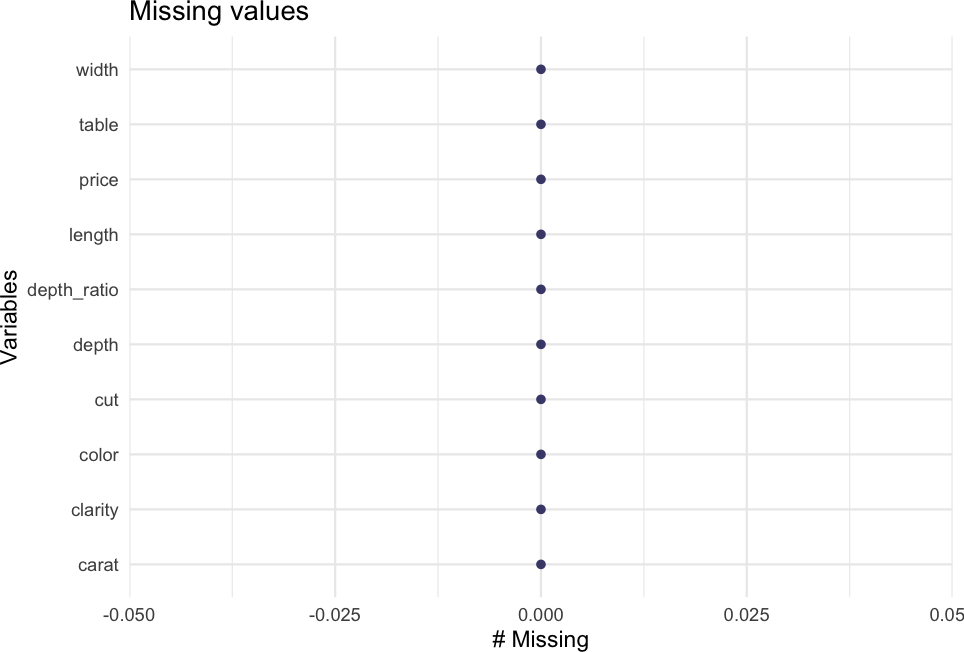
\includegraphics{Diamonds_files/figure-latex/Missing Values-1} \end{center}

\begin{Shaded}
\begin{Highlighting}[]
\DocumentationTok{\#\#\#\#\#\#\#\#\#\#\#\#\#\#\# carat no problems \#\#\#\#\#\#\#\#\#\#\#\#\#\#\#\#\#}

\DocumentationTok{\#\#\#\#\#\#\#\#\#\#\#\#\#\#\# cut \#\#\#\#\#\#\#\#\#\#\#\#\#\#\#\#\#\#\#\#\#\#\#\#\#\#\#\#\#\#\#}
\FunctionTok{unique}\NormalTok{(diamonds}\SpecialCharTok{$}\NormalTok{cut) }\CommentTok{\# Review unique values for cut}
\end{Highlighting}
\end{Shaded}

\begin{verbatim}
## [1] "Ideal"     "Premium"   "Good"      "Very Good" "Fair"
\end{verbatim}

\begin{Shaded}
\begin{Highlighting}[]
\CommentTok{\# Factor the cut to five level}
\NormalTok{diamonds}\SpecialCharTok{$}\NormalTok{cut }\OtherTok{\textless{}{-}} \FunctionTok{as.factor}\NormalTok{(diamonds}\SpecialCharTok{$}\NormalTok{cut) }

\CommentTok{\# Ordered from worst to best}
\NormalTok{diamonds}\SpecialCharTok{$}\NormalTok{cut }\OtherTok{\textless{}{-}} \FunctionTok{ordered}\NormalTok{(diamonds}\SpecialCharTok{$}\NormalTok{cut, }\AttributeTok{levels =} \FunctionTok{c}\NormalTok{(}\StringTok{"Fair"}\NormalTok{, }\StringTok{"Good"}\NormalTok{, }\StringTok{"Very Good"}\NormalTok{, }\StringTok{"Premium"}\NormalTok{, }\StringTok{"Ideal"}\NormalTok{)) }

\DocumentationTok{\#\#\#\#\#\#\#\#\#\#\#\#\#\#\# color \#\#\#\#\#\#\#\#\#\#\#\#\#\#\#\#\#\#\#\#\#\#\#\#\#\#\#\#}
\CommentTok{\# Review unique values for color}
\FunctionTok{unique}\NormalTok{(diamonds}\SpecialCharTok{$}\NormalTok{color) }
\end{Highlighting}
\end{Shaded}

\begin{verbatim}
## [1] "E" "I" "J" "H" "F" "G" "D"
\end{verbatim}

\begin{Shaded}
\begin{Highlighting}[]
\CommentTok{\# Factor the color to seven levels }
\NormalTok{diamonds}\SpecialCharTok{$}\NormalTok{color }\OtherTok{\textless{}{-}} \FunctionTok{as.factor}\NormalTok{(diamonds}\SpecialCharTok{$}\NormalTok{color) }

\CommentTok{\# Ordered from worst to best}
\NormalTok{diamonds}\SpecialCharTok{$}\NormalTok{color }\OtherTok{\textless{}{-}} \FunctionTok{ordered}\NormalTok{(diamonds}\SpecialCharTok{$}\NormalTok{color, }\AttributeTok{levels =} \FunctionTok{c}\NormalTok{(}\StringTok{"J"}\NormalTok{, }\StringTok{"I"}\NormalTok{, }\StringTok{"H"}\NormalTok{, }\StringTok{"G"}\NormalTok{, }\StringTok{"F"}\NormalTok{, }\StringTok{"E"}\NormalTok{, }\StringTok{"D"}\NormalTok{)) }

\DocumentationTok{\#\#\#\#\#\#\#\#\#\#\#\#\#\#\# clarity \#\#\#\#\#\#\#\#\#\#\#\#\#\#\#\#\#\#\#\#\#\#\#\#\#\#}
\CommentTok{\# Review unique values for clarity}
\FunctionTok{unique}\NormalTok{(diamonds}\SpecialCharTok{$}\NormalTok{clarity)}
\end{Highlighting}
\end{Shaded}

\begin{verbatim}
## [1] "SI2"  "SI1"  "VS1"  "VS2"  "VVS2" "VVS1" "I1"   "IF"
\end{verbatim}

\begin{Shaded}
\begin{Highlighting}[]
\CommentTok{\# Factor the clarity to eight levels }
\NormalTok{diamonds}\SpecialCharTok{$}\NormalTok{clarity }\OtherTok{\textless{}{-}} \FunctionTok{as.factor}\NormalTok{(diamonds}\SpecialCharTok{$}\NormalTok{clarity)}

\CommentTok{\# Ordered from worst to best}
\NormalTok{diamonds}\SpecialCharTok{$}\NormalTok{clarity }\OtherTok{\textless{}{-}} \FunctionTok{ordered}\NormalTok{(diamonds}\SpecialCharTok{$}\NormalTok{clarity, }\AttributeTok{levels =} \FunctionTok{c}\NormalTok{(}\StringTok{"I1"}\NormalTok{, }\StringTok{"SI2"}\NormalTok{, }\StringTok{"SI1"}\NormalTok{, }\StringTok{"VS2"}\NormalTok{, }\StringTok{"VS1"}\NormalTok{, }\StringTok{"VVS2"}\NormalTok{, }\StringTok{"VVS1"}\NormalTok{, }\StringTok{"IF"}\NormalTok{)) }

\DocumentationTok{\#\#\#\#\#\#\#\#\#\#\#\#\#\#\# table no problems\#\#\#\#\#\#\#\#\#\#\#\#\#\#\#\#\#}

\DocumentationTok{\#\#\#\#\#\#\#\#\#\#\#\#\#\#\# price no problems\#\#\#\#\#\#\#\#\#\#\#\#\#\#\#\#\#}

\DocumentationTok{\#\#\#\#\#\#\#\#\#\#\#\#\#\#\# Other Checks \#\#\#\#\#\#\#\#\#\#\#\#\#\#\#\#\#\#\#\#\#}

\CommentTok{\# Remove values of 0 for for dimensions which includes zeros in length and width}
\FunctionTok{nrow}\NormalTok{(diamonds[depth }\SpecialCharTok{\%in\%} \DecValTok{0}\NormalTok{,]) }\CommentTok{\# Remove 20 rows due to depth = 0.0}
\end{Highlighting}
\end{Shaded}

\begin{verbatim}
## [1] 20
\end{verbatim}

\begin{Shaded}
\begin{Highlighting}[]
\NormalTok{diamonds }\OtherTok{\textless{}{-}}\NormalTok{ diamonds[depth }\SpecialCharTok{\textgreater{}} \DecValTok{0}\NormalTok{, ] }\CommentTok{\# Include only values with depth greater than zero}

\CommentTok{\# Create formula to check the absolute value of length to width, comparison }
\NormalTok{diamonds[, subtraction }\SpecialCharTok{:}\ErrorTok{=} \FunctionTok{abs}\NormalTok{(length }\SpecialCharTok{{-}}\NormalTok{ width)]}
\FunctionTok{nrow}\NormalTok{(diamonds[subtraction}\SpecialCharTok{\textgreater{}}\DecValTok{10}\NormalTok{,]) }\CommentTok{\# Remove 2 rows due their extreme subtraction value (\textasciitilde{}59 and \textasciitilde{}26)}
\end{Highlighting}
\end{Shaded}

\begin{verbatim}
## [1] 2
\end{verbatim}

\begin{Shaded}
\begin{Highlighting}[]
\NormalTok{diamonds }\OtherTok{\textless{}{-}}\NormalTok{ diamonds[subtraction }\SpecialCharTok{\textless{}=} \DecValTok{10}\NormalTok{, ] }\CommentTok{\# Include only values with subtraction less than ten}

\CommentTok{\# Check if the Depth\_Ratio value corresponds to formula indicated in the description}
\NormalTok{diamonds[, depth\_check }\SpecialCharTok{:}\ErrorTok{=} \FunctionTok{round}\NormalTok{(}\DecValTok{100}\SpecialCharTok{*}\NormalTok{(}\DecValTok{2}\SpecialCharTok{*}\NormalTok{depth)}\SpecialCharTok{/}\NormalTok{((length }\SpecialCharTok{+}\NormalTok{ width)), }\DecValTok{1}\NormalTok{)]}
\NormalTok{diamonds[, diff }\SpecialCharTok{:}\ErrorTok{=} \FunctionTok{abs}\NormalTok{(depth\_check}\SpecialCharTok{{-}}\NormalTok{depth\_ratio)]}

\CommentTok{\# Create histogram to look at the differences between how much price is off between a calculated value and what the data provided}
\FunctionTok{hist}\NormalTok{(diamonds[diff }\SpecialCharTok{\textgreater{}=} \FloatTok{0.2} \SpecialCharTok{\&}\NormalTok{ diff }\SpecialCharTok{\textless{}} \DecValTok{1}\NormalTok{, diff], }\AttributeTok{breaks =}\DecValTok{50}\NormalTok{, }\AttributeTok{col =} \StringTok{"\#D8B365"}\NormalTok{, }\AttributeTok{border =} \StringTok{"\#D8B365"}\NormalTok{, }\AttributeTok{main =} \StringTok{"Threshold Differences"}\NormalTok{, }\AttributeTok{xlab =} \StringTok{"Predicted vs. Actual Difference"}\NormalTok{)}
\end{Highlighting}
\end{Shaded}

\begin{center}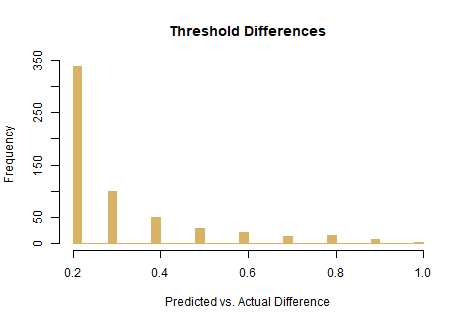
\includegraphics{Diamonds_files/figure-latex/Variables check-1} \end{center}

\begin{Shaded}
\begin{Highlighting}[]
\CommentTok{\# Threshold set to 0.3 due to ... (report)}
\FunctionTok{nrow}\NormalTok{(diamonds[diff }\SpecialCharTok{\textgreater{}} \FloatTok{0.3}\NormalTok{,]) }\CommentTok{\# We remove 268 rows}
\end{Highlighting}
\end{Shaded}

\begin{verbatim}
## [1] 253
\end{verbatim}

\begin{Shaded}
\begin{Highlighting}[]
\NormalTok{diamonds }\OtherTok{\textless{}{-}}\NormalTok{ diamonds[diff }\SpecialCharTok{\textless{}=} \FloatTok{0.3}\NormalTok{,]}


\CommentTok{\# Removed created columns needed to clean the data}
\NormalTok{diamonds[, subtraction }\SpecialCharTok{:}\ErrorTok{=} \ConstantTok{NULL}\NormalTok{]}
\NormalTok{diamonds[, depth\_check }\SpecialCharTok{:}\ErrorTok{=} \ConstantTok{NULL}\NormalTok{]}
\NormalTok{diamonds[, diff }\SpecialCharTok{:}\ErrorTok{=} \ConstantTok{NULL}\NormalTok{]}
\CommentTok{\# Total rows remove: 275 observations}
\end{Highlighting}
\end{Shaded}

\begin{Shaded}
\begin{Highlighting}[]
\CommentTok{\# Reorder data table to group like variable types }
\NormalTok{diamonds }\OtherTok{\textless{}{-}}\NormalTok{ diamonds[, }\FunctionTok{c}\NormalTok{(}\DecValTok{7}\NormalTok{, }\DecValTok{2}\SpecialCharTok{:}\DecValTok{4}\NormalTok{, }\DecValTok{1}\NormalTok{, }\DecValTok{8}\SpecialCharTok{:}\DecValTok{10}\NormalTok{, }\DecValTok{5}\SpecialCharTok{:}\DecValTok{6}\NormalTok{)]}
\end{Highlighting}
\end{Shaded}

\begin{Shaded}
\begin{Highlighting}[]
\CommentTok{\#Used ggpairs to create a scatterplot matrix between quantitative variables }
\FunctionTok{ggpairs}\NormalTok{(diamonds[, }\FunctionTok{c}\NormalTok{(}\DecValTok{1}\NormalTok{, }\DecValTok{5}\SpecialCharTok{:}\DecValTok{10}\NormalTok{)], }\AttributeTok{title =} \StringTok{"Scatterplot Matrix"}\NormalTok{,}
         \AttributeTok{proportions =} \StringTok{"auto"}\NormalTok{,}
         \AttributeTok{columnLabels =} \FunctionTok{c}\NormalTok{(}\StringTok{"Price"}\NormalTok{, }\StringTok{"Carat"}\NormalTok{, }\StringTok{"Length"}\NormalTok{, }\StringTok{"Width"}\NormalTok{, }\StringTok{"Depth"}\NormalTok{,}\StringTok{"Depth Ratio"}\NormalTok{,}\StringTok{"Table"}\NormalTok{),}
         \AttributeTok{upper =} \FunctionTok{list}\NormalTok{(}\AttributeTok{continuous =} \FunctionTok{wrap}\NormalTok{(}\StringTok{\textquotesingle{}cor\textquotesingle{}}\NormalTok{,}\AttributeTok{size =} \DecValTok{3}\NormalTok{)),) }\SpecialCharTok{+} \FunctionTok{theme\_light}\NormalTok{()}
\end{Highlighting}
\end{Shaded}

\begin{center}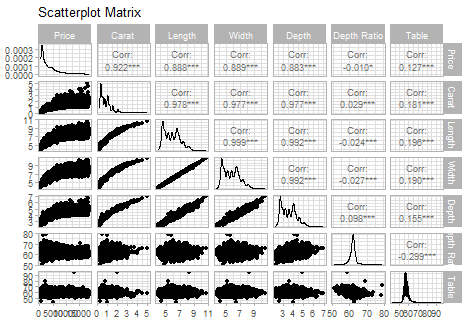
\includegraphics{Diamonds_files/figure-latex/ggpairs-1} \end{center}

\begin{Shaded}
\begin{Highlighting}[]
\CommentTok{\# Create plot that looks at carat and price}
\NormalTok{PCl1 }\OtherTok{\textless{}{-}} \FunctionTok{ggplot}\NormalTok{(}\FunctionTok{aes}\NormalTok{(}\AttributeTok{x =}\NormalTok{ carat, }\AttributeTok{y =}\NormalTok{ price), }\AttributeTok{data =}\NormalTok{ diamonds) }\SpecialCharTok{+} \FunctionTok{geom\_point}\NormalTok{(}\AttributeTok{alpha =} \FloatTok{0.5}\NormalTok{, }\AttributeTok{size =} \DecValTok{1}\NormalTok{, }\AttributeTok{position =} \StringTok{\textquotesingle{}jitter\textquotesingle{}}\NormalTok{,}\FunctionTok{aes}\NormalTok{(}\AttributeTok{color=}\NormalTok{clarity)) }\SpecialCharTok{+}
  \FunctionTok{scale\_color\_brewer}\NormalTok{(}\AttributeTok{type =} \StringTok{\textquotesingle{}div\textquotesingle{}}\NormalTok{, }\AttributeTok{guide =} \FunctionTok{guide\_legend}\NormalTok{(}\AttributeTok{title =} \StringTok{\textquotesingle{}Clarity\textquotesingle{}}\NormalTok{, }\AttributeTok{reverse =}\NormalTok{ T,}\AttributeTok{override.aes =} \FunctionTok{list}\NormalTok{(}\AttributeTok{alpha =} \DecValTok{1}\NormalTok{, }\AttributeTok{size =} \DecValTok{2}\NormalTok{)))       }\SpecialCharTok{+} \FunctionTok{ggtitle}\NormalTok{(}\StringTok{\textquotesingle{}Price by Carat and Clarity\textquotesingle{}}\NormalTok{) }\SpecialCharTok{+} \FunctionTok{theme\_classic}\NormalTok{()}

\CommentTok{\# Create plot that looks at length and price}
\NormalTok{PCl2 }\OtherTok{\textless{}{-}} \FunctionTok{ggplot}\NormalTok{(}\FunctionTok{aes}\NormalTok{(}\AttributeTok{x =}\NormalTok{ length, }\AttributeTok{y =}\NormalTok{ price), }\AttributeTok{data =}\NormalTok{ diamonds) }\SpecialCharTok{+} \FunctionTok{geom\_point}\NormalTok{(}\AttributeTok{alpha =} \FloatTok{0.5}\NormalTok{, }\AttributeTok{size =} \DecValTok{1}\NormalTok{, }\AttributeTok{position =} \StringTok{\textquotesingle{}jitter\textquotesingle{}}\NormalTok{,}\FunctionTok{aes}\NormalTok{(}\AttributeTok{color=}\NormalTok{clarity)) }\SpecialCharTok{+}
  \FunctionTok{scale\_color\_brewer}\NormalTok{(}\AttributeTok{type =} \StringTok{\textquotesingle{}div\textquotesingle{}}\NormalTok{, }\AttributeTok{guide =} \FunctionTok{guide\_legend}\NormalTok{(}\AttributeTok{title =} \StringTok{\textquotesingle{}Clarity\textquotesingle{}}\NormalTok{, }\AttributeTok{reverse =}\NormalTok{ T,}\AttributeTok{override.aes =} \FunctionTok{list}\NormalTok{(}\AttributeTok{alpha =} \DecValTok{1}\NormalTok{, }\AttributeTok{size =} \DecValTok{2}\NormalTok{)))       }\SpecialCharTok{+} \FunctionTok{ggtitle}\NormalTok{(}\StringTok{\textquotesingle{}Price by Length and Clarity\textquotesingle{}}\NormalTok{) }\SpecialCharTok{+} \FunctionTok{theme\_classic}\NormalTok{()}

\CommentTok{\# Create plot that looks at width and price}
\NormalTok{PCl3 }\OtherTok{\textless{}{-}} \FunctionTok{ggplot}\NormalTok{(}\FunctionTok{aes}\NormalTok{(}\AttributeTok{x =}\NormalTok{ width, }\AttributeTok{y =}\NormalTok{ price), }\AttributeTok{data =}\NormalTok{ diamonds) }\SpecialCharTok{+} \FunctionTok{geom\_point}\NormalTok{(}\AttributeTok{alpha =} \FloatTok{0.5}\NormalTok{, }\AttributeTok{size =} \DecValTok{1}\NormalTok{, }\AttributeTok{position =} \StringTok{\textquotesingle{}jitter\textquotesingle{}}\NormalTok{,}\FunctionTok{aes}\NormalTok{(}\AttributeTok{color=}\NormalTok{clarity)) }\SpecialCharTok{+}
  \FunctionTok{scale\_color\_brewer}\NormalTok{(}\AttributeTok{type =} \StringTok{\textquotesingle{}div\textquotesingle{}}\NormalTok{, }\AttributeTok{guide =} \FunctionTok{guide\_legend}\NormalTok{(}\AttributeTok{title =} \StringTok{\textquotesingle{}Clarity\textquotesingle{}}\NormalTok{, }\AttributeTok{reverse =}\NormalTok{ T,}\AttributeTok{override.aes =} \FunctionTok{list}\NormalTok{(}\AttributeTok{alpha =} \DecValTok{1}\NormalTok{, }\AttributeTok{size =} \DecValTok{2}\NormalTok{)))       }\SpecialCharTok{+} \FunctionTok{ggtitle}\NormalTok{(}\StringTok{\textquotesingle{}Price by Width and Clarity\textquotesingle{}}\NormalTok{) }\SpecialCharTok{+} \FunctionTok{theme\_classic}\NormalTok{()}

\CommentTok{\# Create plot that looks at depth and price}
\NormalTok{PCl4 }\OtherTok{\textless{}{-}} \FunctionTok{ggplot}\NormalTok{(}\FunctionTok{aes}\NormalTok{(}\AttributeTok{x =}\NormalTok{ depth, }\AttributeTok{y =}\NormalTok{ price), }\AttributeTok{data =}\NormalTok{ diamonds) }\SpecialCharTok{+} \FunctionTok{geom\_point}\NormalTok{(}\AttributeTok{alpha =} \FloatTok{0.5}\NormalTok{, }\AttributeTok{size =} \DecValTok{1}\NormalTok{, }\AttributeTok{position =} \StringTok{\textquotesingle{}jitter\textquotesingle{}}\NormalTok{,}\FunctionTok{aes}\NormalTok{(}\AttributeTok{color=}\NormalTok{clarity)) }\SpecialCharTok{+}
  \FunctionTok{scale\_color\_brewer}\NormalTok{(}\AttributeTok{type =} \StringTok{\textquotesingle{}div\textquotesingle{}}\NormalTok{, }\AttributeTok{guide =} \FunctionTok{guide\_legend}\NormalTok{(}\AttributeTok{title =} \StringTok{\textquotesingle{}Clarity\textquotesingle{}}\NormalTok{, }\AttributeTok{reverse =}\NormalTok{ T,}\AttributeTok{override.aes =} \FunctionTok{list}\NormalTok{(}\AttributeTok{alpha =} \DecValTok{1}\NormalTok{, }\AttributeTok{size =} \DecValTok{2}\NormalTok{)))       }\SpecialCharTok{+} \FunctionTok{ggtitle}\NormalTok{(}\StringTok{\textquotesingle{}Price by Depth and Clarity\textquotesingle{}}\NormalTok{) }\SpecialCharTok{+} \FunctionTok{theme\_classic}\NormalTok{()}

\CommentTok{\# Create plot that looks at depth\_ratio and price}
\NormalTok{PCl5 }\OtherTok{\textless{}{-}} \FunctionTok{ggplot}\NormalTok{(}\FunctionTok{aes}\NormalTok{(}\AttributeTok{x =}\NormalTok{ depth\_ratio, }\AttributeTok{y =}\NormalTok{ price), }\AttributeTok{data =}\NormalTok{ diamonds) }\SpecialCharTok{+} \FunctionTok{geom\_point}\NormalTok{(}\AttributeTok{alpha =} \FloatTok{0.5}\NormalTok{, }\AttributeTok{size =} \DecValTok{1}\NormalTok{, }\AttributeTok{position =} \StringTok{\textquotesingle{}jitter\textquotesingle{}}\NormalTok{,}\FunctionTok{aes}\NormalTok{(}\AttributeTok{color=}\NormalTok{clarity))  }\SpecialCharTok{+} \FunctionTok{scale\_color\_brewer}\NormalTok{(}\AttributeTok{type =} \StringTok{\textquotesingle{}div\textquotesingle{}}\NormalTok{, }\AttributeTok{guide =} \FunctionTok{guide\_legend}\NormalTok{(}\AttributeTok{title =} \StringTok{\textquotesingle{}Clarity\textquotesingle{}}\NormalTok{, }\AttributeTok{reverse =}\NormalTok{ T,}\AttributeTok{override.aes =} \FunctionTok{list}\NormalTok{(}\AttributeTok{alpha =} \DecValTok{1}\NormalTok{, }\AttributeTok{size =} \DecValTok{2}\NormalTok{))) }\SpecialCharTok{+} \FunctionTok{ggtitle}\NormalTok{(}\StringTok{\textquotesingle{}Price by Depth Ratio and Clarity\textquotesingle{}}\NormalTok{)  }\SpecialCharTok{+} \FunctionTok{theme\_classic}\NormalTok{() }\SpecialCharTok{+} \FunctionTok{geom\_vline}\NormalTok{(}\AttributeTok{xintercept=}\FunctionTok{mean}\NormalTok{(diamonds}\SpecialCharTok{$}\NormalTok{depth\_ratio), }\AttributeTok{size =} \DecValTok{1}\NormalTok{, }\AttributeTok{color =} \StringTok{"black"}\NormalTok{) }\SpecialCharTok{+} \FunctionTok{geom\_vline}\NormalTok{(}\AttributeTok{xintercept=}\DecValTok{59}\NormalTok{, }\AttributeTok{size =} \DecValTok{1}\NormalTok{, }\AttributeTok{color =} \StringTok{"red"}\NormalTok{) }\SpecialCharTok{+} \FunctionTok{geom\_vline}\NormalTok{(}\AttributeTok{xintercept=}\FloatTok{62.3}\NormalTok{, }\AttributeTok{size =} \DecValTok{1}\NormalTok{, }\AttributeTok{color =} \StringTok{"red"}\NormalTok{)}

\CommentTok{\# Create plot that looks at table and price}
\NormalTok{PCl6 }\OtherTok{\textless{}{-}} \FunctionTok{ggplot}\NormalTok{(}\FunctionTok{aes}\NormalTok{(}\AttributeTok{x =}\NormalTok{ table, }\AttributeTok{y =}\NormalTok{ price), }\AttributeTok{data =}\NormalTok{ diamonds) }\SpecialCharTok{+}  \FunctionTok{geom\_point}\NormalTok{(}\AttributeTok{alpha =} \FloatTok{0.5}\NormalTok{, }\AttributeTok{size =} \DecValTok{1}\NormalTok{, }\AttributeTok{position =} \StringTok{\textquotesingle{}jitter\textquotesingle{}}\NormalTok{,}\FunctionTok{aes}\NormalTok{(}\AttributeTok{color=}\NormalTok{clarity))  }\SpecialCharTok{+} \FunctionTok{scale\_color\_brewer}\NormalTok{(}\AttributeTok{type =} \StringTok{\textquotesingle{}div\textquotesingle{}}\NormalTok{, }\AttributeTok{guide =} \FunctionTok{guide\_legend}\NormalTok{(}\AttributeTok{title =} \StringTok{\textquotesingle{}Clarity\textquotesingle{}}\NormalTok{, }\AttributeTok{reverse =}\NormalTok{ T,}\AttributeTok{override.aes =} \FunctionTok{list}\NormalTok{(}\AttributeTok{alpha =} \DecValTok{1}\NormalTok{, }\AttributeTok{size =} \DecValTok{2}\NormalTok{))) }\SpecialCharTok{+} \FunctionTok{ggtitle}\NormalTok{(}\StringTok{\textquotesingle{}Price by Table and Clarity\textquotesingle{}}\NormalTok{)}\SpecialCharTok{+} \FunctionTok{theme\_classic}\NormalTok{() }\SpecialCharTok{+} \FunctionTok{geom\_vline}\NormalTok{(}\AttributeTok{xintercept=}\FunctionTok{mean}\NormalTok{(diamonds}\SpecialCharTok{$}\NormalTok{table), }\AttributeTok{size =} \DecValTok{1}\NormalTok{, }\AttributeTok{color =} \StringTok{"black"}\NormalTok{)}

\CommentTok{\# Arrange ggplots into one frame}
\FunctionTok{ggarrange}\NormalTok{(PCl1, PCl2, PCl3,PCl4, PCl5, PCl6,}
                    \AttributeTok{ncol =} \DecValTok{2}\NormalTok{, }\AttributeTok{nrow =} \DecValTok{3}\NormalTok{)}
\end{Highlighting}
\end{Shaded}

\begin{center}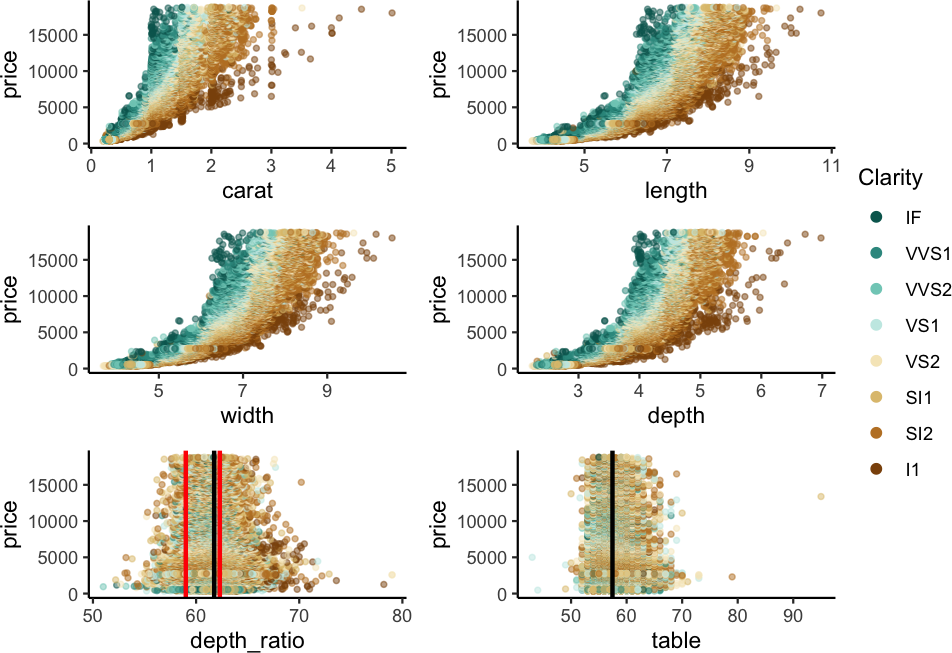
\includegraphics{Diamonds_files/figure-latex/Price by X and Clarity-1} \end{center}

\begin{Shaded}
\begin{Highlighting}[]
\CommentTok{\# Create plot that looks at carat and price}
\NormalTok{PCo1 }\OtherTok{\textless{}{-}} \FunctionTok{ggplot}\NormalTok{(}\FunctionTok{aes}\NormalTok{(}\AttributeTok{x =}\NormalTok{ carat, }\AttributeTok{y =}\NormalTok{ price), }\AttributeTok{data =}\NormalTok{ diamonds) }\SpecialCharTok{+} \FunctionTok{geom\_point}\NormalTok{(}\AttributeTok{alpha =} \FloatTok{0.5}\NormalTok{, }\AttributeTok{size =} \DecValTok{1}\NormalTok{, }\AttributeTok{position =} \StringTok{\textquotesingle{}jitter\textquotesingle{}}\NormalTok{,}\FunctionTok{aes}\NormalTok{(}\AttributeTok{color=}\NormalTok{color)) }\SpecialCharTok{+}
  \FunctionTok{scale\_color\_brewer}\NormalTok{(}\AttributeTok{type =} \StringTok{\textquotesingle{}div\textquotesingle{}}\NormalTok{, }\AttributeTok{guide =} \FunctionTok{guide\_legend}\NormalTok{(}\AttributeTok{title =} \StringTok{\textquotesingle{}Color\textquotesingle{}}\NormalTok{, }\AttributeTok{reverse =}\NormalTok{ T,}\AttributeTok{override.aes =} \FunctionTok{list}\NormalTok{(}\AttributeTok{alpha =} \DecValTok{1}\NormalTok{, }\AttributeTok{size =} \DecValTok{2}\NormalTok{)))       }\SpecialCharTok{+} \FunctionTok{ggtitle}\NormalTok{(}\StringTok{\textquotesingle{}Price by Carat and Color\textquotesingle{}}\NormalTok{) }\SpecialCharTok{+} \FunctionTok{theme\_classic}\NormalTok{()}

\CommentTok{\# Create plot that looks at length and price}
\NormalTok{PCo2 }\OtherTok{\textless{}{-}} \FunctionTok{ggplot}\NormalTok{(}\FunctionTok{aes}\NormalTok{(}\AttributeTok{x =}\NormalTok{ length, }\AttributeTok{y =}\NormalTok{ price), }\AttributeTok{data =}\NormalTok{ diamonds) }\SpecialCharTok{+} \FunctionTok{geom\_point}\NormalTok{(}\AttributeTok{alpha =} \FloatTok{0.5}\NormalTok{, }\AttributeTok{size =} \DecValTok{1}\NormalTok{, }\AttributeTok{position =} \StringTok{\textquotesingle{}jitter\textquotesingle{}}\NormalTok{,}\FunctionTok{aes}\NormalTok{(}\AttributeTok{color=}\NormalTok{color)) }\SpecialCharTok{+}
  \FunctionTok{scale\_color\_brewer}\NormalTok{(}\AttributeTok{type =} \StringTok{\textquotesingle{}div\textquotesingle{}}\NormalTok{, }\AttributeTok{guide =} \FunctionTok{guide\_legend}\NormalTok{(}\AttributeTok{title =} \StringTok{\textquotesingle{}Color\textquotesingle{}}\NormalTok{, }\AttributeTok{reverse =}\NormalTok{ T,}\AttributeTok{override.aes =} \FunctionTok{list}\NormalTok{(}\AttributeTok{alpha =} \DecValTok{1}\NormalTok{, }\AttributeTok{size =} \DecValTok{2}\NormalTok{)))       }\SpecialCharTok{+} \FunctionTok{ggtitle}\NormalTok{(}\StringTok{\textquotesingle{}Price by Length and Color\textquotesingle{}}\NormalTok{) }\SpecialCharTok{+} \FunctionTok{theme\_classic}\NormalTok{()}

\CommentTok{\# Create plot that looks at width and price}
\NormalTok{PCo3 }\OtherTok{\textless{}{-}} \FunctionTok{ggplot}\NormalTok{(}\FunctionTok{aes}\NormalTok{(}\AttributeTok{x =}\NormalTok{ width, }\AttributeTok{y =}\NormalTok{ price), }\AttributeTok{data =}\NormalTok{ diamonds) }\SpecialCharTok{+} \FunctionTok{geom\_point}\NormalTok{(}\AttributeTok{alpha =} \FloatTok{0.5}\NormalTok{, }\AttributeTok{size =} \DecValTok{1}\NormalTok{, }\AttributeTok{position =} \StringTok{\textquotesingle{}jitter\textquotesingle{}}\NormalTok{,}\FunctionTok{aes}\NormalTok{(}\AttributeTok{color=}\NormalTok{color)) }\SpecialCharTok{+}
  \FunctionTok{scale\_color\_brewer}\NormalTok{(}\AttributeTok{type =} \StringTok{\textquotesingle{}div\textquotesingle{}}\NormalTok{, }\AttributeTok{guide =} \FunctionTok{guide\_legend}\NormalTok{(}\AttributeTok{title =} \StringTok{\textquotesingle{}Color\textquotesingle{}}\NormalTok{, }\AttributeTok{reverse =}\NormalTok{ T,}\AttributeTok{override.aes =} \FunctionTok{list}\NormalTok{(}\AttributeTok{alpha =} \DecValTok{1}\NormalTok{, }\AttributeTok{size =} \DecValTok{2}\NormalTok{)))       }\SpecialCharTok{+} \FunctionTok{ggtitle}\NormalTok{(}\StringTok{\textquotesingle{}Price by Width and Color\textquotesingle{}}\NormalTok{) }\SpecialCharTok{+} \FunctionTok{theme\_classic}\NormalTok{()}

\CommentTok{\# Create plot that looks at depth and price}
\NormalTok{PCo4 }\OtherTok{\textless{}{-}} \FunctionTok{ggplot}\NormalTok{(}\FunctionTok{aes}\NormalTok{(}\AttributeTok{x =}\NormalTok{ depth, }\AttributeTok{y =}\NormalTok{ price), }\AttributeTok{data =}\NormalTok{ diamonds) }\SpecialCharTok{+} \FunctionTok{geom\_point}\NormalTok{(}\AttributeTok{alpha =} \FloatTok{0.5}\NormalTok{, }\AttributeTok{size =} \DecValTok{1}\NormalTok{, }\AttributeTok{position =} \StringTok{\textquotesingle{}jitter\textquotesingle{}}\NormalTok{,}\FunctionTok{aes}\NormalTok{(}\AttributeTok{color=}\NormalTok{color)) }\SpecialCharTok{+}
  \FunctionTok{scale\_color\_brewer}\NormalTok{(}\AttributeTok{type =} \StringTok{\textquotesingle{}div\textquotesingle{}}\NormalTok{, }\AttributeTok{guide =} \FunctionTok{guide\_legend}\NormalTok{(}\AttributeTok{title =} \StringTok{\textquotesingle{}Color\textquotesingle{}}\NormalTok{, }\AttributeTok{reverse =}\NormalTok{ T,}\AttributeTok{override.aes =} \FunctionTok{list}\NormalTok{(}\AttributeTok{alpha =} \DecValTok{1}\NormalTok{, }\AttributeTok{size =} \DecValTok{2}\NormalTok{)))       }\SpecialCharTok{+} \FunctionTok{ggtitle}\NormalTok{(}\StringTok{\textquotesingle{}Price by Depth and Color\textquotesingle{}}\NormalTok{) }\SpecialCharTok{+} \FunctionTok{theme\_classic}\NormalTok{()}

\CommentTok{\# Create plot that looks at depth\_ratio and price}
\NormalTok{PCo5 }\OtherTok{\textless{}{-}} \FunctionTok{ggplot}\NormalTok{(}\FunctionTok{aes}\NormalTok{(}\AttributeTok{x =}\NormalTok{ depth\_ratio, }\AttributeTok{y =}\NormalTok{ price), }\AttributeTok{data =}\NormalTok{ diamonds) }\SpecialCharTok{+} \FunctionTok{geom\_point}\NormalTok{(}\AttributeTok{alpha =} \FloatTok{0.5}\NormalTok{, }\AttributeTok{size =} \DecValTok{1}\NormalTok{, }\AttributeTok{position =} \StringTok{\textquotesingle{}jitter\textquotesingle{}}\NormalTok{,}\FunctionTok{aes}\NormalTok{(}\AttributeTok{color=}\NormalTok{color))  }\SpecialCharTok{+} \FunctionTok{scale\_color\_brewer}\NormalTok{(}\AttributeTok{type =} \StringTok{\textquotesingle{}div\textquotesingle{}}\NormalTok{, }\AttributeTok{guide =} \FunctionTok{guide\_legend}\NormalTok{(}\AttributeTok{title =} \StringTok{\textquotesingle{}Color\textquotesingle{}}\NormalTok{, }\AttributeTok{reverse =}\NormalTok{ T,}\AttributeTok{override.aes =} \FunctionTok{list}\NormalTok{(}\AttributeTok{alpha =} \DecValTok{1}\NormalTok{, }\AttributeTok{size =} \DecValTok{2}\NormalTok{))) }\SpecialCharTok{+} \FunctionTok{ggtitle}\NormalTok{(}\StringTok{\textquotesingle{}Price by Depth Ratio and Color\textquotesingle{}}\NormalTok{)  }\SpecialCharTok{+} \FunctionTok{theme\_classic}\NormalTok{() }\SpecialCharTok{+} \FunctionTok{geom\_vline}\NormalTok{(}\AttributeTok{xintercept=}\FunctionTok{mean}\NormalTok{(diamonds}\SpecialCharTok{$}\NormalTok{depth\_ratio), }\AttributeTok{size =} \DecValTok{1}\NormalTok{, }\AttributeTok{color =} \StringTok{"black"}\NormalTok{)  }\SpecialCharTok{+} \FunctionTok{geom\_vline}\NormalTok{(}\AttributeTok{xintercept=}\DecValTok{59}\NormalTok{, }\AttributeTok{size =} \DecValTok{1}\NormalTok{, }\AttributeTok{color =} \StringTok{"red"}\NormalTok{) }\SpecialCharTok{+} \FunctionTok{geom\_vline}\NormalTok{(}\AttributeTok{xintercept=}\FloatTok{62.3}\NormalTok{, }\AttributeTok{size =} \DecValTok{1}\NormalTok{, }\AttributeTok{color =} \StringTok{"red"}\NormalTok{)}

\CommentTok{\# Create plot that looks at table and price}
\NormalTok{PCo6 }\OtherTok{\textless{}{-}} \FunctionTok{ggplot}\NormalTok{(}\FunctionTok{aes}\NormalTok{(}\AttributeTok{x =}\NormalTok{ table, }\AttributeTok{y =}\NormalTok{ price), }\AttributeTok{data =}\NormalTok{ diamonds) }\SpecialCharTok{+}  \FunctionTok{geom\_point}\NormalTok{(}\AttributeTok{alpha =} \FloatTok{0.5}\NormalTok{, }\AttributeTok{size =} \DecValTok{1}\NormalTok{, }\AttributeTok{position =} \StringTok{\textquotesingle{}jitter\textquotesingle{}}\NormalTok{,}\FunctionTok{aes}\NormalTok{(}\AttributeTok{color=}\NormalTok{color))  }\SpecialCharTok{+} \FunctionTok{scale\_color\_brewer}\NormalTok{(}\AttributeTok{type =} \StringTok{\textquotesingle{}div\textquotesingle{}}\NormalTok{, }\AttributeTok{guide =} \FunctionTok{guide\_legend}\NormalTok{(}\AttributeTok{title =} \StringTok{\textquotesingle{}Color\textquotesingle{}}\NormalTok{, }\AttributeTok{reverse =}\NormalTok{ T,}\AttributeTok{override.aes =} \FunctionTok{list}\NormalTok{(}\AttributeTok{alpha =} \DecValTok{1}\NormalTok{, }\AttributeTok{size =} \DecValTok{2}\NormalTok{))) }\SpecialCharTok{+} \FunctionTok{ggtitle}\NormalTok{(}\StringTok{\textquotesingle{}Price by Table and Color\textquotesingle{}}\NormalTok{)}\SpecialCharTok{+} \FunctionTok{theme\_classic}\NormalTok{() }\SpecialCharTok{+} \FunctionTok{geom\_vline}\NormalTok{(}\AttributeTok{xintercept=}\FunctionTok{mean}\NormalTok{(diamonds}\SpecialCharTok{$}\NormalTok{table), }\AttributeTok{size =} \DecValTok{1}\NormalTok{, }\AttributeTok{color =} \StringTok{"black"}\NormalTok{)}

\CommentTok{\# Arrange ggplots into one frame}
\FunctionTok{ggarrange}\NormalTok{(PCo1, PCo2, PCo3,PCo4, PCo5, PCo6,}
                    \AttributeTok{ncol =} \DecValTok{2}\NormalTok{, }\AttributeTok{nrow =} \DecValTok{3}\NormalTok{)}
\end{Highlighting}
\end{Shaded}

\begin{center}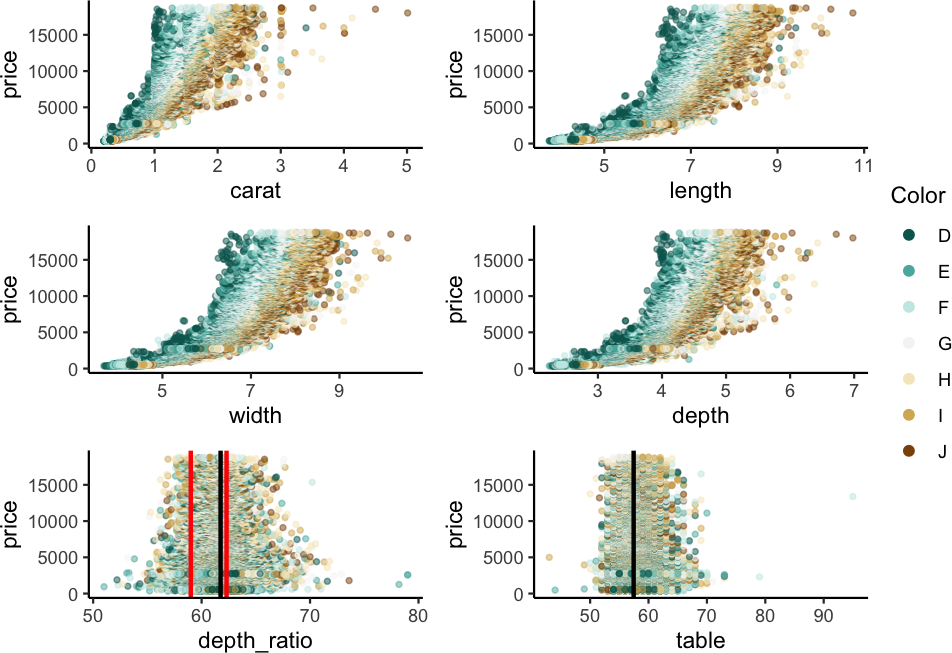
\includegraphics{Diamonds_files/figure-latex/Price by X and Color-1} \end{center}

\begin{Shaded}
\begin{Highlighting}[]
\CommentTok{\# Create plot that looks at carat and price}
\NormalTok{PCu1 }\OtherTok{\textless{}{-}} \FunctionTok{ggplot}\NormalTok{(}\FunctionTok{aes}\NormalTok{(}\AttributeTok{x =}\NormalTok{ carat, }\AttributeTok{y =}\NormalTok{ price), }\AttributeTok{data =}\NormalTok{ diamonds) }\SpecialCharTok{+} \FunctionTok{geom\_point}\NormalTok{(}\AttributeTok{alpha =} \FloatTok{0.5}\NormalTok{, }\AttributeTok{size =} \DecValTok{1}\NormalTok{, }\AttributeTok{position =} \StringTok{\textquotesingle{}jitter\textquotesingle{}}\NormalTok{,}\FunctionTok{aes}\NormalTok{(}\AttributeTok{color=}\NormalTok{cut)) }\SpecialCharTok{+}
  \FunctionTok{scale\_color\_brewer}\NormalTok{(}\AttributeTok{type =} \StringTok{\textquotesingle{}div\textquotesingle{}}\NormalTok{, }\AttributeTok{guide =} \FunctionTok{guide\_legend}\NormalTok{(}\AttributeTok{title =} \StringTok{\textquotesingle{}Cut\textquotesingle{}}\NormalTok{, }\AttributeTok{reverse =}\NormalTok{ T,}\AttributeTok{override.aes =} \FunctionTok{list}\NormalTok{(}\AttributeTok{alpha =} \DecValTok{1}\NormalTok{, }\AttributeTok{size =} \DecValTok{2}\NormalTok{)))       }\SpecialCharTok{+} \FunctionTok{ggtitle}\NormalTok{(}\StringTok{\textquotesingle{}Price by Carat and Cut\textquotesingle{}}\NormalTok{) }\SpecialCharTok{+} \FunctionTok{theme\_classic}\NormalTok{()}

\CommentTok{\# Create plot that looks at length and price}
\NormalTok{PCu2 }\OtherTok{\textless{}{-}} \FunctionTok{ggplot}\NormalTok{(}\FunctionTok{aes}\NormalTok{(}\AttributeTok{x =}\NormalTok{ length, }\AttributeTok{y =}\NormalTok{ price), }\AttributeTok{data =}\NormalTok{ diamonds) }\SpecialCharTok{+} \FunctionTok{geom\_point}\NormalTok{(}\AttributeTok{alpha =} \FloatTok{0.5}\NormalTok{, }\AttributeTok{size =} \DecValTok{1}\NormalTok{, }\AttributeTok{position =} \StringTok{\textquotesingle{}jitter\textquotesingle{}}\NormalTok{,}\FunctionTok{aes}\NormalTok{(}\AttributeTok{color=}\NormalTok{cut)) }\SpecialCharTok{+}
  \FunctionTok{scale\_color\_brewer}\NormalTok{(}\AttributeTok{type =} \StringTok{\textquotesingle{}div\textquotesingle{}}\NormalTok{, }\AttributeTok{guide =} \FunctionTok{guide\_legend}\NormalTok{(}\AttributeTok{title =} \StringTok{\textquotesingle{}Cut\textquotesingle{}}\NormalTok{, }\AttributeTok{reverse =}\NormalTok{ T,}\AttributeTok{override.aes =} \FunctionTok{list}\NormalTok{(}\AttributeTok{alpha =} \DecValTok{1}\NormalTok{, }\AttributeTok{size =} \DecValTok{2}\NormalTok{)))       }\SpecialCharTok{+} \FunctionTok{ggtitle}\NormalTok{(}\StringTok{\textquotesingle{}Price by Length and Cut\textquotesingle{}}\NormalTok{) }\SpecialCharTok{+} \FunctionTok{theme\_classic}\NormalTok{()}

\CommentTok{\# Create plot that looks at width and price}
\NormalTok{PCu3 }\OtherTok{\textless{}{-}} \FunctionTok{ggplot}\NormalTok{(}\FunctionTok{aes}\NormalTok{(}\AttributeTok{x =}\NormalTok{ width, }\AttributeTok{y =}\NormalTok{ price), }\AttributeTok{data =}\NormalTok{ diamonds) }\SpecialCharTok{+} \FunctionTok{geom\_point}\NormalTok{(}\AttributeTok{alpha =} \FloatTok{0.5}\NormalTok{, }\AttributeTok{size =} \DecValTok{1}\NormalTok{, }\AttributeTok{position =} \StringTok{\textquotesingle{}jitter\textquotesingle{}}\NormalTok{,}\FunctionTok{aes}\NormalTok{(}\AttributeTok{color=}\NormalTok{cut)) }\SpecialCharTok{+}
  \FunctionTok{scale\_color\_brewer}\NormalTok{(}\AttributeTok{type =} \StringTok{\textquotesingle{}div\textquotesingle{}}\NormalTok{, }\AttributeTok{guide =} \FunctionTok{guide\_legend}\NormalTok{(}\AttributeTok{title =} \StringTok{\textquotesingle{}Cut\textquotesingle{}}\NormalTok{, }\AttributeTok{reverse =}\NormalTok{ T,}\AttributeTok{override.aes =} \FunctionTok{list}\NormalTok{(}\AttributeTok{alpha =} \DecValTok{1}\NormalTok{, }\AttributeTok{size =} \DecValTok{2}\NormalTok{)))       }\SpecialCharTok{+} \FunctionTok{ggtitle}\NormalTok{(}\StringTok{\textquotesingle{}Price by Width and Cut\textquotesingle{}}\NormalTok{) }\SpecialCharTok{+} \FunctionTok{theme\_classic}\NormalTok{()}

\CommentTok{\# Create plot that looks at depth and price}
\NormalTok{PCu4 }\OtherTok{\textless{}{-}} \FunctionTok{ggplot}\NormalTok{(}\FunctionTok{aes}\NormalTok{(}\AttributeTok{x =}\NormalTok{ depth, }\AttributeTok{y =}\NormalTok{ price), }\AttributeTok{data =}\NormalTok{ diamonds) }\SpecialCharTok{+} \FunctionTok{geom\_point}\NormalTok{(}\AttributeTok{alpha =} \FloatTok{0.5}\NormalTok{, }\AttributeTok{size =} \DecValTok{1}\NormalTok{, }\AttributeTok{position =} \StringTok{\textquotesingle{}jitter\textquotesingle{}}\NormalTok{,}\FunctionTok{aes}\NormalTok{(}\AttributeTok{color=}\NormalTok{cut)) }\SpecialCharTok{+}
  \FunctionTok{scale\_color\_brewer}\NormalTok{(}\AttributeTok{type =} \StringTok{\textquotesingle{}div\textquotesingle{}}\NormalTok{, }\AttributeTok{guide =} \FunctionTok{guide\_legend}\NormalTok{(}\AttributeTok{title =} \StringTok{\textquotesingle{}Cut\textquotesingle{}}\NormalTok{, }\AttributeTok{reverse =}\NormalTok{ T,}\AttributeTok{override.aes =} \FunctionTok{list}\NormalTok{(}\AttributeTok{alpha =} \DecValTok{1}\NormalTok{, }\AttributeTok{size =} \DecValTok{2}\NormalTok{)))       }\SpecialCharTok{+} \FunctionTok{ggtitle}\NormalTok{(}\StringTok{\textquotesingle{}Price by Depth and Cut\textquotesingle{}}\NormalTok{) }\SpecialCharTok{+} \FunctionTok{theme\_classic}\NormalTok{()}

\CommentTok{\# Create plot that looks at depth\_ratio and price}
\NormalTok{PCu5 }\OtherTok{\textless{}{-}} \FunctionTok{ggplot}\NormalTok{(}\FunctionTok{aes}\NormalTok{(}\AttributeTok{x =}\NormalTok{ depth\_ratio, }\AttributeTok{y =}\NormalTok{ price), }\AttributeTok{data =}\NormalTok{ diamonds) }\SpecialCharTok{+} \FunctionTok{geom\_point}\NormalTok{(}\AttributeTok{alpha =} \FloatTok{0.5}\NormalTok{, }\AttributeTok{size =} \DecValTok{1}\NormalTok{, }\AttributeTok{position =} \StringTok{\textquotesingle{}jitter\textquotesingle{}}\NormalTok{,}\FunctionTok{aes}\NormalTok{(}\AttributeTok{color=}\NormalTok{cut))  }\SpecialCharTok{+} \FunctionTok{scale\_color\_brewer}\NormalTok{(}\AttributeTok{type =} \StringTok{\textquotesingle{}div\textquotesingle{}}\NormalTok{, }\AttributeTok{guide =} \FunctionTok{guide\_legend}\NormalTok{(}\AttributeTok{title =} \StringTok{\textquotesingle{}Cut\textquotesingle{}}\NormalTok{, }\AttributeTok{reverse =}\NormalTok{ T,}\AttributeTok{override.aes =} \FunctionTok{list}\NormalTok{(}\AttributeTok{alpha =} \DecValTok{1}\NormalTok{, }\AttributeTok{size =} \DecValTok{2}\NormalTok{))) }\SpecialCharTok{+} \FunctionTok{ggtitle}\NormalTok{(}\StringTok{\textquotesingle{}Price by Depth Ratio and Cut\textquotesingle{}}\NormalTok{)  }\SpecialCharTok{+} \FunctionTok{theme\_classic}\NormalTok{() }\SpecialCharTok{+} \FunctionTok{geom\_vline}\NormalTok{(}\AttributeTok{xintercept=}\FunctionTok{mean}\NormalTok{(diamonds}\SpecialCharTok{$}\NormalTok{depth\_ratio), }\AttributeTok{size =} \DecValTok{1}\NormalTok{, }\AttributeTok{color =} \StringTok{"black"}\NormalTok{) }\SpecialCharTok{+} \FunctionTok{geom\_vline}\NormalTok{(}\AttributeTok{xintercept=}\DecValTok{59}\NormalTok{, }\AttributeTok{size =} \DecValTok{1}\NormalTok{, }\AttributeTok{color =} \StringTok{"red"}\NormalTok{) }\SpecialCharTok{+} \FunctionTok{geom\_vline}\NormalTok{(}\AttributeTok{xintercept=}\FloatTok{62.3}\NormalTok{, }\AttributeTok{size =} \DecValTok{1}\NormalTok{, }\AttributeTok{color =} \StringTok{"red"}\NormalTok{)}

\CommentTok{\# Create plot that looks at table and price}
\NormalTok{PCu6 }\OtherTok{\textless{}{-}} \FunctionTok{ggplot}\NormalTok{(}\FunctionTok{aes}\NormalTok{(}\AttributeTok{x =}\NormalTok{ table, }\AttributeTok{y =}\NormalTok{ price), }\AttributeTok{data =}\NormalTok{ diamonds) }\SpecialCharTok{+}  \FunctionTok{geom\_point}\NormalTok{(}\AttributeTok{alpha =} \FloatTok{0.5}\NormalTok{, }\AttributeTok{size =} \DecValTok{1}\NormalTok{, }\AttributeTok{position =} \StringTok{\textquotesingle{}jitter\textquotesingle{}}\NormalTok{,}\FunctionTok{aes}\NormalTok{(}\AttributeTok{color=}\NormalTok{cut))  }\SpecialCharTok{+} \FunctionTok{scale\_color\_brewer}\NormalTok{(}\AttributeTok{type =} \StringTok{\textquotesingle{}div\textquotesingle{}}\NormalTok{, }\AttributeTok{guide =} \FunctionTok{guide\_legend}\NormalTok{(}\AttributeTok{title =} \StringTok{\textquotesingle{}Cut\textquotesingle{}}\NormalTok{, }\AttributeTok{reverse =}\NormalTok{ T,}\AttributeTok{override.aes =} \FunctionTok{list}\NormalTok{(}\AttributeTok{alpha =} \DecValTok{1}\NormalTok{, }\AttributeTok{size =} \DecValTok{2}\NormalTok{))) }\SpecialCharTok{+} \FunctionTok{ggtitle}\NormalTok{(}\StringTok{\textquotesingle{}Price by Table and Cut\textquotesingle{}}\NormalTok{)}\SpecialCharTok{+} \FunctionTok{theme\_classic}\NormalTok{() }\SpecialCharTok{+} \FunctionTok{geom\_vline}\NormalTok{(}\AttributeTok{xintercept=}\FunctionTok{mean}\NormalTok{(diamonds}\SpecialCharTok{$}\NormalTok{table), }\AttributeTok{size =} \DecValTok{1}\NormalTok{, }\AttributeTok{color =} \StringTok{"black"}\NormalTok{)}

\CommentTok{\# Arrange ggplots into one frame}
\FunctionTok{ggarrange}\NormalTok{(PCu1, PCu2, PCu3,PCu4, PCu5, PCu6,}
                    \AttributeTok{ncol =} \DecValTok{2}\NormalTok{, }\AttributeTok{nrow =} \DecValTok{3}\NormalTok{)}
\end{Highlighting}
\end{Shaded}

\begin{center}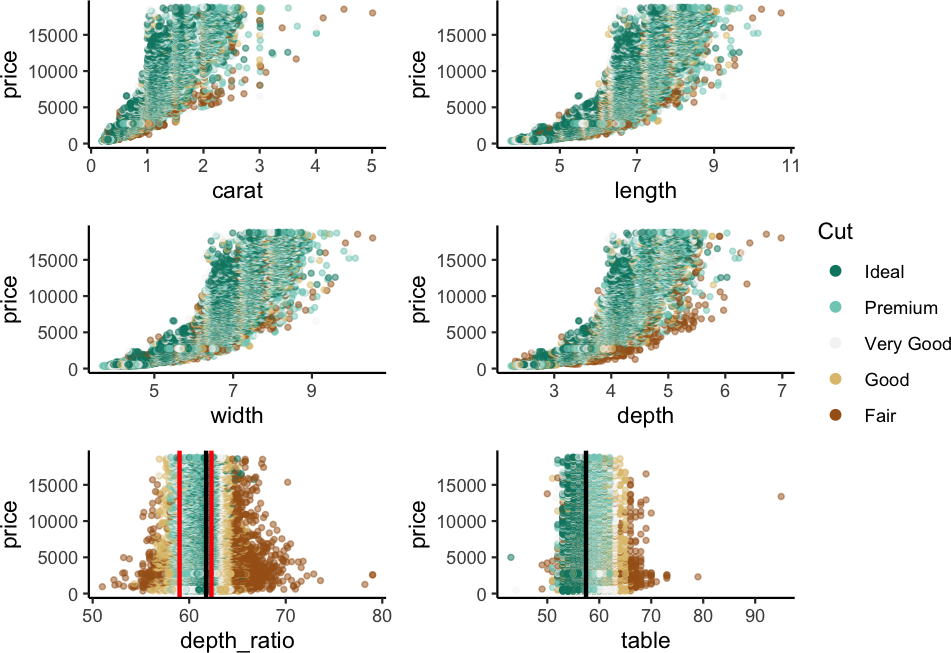
\includegraphics{Diamonds_files/figure-latex/Price by X and Cut-1} \end{center}

\begin{Shaded}
\begin{Highlighting}[]
\CommentTok{\# Correlation between price and quantitative variables}
\NormalTok{price\_correlation }\OtherTok{\textless{}{-}} \FunctionTok{with}\NormalTok{(diamonds,}
     \FunctionTok{data.frame}\NormalTok{(}\AttributeTok{cor\_length\_price =} \FunctionTok{cor}\NormalTok{(length, price), }\AttributeTok{cor\_width\_price =} \FunctionTok{cor}\NormalTok{(width, price), }\AttributeTok{cor\_depth\_price =} \FunctionTok{cor}\NormalTok{(depth, price), }\AttributeTok{cor\_depth\_ratio\_price =} \FunctionTok{cor}\NormalTok{(depth\_ratio, price), }\AttributeTok{cor\_table\_price2 =} \FunctionTok{cor}\NormalTok{(table, price), }\AttributeTok{cor\_carat\_price3 =} \FunctionTok{cor}\NormalTok{(carat, price)))}

\CommentTok{\# Transpose data and put into kable format}
\NormalTok{transpose }\OtherTok{\textless{}{-}} \FunctionTok{t}\NormalTok{(}\FunctionTok{sort}\NormalTok{(}\FunctionTok{round}\NormalTok{(price\_correlation,}\DecValTok{4}\NormalTok{),}\AttributeTok{decreasing =} \ConstantTok{FALSE}\NormalTok{))}
\NormalTok{kable\_corr }\OtherTok{\textless{}{-}} \FunctionTok{kable}\NormalTok{(transpose) }\SpecialCharTok{\%\textgreater{}\%} \FunctionTok{kable\_classic}\NormalTok{() }
\NormalTok{kable\_corr}
\end{Highlighting}
\end{Shaded}

\begin{table}
\centering
\begin{tabular}{l|r}
\hline
cor\_depth\_ratio\_price & -0.0104\\
\hline
cor\_table\_price2 & 0.1273\\
\hline
cor\_depth\_price & 0.8829\\
\hline
cor\_length\_price & 0.8876\\
\hline
cor\_width\_price & 0.8892\\
\hline
cor\_carat\_price3 & 0.9218\\
\hline
\end{tabular}
\end{table}

\hypertarget{variable-visualisation}{%
\subsection{Variable Visualisation}\label{variable-visualisation}}

\begin{Shaded}
\begin{Highlighting}[]
\FunctionTok{ggplot}\NormalTok{(}\FunctionTok{gather}\NormalTok{(}\AttributeTok{data =}\NormalTok{ diamonds[, }\FunctionTok{c}\NormalTok{(}\DecValTok{1}\NormalTok{, }\DecValTok{5}\SpecialCharTok{:}\DecValTok{10}\NormalTok{)]), }\FunctionTok{aes}\NormalTok{(value)) }\SpecialCharTok{+}
  \FunctionTok{geom\_histogram}\NormalTok{(}\FunctionTok{aes}\NormalTok{(}\AttributeTok{y =} \FunctionTok{after\_stat}\NormalTok{(density)),}
                 \AttributeTok{bins =} \DecValTok{10}\NormalTok{,}
                 \AttributeTok{color =} \StringTok{"white"}\NormalTok{,}
                 \AttributeTok{fill =} \StringTok{"\#D8B365"}\NormalTok{) }\SpecialCharTok{+} \CommentTok{\# Creates bin sizing and sets the lines as white}
  \FunctionTok{geom\_density}\NormalTok{(}\AttributeTok{alpha =}\NormalTok{ .}\DecValTok{2}\NormalTok{, }\AttributeTok{fill =} \StringTok{"\#D8B365"}\NormalTok{) }\SpecialCharTok{+}
  \FunctionTok{facet\_wrap}\NormalTok{(}\SpecialCharTok{\textasciitilde{}}\NormalTok{ key, }\AttributeTok{scales =} \StringTok{"free"}\NormalTok{) }\SpecialCharTok{+} \CommentTok{\# Converting the graphs into panels}
  \FunctionTok{ggtitle}\NormalTok{(}\StringTok{"Quantitative Variable Analysis"}\NormalTok{) }\SpecialCharTok{+} \CommentTok{\# Title name}
  \FunctionTok{ylab}\NormalTok{(}\StringTok{"Count"}\NormalTok{) }\SpecialCharTok{+} \FunctionTok{xlab}\NormalTok{(}\StringTok{"Value"}\NormalTok{) }\SpecialCharTok{+} \CommentTok{\# Label names}
  \FunctionTok{theme\_classic}\NormalTok{() }\CommentTok{\# A classic theme, with x and y axis lines and no grid lines}
\end{Highlighting}
\end{Shaded}

\begin{center}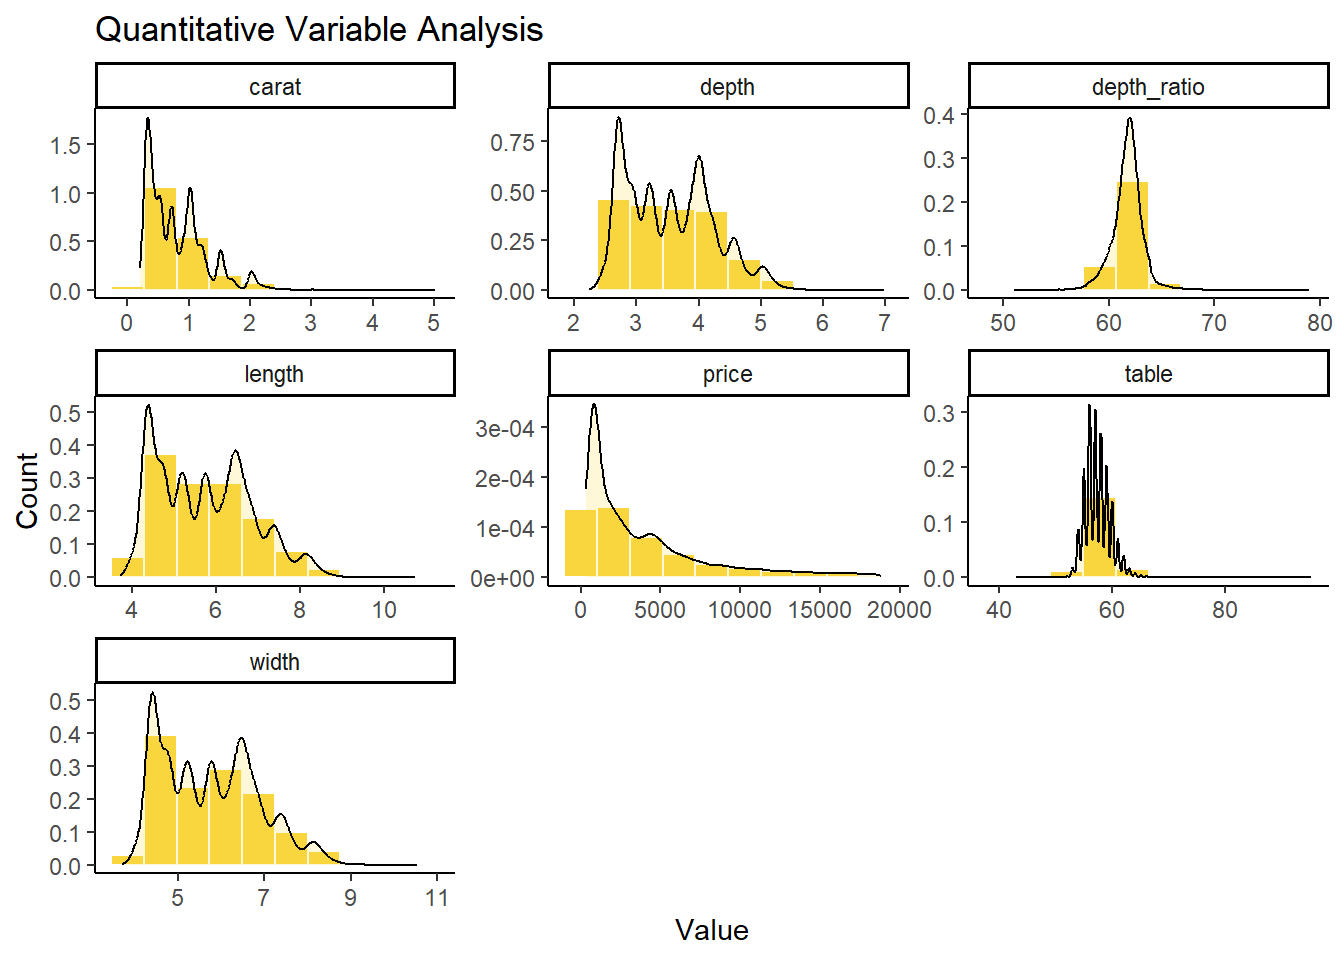
\includegraphics{Diamonds_files/figure-latex/Histograms-1} \end{center}

\begin{Shaded}
\begin{Highlighting}[]
\CommentTok{\# Create heatmap to show variable correlation}
\CommentTok{\# Round the correlation coefficient to two decimal places}
\NormalTok{cormat }\OtherTok{\textless{}{-}} \FunctionTok{round}\NormalTok{(}\FunctionTok{cor}\NormalTok{(diamonds[, }\FunctionTok{c}\NormalTok{(}\DecValTok{1}\NormalTok{, }\DecValTok{5}\SpecialCharTok{:}\DecValTok{10}\NormalTok{)]), }\DecValTok{2}\NormalTok{)}

\CommentTok{\# Use correlation between variables as distance}
\NormalTok{reorder\_cormat }\OtherTok{\textless{}{-}} \ControlFlowTok{function}\NormalTok{(cormat)\{ }
\NormalTok{dd }\OtherTok{\textless{}{-}} \FunctionTok{as.dist}\NormalTok{((}\DecValTok{1}\SpecialCharTok{{-}}\NormalTok{cormat)}\SpecialCharTok{/}\DecValTok{2}\NormalTok{)}
\NormalTok{hc }\OtherTok{\textless{}{-}} \FunctionTok{hclust}\NormalTok{(dd)}
\NormalTok{cormat }\OtherTok{\textless{}{-}}\NormalTok{cormat[hc}\SpecialCharTok{$}\NormalTok{order, hc}\SpecialCharTok{$}\NormalTok{order]}
\FunctionTok{return}\NormalTok{(cormat)}
\NormalTok{\}}

\CommentTok{\# Reorder the correlation matrix}
\NormalTok{cormat }\OtherTok{\textless{}{-}} \FunctionTok{reorder\_cormat}\NormalTok{(cormat)}

\CommentTok{\# Keeping only upper triangular matrix}
\CommentTok{\# upper\_tri returns TRUE/FALSE for each coordinate (TRUE {-}\textgreater{} part of upper triangle)}
\CommentTok{\# multiplying will thus keep the upper triangle values and set the others to 0}
\NormalTok{cormat }\OtherTok{\textless{}{-}}\NormalTok{ cormat}\SpecialCharTok{*}\FunctionTok{upper.tri}\NormalTok{(cormat, }\AttributeTok{diag =} \ConstantTok{TRUE}\NormalTok{)}
\CommentTok{\# Values of the lower triangle (0) are replaced by NA}
\NormalTok{cormat[cormat }\SpecialCharTok{==} \DecValTok{0}\NormalTok{] }\OtherTok{\textless{}{-}} \ConstantTok{NA}

\CommentTok{\# Melt the correlation matrix}
\NormalTok{cormat }\OtherTok{\textless{}{-}}\NormalTok{ reshape2}\SpecialCharTok{::}\FunctionTok{melt}\NormalTok{(cormat, }\AttributeTok{na.rm =} \ConstantTok{TRUE}\NormalTok{)}

\CommentTok{\# Create a ggheatmap with multiple characteristics }
\FunctionTok{ggplot}\NormalTok{(cormat, }\FunctionTok{aes}\NormalTok{(Var2, Var1, }\AttributeTok{fill =}\NormalTok{ value)) }\SpecialCharTok{+}
  \FunctionTok{geom\_tile}\NormalTok{(}\AttributeTok{color =} \StringTok{"white"}\NormalTok{) }\SpecialCharTok{+}
  \FunctionTok{scale\_fill\_gradient2}\NormalTok{(}\AttributeTok{low =} \StringTok{"\#D8B365"}\NormalTok{, }\AttributeTok{high =} \StringTok{"\#15DDD8"}\NormalTok{, }\AttributeTok{mid =} \StringTok{"white"}\NormalTok{,}
                       \AttributeTok{midpoint =} \DecValTok{0}\NormalTok{, }\AttributeTok{limit =} \FunctionTok{c}\NormalTok{(}\SpecialCharTok{{-}}\DecValTok{1}\NormalTok{,}\DecValTok{1}\NormalTok{), }\AttributeTok{space =} \StringTok{"Lab"}\NormalTok{, }\AttributeTok{name=}\StringTok{"Pearson}\SpecialCharTok{\textbackslash{}n}\StringTok{Correlation"}\NormalTok{) }\SpecialCharTok{+}
  \FunctionTok{ggtitle}\NormalTok{(}\StringTok{"Correlation Heatmap"}\NormalTok{) }\SpecialCharTok{+} \CommentTok{\# Title name}
  \FunctionTok{theme\_minimal}\NormalTok{() }\SpecialCharTok{+} \CommentTok{\# Minimal theme, keeps in the lines}
  \FunctionTok{theme}\NormalTok{(}\AttributeTok{axis.text.x =} \FunctionTok{element\_text}\NormalTok{(}\AttributeTok{angle =} \DecValTok{45}\NormalTok{, }\AttributeTok{vjust =} \DecValTok{1}\NormalTok{, }\AttributeTok{size =} \DecValTok{12}\NormalTok{, }\AttributeTok{hjust =} \DecValTok{1}\NormalTok{)) }\SpecialCharTok{+}
  \FunctionTok{coord\_fixed}\NormalTok{() }\SpecialCharTok{+}
  \FunctionTok{geom\_text}\NormalTok{(}\FunctionTok{aes}\NormalTok{(Var2, Var1, }\AttributeTok{label =}\NormalTok{ value), }\AttributeTok{color =} \StringTok{"black"}\NormalTok{, }\AttributeTok{size =} \DecValTok{2}\NormalTok{)}
\end{Highlighting}
\end{Shaded}

\begin{center}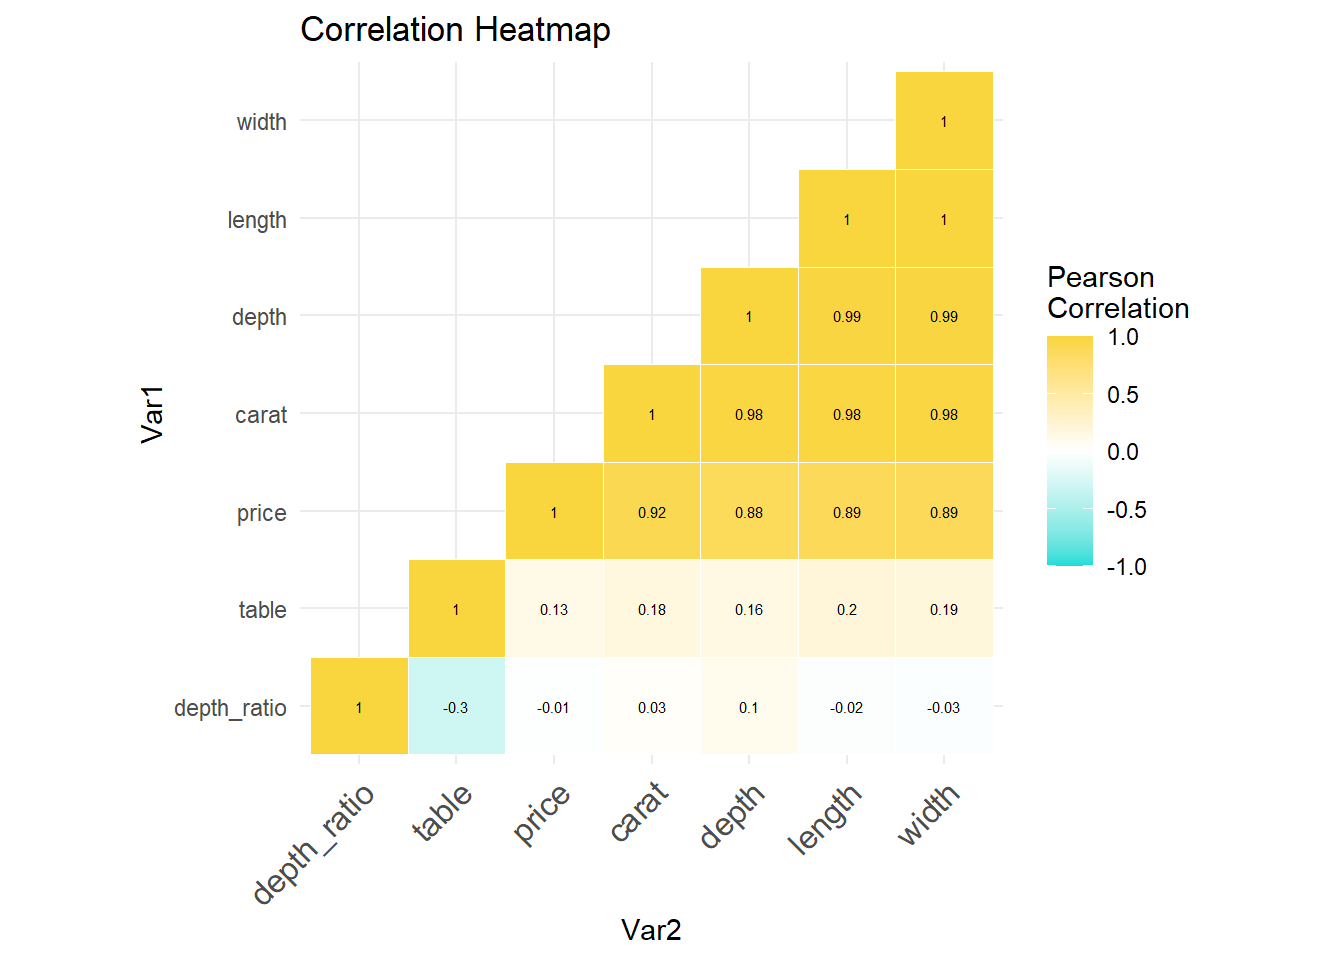
\includegraphics{Diamonds_files/figure-latex/Correlation-1} \end{center}

\begin{Shaded}
\begin{Highlighting}[]
\FunctionTok{rm}\NormalTok{(cormat, reorder\_cormat)}
\end{Highlighting}
\end{Shaded}

\begin{Shaded}
\begin{Highlighting}[]
\CommentTok{\#plot Correlation ellipses}
\FunctionTok{plotcorr}\NormalTok{(}\FunctionTok{cor}\NormalTok{(diamonds[, }\SpecialCharTok{{-}}\FunctionTok{c}\NormalTok{(}\DecValTok{2}\SpecialCharTok{:}\DecValTok{4}\NormalTok{)]), }\AttributeTok{col =} \StringTok{"\#D8B365"}\NormalTok{,}
         \AttributeTok{main =} \StringTok{"Pearson correlation ellipses for numerical variables"}\NormalTok{)}
\end{Highlighting}
\end{Shaded}

\begin{center}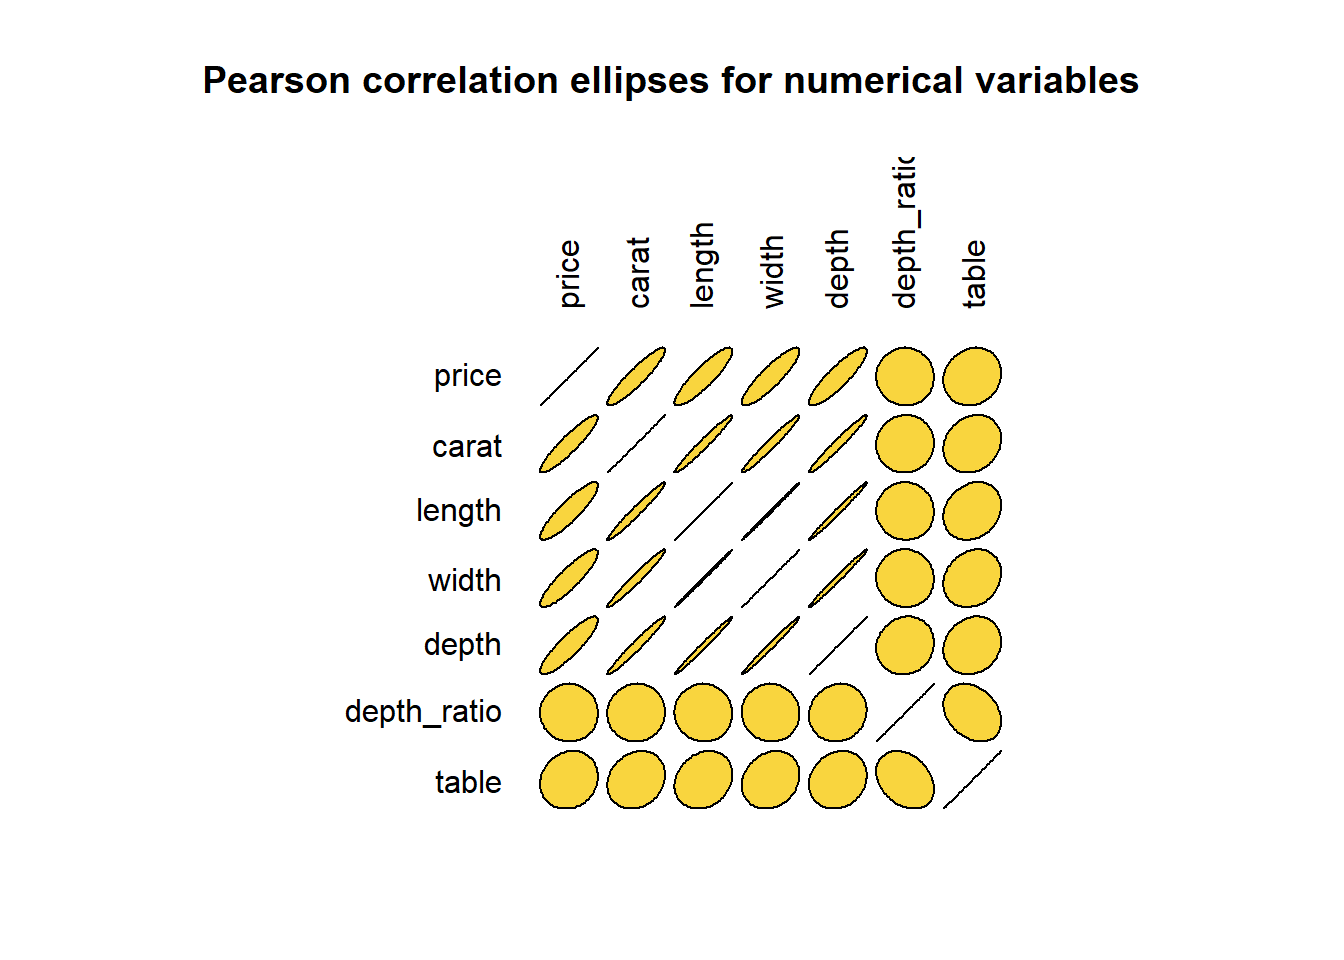
\includegraphics{Diamonds_files/figure-latex/Correlation Plot-1} \end{center}

\begin{Shaded}
\begin{Highlighting}[]
\CommentTok{\# set seed for reproducing the partition}
\FunctionTok{set.seed}\NormalTok{(}\DecValTok{111}\NormalTok{)}

\CommentTok{\# generating training set index}
\NormalTok{train.index }\OtherTok{\textless{}{-}} \FunctionTok{sample}\NormalTok{(}\FunctionTok{c}\NormalTok{(}\DecValTok{1}\SpecialCharTok{:}\FunctionTok{nrow}\NormalTok{(diamonds)), }\FloatTok{0.5}\SpecialCharTok{*}\FunctionTok{nrow}\NormalTok{(diamonds))}

\CommentTok{\# generating validation set index taken from the complementary of training set}
\NormalTok{valid.index }\OtherTok{\textless{}{-}} \FunctionTok{sample}\NormalTok{(}\FunctionTok{setdiff}\NormalTok{(}\FunctionTok{c}\NormalTok{(}\DecValTok{1}\SpecialCharTok{:}\FunctionTok{nrow}\NormalTok{(diamonds)), train.index), }\FloatTok{0.3}\SpecialCharTok{*}\FunctionTok{nrow}\NormalTok{(diamonds))}

\CommentTok{\# defining test set index as complementary of (train.index + valid.index)}
\NormalTok{test.index }\OtherTok{\textless{}{-}} \FunctionTok{as.numeric}\NormalTok{(}\FunctionTok{setdiff}\NormalTok{(}\FunctionTok{row.names}\NormalTok{(diamonds), }\FunctionTok{union}\NormalTok{(train.index, valid.index)))}

\CommentTok{\# creating data tables Train, Valid and Test using the indexes}
\NormalTok{Train }\OtherTok{\textless{}{-}}\NormalTok{ diamonds[train.index, ]}
\NormalTok{Valid }\OtherTok{\textless{}{-}}\NormalTok{ diamonds[valid.index, ]}
\NormalTok{Test }\OtherTok{\textless{}{-}}\NormalTok{ diamonds[test.index, ]}
\end{Highlighting}
\end{Shaded}

\hypertarget{variable-prediction-and-model-performance-evaluation}{%
\section{Variable Prediction and Model Performance
Evaluation}\label{variable-prediction-and-model-performance-evaluation}}

\hypertarget{linear-regression}{%
\subsection{Linear Regression}\label{linear-regression}}

\begin{Shaded}
\begin{Highlighting}[]
\NormalTok{Train\_lr }\OtherTok{\textless{}{-}}\NormalTok{ diamonds[train.index, ]}
\NormalTok{Valid\_lr }\OtherTok{\textless{}{-}}\NormalTok{ diamonds[valid.index, ]}
\NormalTok{Test\_lr  }\OtherTok{\textless{}{-}}\NormalTok{ diamonds[ test.index, ]}
\end{Highlighting}
\end{Shaded}

\begin{Shaded}
\begin{Highlighting}[]
\FunctionTok{VIF}\NormalTok{(}\AttributeTok{y =}\NormalTok{ diamonds}\SpecialCharTok{$}\NormalTok{price, }\AttributeTok{matx =}\NormalTok{ diamonds[, }\SpecialCharTok{{-}}\FunctionTok{c}\NormalTok{(}\DecValTok{1}\NormalTok{)])}
\end{Highlighting}
\end{Shaded}

\begin{verbatim}
##
##                   GVIF Df GVIF^(1/(2*Df))
## cut            2.45522  4         1.11882
## color          1.18398  6         1.01417
## clarity        1.36848  7         1.02266
## carat         25.91780  1         5.09095
## length      1091.42000  1        33.03670
## width       1143.44000  1        33.81480
## depth       2008.33000  1        44.81440
## depth_ratio   31.99350  1         5.65628
## table          1.80396  1         1.34311
##
##   Mean: 165.105
\end{verbatim}

\begin{Shaded}
\begin{Highlighting}[]
\FunctionTok{VIF}\NormalTok{(}\AttributeTok{y =}\NormalTok{ diamonds}\SpecialCharTok{$}\NormalTok{price, }\AttributeTok{matx =}\NormalTok{ diamonds[, }\SpecialCharTok{{-}}\FunctionTok{c}\NormalTok{(}\DecValTok{1}\NormalTok{, }\DecValTok{6}\NormalTok{, }\DecValTok{7}\NormalTok{, }\DecValTok{8}\NormalTok{)])}
\end{Highlighting}
\end{Shaded}

\begin{verbatim}
##
##                GVIF Df GVIF^(1/(2*Df))
## cut         1.93382  4         1.08593
## color       1.17045  6         1.01320
## clarity     1.30388  7         1.01913
## carat       1.32381  1         1.15057
## depth_ratio 1.38914  1         1.17862
## table       1.79505  1         1.33980
##
##   Mean: 1.98352
\end{verbatim}

\begin{Shaded}
\begin{Highlighting}[]
\FunctionTok{plotcorr}\NormalTok{(}\FunctionTok{cor}\NormalTok{(diamonds[, }\SpecialCharTok{{-}}\FunctionTok{c}\NormalTok{(}\DecValTok{2}\SpecialCharTok{:}\DecValTok{4}\NormalTok{, }\DecValTok{6}\SpecialCharTok{:}\DecValTok{8}\NormalTok{)]), }\AttributeTok{col =} \StringTok{"\#D8B365"}\NormalTok{,}
         \AttributeTok{main =} \StringTok{"Pearson correlation ellipses for numerical variables"}\NormalTok{)}
\end{Highlighting}
\end{Shaded}

\begin{center}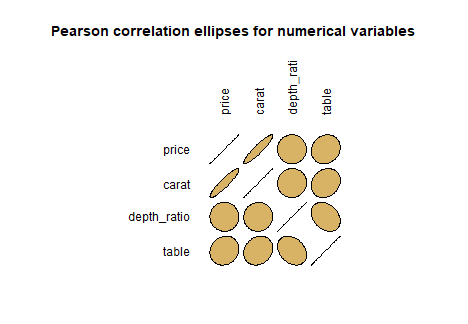
\includegraphics{Diamonds_files/figure-latex/vif-1} \end{center}

\begin{Shaded}
\begin{Highlighting}[]
\FunctionTok{sapply}\NormalTok{(Train\_lr[, }\FunctionTok{c}\NormalTok{(}\DecValTok{1}\NormalTok{, }\DecValTok{5}\SpecialCharTok{:}\DecValTok{10}\NormalTok{)], skewness)}
\end{Highlighting}
\end{Shaded}

\begin{verbatim}
##       price       carat      length       width       depth depth_ratio
##  1.62597473  1.09675143  0.39846889  0.39220078  0.39210931  0.01824979
##       table
##  0.87288692
\end{verbatim}

\begin{Shaded}
\begin{Highlighting}[]
\NormalTok{Train\_lr}\SpecialCharTok{$}\NormalTok{price }\OtherTok{\textless{}{-}} \FunctionTok{log}\NormalTok{(Train\_lr}\SpecialCharTok{$}\NormalTok{price)}
\NormalTok{Train\_lr}\SpecialCharTok{$}\NormalTok{carat }\OtherTok{\textless{}{-}} \FunctionTok{log}\NormalTok{(Train\_lr}\SpecialCharTok{$}\NormalTok{carat)}
\NormalTok{Train\_lr}\SpecialCharTok{$}\NormalTok{table }\OtherTok{\textless{}{-}} \FunctionTok{log}\NormalTok{(Train\_lr}\SpecialCharTok{$}\NormalTok{table)}
\FunctionTok{sapply}\NormalTok{(Train\_lr[, }\FunctionTok{c}\NormalTok{(}\DecValTok{1}\NormalTok{, }\DecValTok{5}\SpecialCharTok{:}\DecValTok{10}\NormalTok{)], skewness)}
\end{Highlighting}
\end{Shaded}

\begin{verbatim}
##       price       carat      length       width       depth depth_ratio
##  0.11305083  0.09668960  0.39846889  0.39220078  0.39210931  0.01824979
##       table
##  0.64541910
\end{verbatim}

\begin{Shaded}
\begin{Highlighting}[]
\NormalTok{Valid\_lr}\SpecialCharTok{$}\NormalTok{price }\OtherTok{\textless{}{-}} \FunctionTok{log}\NormalTok{(Valid\_lr}\SpecialCharTok{$}\NormalTok{price)}
\NormalTok{Valid\_lr}\SpecialCharTok{$}\NormalTok{carat }\OtherTok{\textless{}{-}} \FunctionTok{log}\NormalTok{(Valid\_lr}\SpecialCharTok{$}\NormalTok{carat)}
\NormalTok{Valid\_lr}\SpecialCharTok{$}\NormalTok{table }\OtherTok{\textless{}{-}} \FunctionTok{log}\NormalTok{(Valid\_lr}\SpecialCharTok{$}\NormalTok{table)}
\end{Highlighting}
\end{Shaded}

\begin{Shaded}
\begin{Highlighting}[]
\FunctionTok{ggplot}\NormalTok{(}\FunctionTok{gather}\NormalTok{(}\AttributeTok{data =}\NormalTok{ Train\_lr[, }\FunctionTok{c}\NormalTok{(}\DecValTok{1}\NormalTok{, }\DecValTok{5}\SpecialCharTok{:}\DecValTok{10}\NormalTok{)]), }\FunctionTok{aes}\NormalTok{(value)) }\SpecialCharTok{+}
  \FunctionTok{geom\_histogram}\NormalTok{(}\FunctionTok{aes}\NormalTok{(}\AttributeTok{y =} \FunctionTok{after\_stat}\NormalTok{(density)),}
                 \AttributeTok{color =} \StringTok{"white"}\NormalTok{,}
                 \AttributeTok{fill =} \StringTok{"\#D8B365"}\NormalTok{) }\SpecialCharTok{+}             \CommentTok{\# Creates bin sizing with colors}
  \FunctionTok{geom\_density}\NormalTok{(}\AttributeTok{alpha =}\NormalTok{ .}\DecValTok{2}\NormalTok{, }\AttributeTok{fill =} \StringTok{"\#D8B365"}\NormalTok{) }\SpecialCharTok{+}
  \FunctionTok{facet\_wrap}\NormalTok{(}\SpecialCharTok{\textasciitilde{}}\NormalTok{ key, }\AttributeTok{scales =} \StringTok{"free"}\NormalTok{) }\SpecialCharTok{+}           \CommentTok{\# Converting the graphs into panels}
  \FunctionTok{ggtitle}\NormalTok{(}\StringTok{"Histograms of numerical variables"}\NormalTok{) }\SpecialCharTok{+} \CommentTok{\# Title name}
  \FunctionTok{ylab}\NormalTok{(}\StringTok{"Count"}\NormalTok{) }\SpecialCharTok{+} \FunctionTok{xlab}\NormalTok{(}\StringTok{"Value"}\NormalTok{) }\SpecialCharTok{+}                \CommentTok{\# Label names}
  \FunctionTok{theme\_classic}\NormalTok{()                                }\CommentTok{\# Theme with x and y axis lines and no grid lines}
\end{Highlighting}
\end{Shaded}

\begin{center}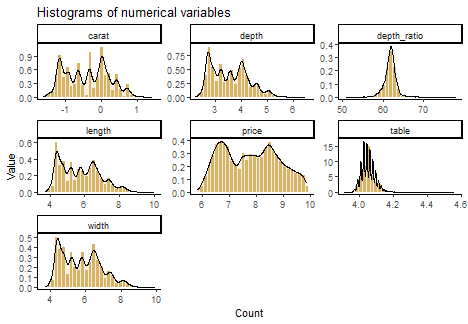
\includegraphics{Diamonds_files/figure-latex/hist-unskewed-1} \end{center}

\begin{Shaded}
\begin{Highlighting}[]
\NormalTok{norm.values }\OtherTok{\textless{}{-}} \FunctionTok{preProcess}\NormalTok{(Train\_lr[, }\FunctionTok{c}\NormalTok{(}\DecValTok{1}\NormalTok{, }\DecValTok{5}\SpecialCharTok{:}\DecValTok{10}\NormalTok{)], }\AttributeTok{method=}\FunctionTok{c}\NormalTok{(}\StringTok{"center"}\NormalTok{, }\StringTok{"scale"}\NormalTok{))}

\NormalTok{Train\_lr[, }\FunctionTok{c}\NormalTok{(}\DecValTok{1}\NormalTok{, }\DecValTok{5}\SpecialCharTok{:}\DecValTok{10}\NormalTok{)] }\OtherTok{\textless{}{-}} \FunctionTok{predict}\NormalTok{(norm.values, Train\_lr[, }\FunctionTok{c}\NormalTok{(}\DecValTok{1}\NormalTok{, }\DecValTok{5}\SpecialCharTok{:}\DecValTok{10}\NormalTok{)])}
\NormalTok{Valid\_lr[, }\FunctionTok{c}\NormalTok{(}\DecValTok{1}\NormalTok{, }\DecValTok{5}\SpecialCharTok{:}\DecValTok{10}\NormalTok{)] }\OtherTok{\textless{}{-}} \FunctionTok{predict}\NormalTok{(norm.values, Valid\_lr[, }\FunctionTok{c}\NormalTok{(}\DecValTok{1}\NormalTok{, }\DecValTok{5}\SpecialCharTok{:}\DecValTok{10}\NormalTok{)])}
\NormalTok{ Test\_lr[, }\FunctionTok{c}\NormalTok{(}\DecValTok{1}\NormalTok{, }\DecValTok{5}\SpecialCharTok{:}\DecValTok{10}\NormalTok{)] }\OtherTok{\textless{}{-}} \FunctionTok{predict}\NormalTok{(norm.values,  Test\_lr[, }\FunctionTok{c}\NormalTok{(}\DecValTok{1}\NormalTok{, }\DecValTok{5}\SpecialCharTok{:}\DecValTok{10}\NormalTok{)])}
\end{Highlighting}
\end{Shaded}

\begin{Shaded}
\begin{Highlighting}[]
\NormalTok{LM\_complete }\OtherTok{=} \FunctionTok{lm}\NormalTok{(price }\SpecialCharTok{\textasciitilde{}}\NormalTok{. , }\AttributeTok{data =}\NormalTok{ Train\_lr)}
\FunctionTok{summary}\NormalTok{(LM\_complete)}
\end{Highlighting}
\end{Shaded}

\begin{verbatim}
##
## Call:
## lm(formula = price ~ ., data = Train_lr)
##
## Residuals:
##      Min       1Q   Median       3Q      Max
## -1.04059 -0.08291  0.00028  0.08156  1.42487
##
## Coefficients:
##               Estimate Std. Error t value             Pr(>|t|)
## (Intercept) -0.0747373  0.0016289 -45.882 < 0.0000000000000002 ***
## cut.L        0.1168565  0.0037189  31.422 < 0.0000000000000002 ***
## cut.Q       -0.0342102  0.0030248 -11.310 < 0.0000000000000002 ***
## cut.C        0.0174498  0.0027023   6.457      0.0000000001084 ***
## cut^4        0.0003697  0.0020867   0.177              0.85937
## color.L      0.4366728  0.0028463 153.417 < 0.0000000000000002 ***
## color.Q     -0.0974458  0.0025856 -37.687 < 0.0000000000000002 ***
## color.C      0.0126123  0.0024180   5.216      0.0000001841568 ***
## color^4      0.0134193  0.0022210   6.042      0.0000000015434 ***
## color^5      0.0001336  0.0021044   0.063              0.94940
## color^6      0.0026592  0.0019108   1.392              0.16404
## clarity.L    0.9080235  0.0050105 181.224 < 0.0000000000000002 ***
## clarity.Q   -0.2486235  0.0046594 -53.360 < 0.0000000000000002 ***
## clarity.C    0.1370069  0.0039810  34.415 < 0.0000000000000002 ***
## clarity^4   -0.0685371  0.0031777 -21.568 < 0.0000000000000002 ***
## clarity^5    0.0290689  0.0025896  11.225 < 0.0000000000000002 ***
## clarity^6   -0.0022942  0.0022444  -1.022              0.30670
## clarity^7    0.0312779  0.0019833  15.771 < 0.0000000000000002 ***
## carat        0.9997686  0.0082204 121.621 < 0.0000000000000002 ***
## length       0.1775342  0.0266043   6.673      0.0000000000255 ***
## width       -0.0200231  0.0270778  -0.739              0.45963
## depth       -0.0702733  0.0359774  -1.953              0.05080 .
## depth_ratio  0.0117907  0.0045226   2.607              0.00914 **
## table        0.0011885  0.0010849   1.096              0.27330
## ---
## Signif. codes:  0 '***' 0.001 '**' 0.01 '*' 0.05 '.' 0.1 ' ' 1
##
## Residual standard error: 0.131 on 26808 degrees of freedom
## Multiple R-squared:  0.9829, Adjusted R-squared:  0.9828
## F-statistic: 6.685e+04 on 23 and 26808 DF,  p-value: < 0.00000000000000022
\end{verbatim}

\begin{Shaded}
\begin{Highlighting}[]
\NormalTok{LM\_forward\_complete }\OtherTok{=} \FunctionTok{step}\NormalTok{(LM\_complete, }\AttributeTok{direction =} \StringTok{"forward"}\NormalTok{)}
\end{Highlighting}
\end{Shaded}

\begin{verbatim}
## Start:  AIC=-109064.2
## price ~ cut + color + clarity + carat + length + width + depth +
##     depth_ratio + table
\end{verbatim}

\begin{Shaded}
\begin{Highlighting}[]
\FunctionTok{summary}\NormalTok{(LM\_forward\_complete)    }\CommentTok{\# no selection}
\end{Highlighting}
\end{Shaded}

\begin{verbatim}
##
## Call:
## lm(formula = price ~ cut + color + clarity + carat + length +
##     width + depth + depth_ratio + table, data = Train_lr)
##
## Residuals:
##      Min       1Q   Median       3Q      Max
## -1.04059 -0.08291  0.00028  0.08156  1.42487
##
## Coefficients:
##               Estimate Std. Error t value             Pr(>|t|)
## (Intercept) -0.0747373  0.0016289 -45.882 < 0.0000000000000002 ***
## cut.L        0.1168565  0.0037189  31.422 < 0.0000000000000002 ***
## cut.Q       -0.0342102  0.0030248 -11.310 < 0.0000000000000002 ***
## cut.C        0.0174498  0.0027023   6.457      0.0000000001084 ***
## cut^4        0.0003697  0.0020867   0.177              0.85937
## color.L      0.4366728  0.0028463 153.417 < 0.0000000000000002 ***
## color.Q     -0.0974458  0.0025856 -37.687 < 0.0000000000000002 ***
## color.C      0.0126123  0.0024180   5.216      0.0000001841568 ***
## color^4      0.0134193  0.0022210   6.042      0.0000000015434 ***
## color^5      0.0001336  0.0021044   0.063              0.94940
## color^6      0.0026592  0.0019108   1.392              0.16404
## clarity.L    0.9080235  0.0050105 181.224 < 0.0000000000000002 ***
## clarity.Q   -0.2486235  0.0046594 -53.360 < 0.0000000000000002 ***
## clarity.C    0.1370069  0.0039810  34.415 < 0.0000000000000002 ***
## clarity^4   -0.0685371  0.0031777 -21.568 < 0.0000000000000002 ***
## clarity^5    0.0290689  0.0025896  11.225 < 0.0000000000000002 ***
## clarity^6   -0.0022942  0.0022444  -1.022              0.30670
## clarity^7    0.0312779  0.0019833  15.771 < 0.0000000000000002 ***
## carat        0.9997686  0.0082204 121.621 < 0.0000000000000002 ***
## length       0.1775342  0.0266043   6.673      0.0000000000255 ***
## width       -0.0200231  0.0270778  -0.739              0.45963
## depth       -0.0702733  0.0359774  -1.953              0.05080 .
## depth_ratio  0.0117907  0.0045226   2.607              0.00914 **
## table        0.0011885  0.0010849   1.096              0.27330
## ---
## Signif. codes:  0 '***' 0.001 '**' 0.01 '*' 0.05 '.' 0.1 ' ' 1
##
## Residual standard error: 0.131 on 26808 degrees of freedom
## Multiple R-squared:  0.9829, Adjusted R-squared:  0.9828
## F-statistic: 6.685e+04 on 23 and 26808 DF,  p-value: < 0.00000000000000022
\end{verbatim}

\begin{Shaded}
\begin{Highlighting}[]
\NormalTok{LM\_backward\_complete }\OtherTok{=} \FunctionTok{step}\NormalTok{(LM\_complete, }\AttributeTok{direction =} \StringTok{"backward"}\NormalTok{)}
\end{Highlighting}
\end{Shaded}

\begin{verbatim}
## Start:  AIC=-109064.2
## price ~ cut + color + clarity + carat + length + width + depth +
##     depth_ratio + table
##
##               Df Sum of Sq     RSS     AIC
## - width        1      0.01  459.84 -109066
## - table        1      0.02  459.85 -109065
## <none>                      459.83 -109064
## - depth        1      0.07  459.89 -109062
## - depth_ratio  1      0.12  459.95 -109059
## - length       1      0.76  460.59 -109022
## - cut          4     19.38  479.21 -107965
## - carat        1    253.72  713.54  -97277
## - color        6    428.53  888.36  -91407
## - clarity      7    874.13 1333.96  -80501
##
## Step:  AIC=-109065.7
## price ~ cut + color + clarity + carat + length + depth + depth_ratio +
##     table
##
##               Df Sum of Sq     RSS     AIC
## - table        1      0.02  459.86 -109066
## <none>                      459.84 -109066
## - depth        1      0.18  460.02 -109057
## - depth_ratio  1      0.30  460.14 -109050
## - length       1      0.75  460.59 -109024
## - cut          4     19.38  479.22 -107966
## - carat        1    256.52  716.35  -97173
## - color        6    428.96  888.80  -91395
## - clarity      7    877.59 1337.43  -80433
##
## Step:  AIC=-109066.4
## price ~ cut + color + clarity + carat + length + depth + depth_ratio
##
##               Df Sum of Sq     RSS     AIC
## <none>                      459.86 -109066
## - depth        1      0.18  460.04 -109058
## - depth_ratio  1      0.29  460.15 -109052
## - length       1      0.75  460.61 -109025
## - cut          4     24.58  484.44 -107677
## - carat        1    261.25  721.11  -96998
## - color        6    429.14  889.00  -91391
## - clarity      7    877.84 1337.70  -80430
\end{verbatim}

\begin{Shaded}
\begin{Highlighting}[]
\FunctionTok{summary}\NormalTok{(LM\_backward\_complete)   }\CommentTok{\# like LM\_CpAIC\_complete}
\end{Highlighting}
\end{Shaded}

\begin{verbatim}
##
## Call:
## lm(formula = price ~ cut + color + clarity + carat + length +
##     depth + depth_ratio, data = Train_lr)
##
## Residuals:
##      Min       1Q   Median       3Q      Max
## -1.04014 -0.08295  0.00025  0.08161  1.42593
##
## Coefficients:
##               Estimate Std. Error t value             Pr(>|t|)
## (Intercept) -0.0741493  0.0015667 -47.329 < 0.0000000000000002 ***
## cut.L        0.1150923  0.0034602  33.262 < 0.0000000000000002 ***
## cut.Q       -0.0339481  0.0029582 -11.476 < 0.0000000000000002 ***
## cut.C        0.0163231  0.0025452   6.413      0.0000000001447 ***
## cut^4       -0.0001739  0.0020487  -0.085              0.93235
## color.L      0.4366337  0.0028441 153.523 < 0.0000000000000002 ***
## color.Q     -0.0974187  0.0025833 -37.711 < 0.0000000000000002 ***
## color.C      0.0125915  0.0024179   5.208      0.0000001927323 ***
## color^4      0.0133674  0.0022204   6.020      0.0000000017651 ***
## color^5      0.0001194  0.0021042   0.057              0.95475
## color^6      0.0026739  0.0019108   1.399              0.16171
## clarity.L    0.9075881  0.0049934 181.757 < 0.0000000000000002 ***
## clarity.Q   -0.2483814  0.0046523 -53.389 < 0.0000000000000002 ***
## clarity.C    0.1367692  0.0039749  34.408 < 0.0000000000000002 ***
## clarity^4   -0.0684754  0.0031760 -21.560 < 0.0000000000000002 ***
## clarity^5    0.0289678  0.0025881  11.193 < 0.0000000000000002 ***
## clarity^6   -0.0022952  0.0022444  -1.023              0.30649
## clarity^7    0.0313111  0.0019831  15.789 < 0.0000000000000002 ***
## carat        1.0002821  0.0081052 123.413 < 0.0000000000000002 ***
## length       0.1751101  0.0264602   6.618      0.0000000000371 ***
## depth       -0.0884193  0.0271461  -3.257              0.00113 **
## depth_ratio  0.0136166  0.0033272   4.093      0.0000427910418 ***
## ---
## Signif. codes:  0 '***' 0.001 '**' 0.01 '*' 0.05 '.' 0.1 ' ' 1
##
## Residual standard error: 0.131 on 26810 degrees of freedom
## Multiple R-squared:  0.9829, Adjusted R-squared:  0.9828
## F-statistic: 7.321e+04 on 21 and 26810 DF,  p-value: < 0.00000000000000022
\end{verbatim}

\begin{Shaded}
\begin{Highlighting}[]
\NormalTok{LM\_stepwise\_complete }\OtherTok{=} \FunctionTok{step}\NormalTok{(LM\_complete, }\AttributeTok{direction =} \StringTok{"both"}\NormalTok{)}
\end{Highlighting}
\end{Shaded}

\begin{verbatim}
## Start:  AIC=-109064.2
## price ~ cut + color + clarity + carat + length + width + depth +
##     depth_ratio + table
##
##               Df Sum of Sq     RSS     AIC
## - width        1      0.01  459.84 -109066
## - table        1      0.02  459.85 -109065
## <none>                      459.83 -109064
## - depth        1      0.07  459.89 -109062
## - depth_ratio  1      0.12  459.95 -109059
## - length       1      0.76  460.59 -109022
## - cut          4     19.38  479.21 -107965
## - carat        1    253.72  713.54  -97277
## - color        6    428.53  888.36  -91407
## - clarity      7    874.13 1333.96  -80501
##
## Step:  AIC=-109065.7
## price ~ cut + color + clarity + carat + length + depth + depth_ratio +
##     table
##
##               Df Sum of Sq     RSS     AIC
## - table        1      0.02  459.86 -109066
## <none>                      459.84 -109066
## + width        1      0.01  459.83 -109064
## - depth        1      0.18  460.02 -109057
## - depth_ratio  1      0.30  460.14 -109050
## - length       1      0.75  460.59 -109024
## - cut          4     19.38  479.22 -107966
## - carat        1    256.52  716.35  -97173
## - color        6    428.96  888.80  -91395
## - clarity      7    877.59 1337.43  -80433
##
## Step:  AIC=-109066.4
## price ~ cut + color + clarity + carat + length + depth + depth_ratio
##
##               Df Sum of Sq     RSS     AIC
## <none>                      459.86 -109066
## + table        1      0.02  459.84 -109066
## + width        1      0.01  459.85 -109065
## - depth        1      0.18  460.04 -109058
## - depth_ratio  1      0.29  460.15 -109052
## - length       1      0.75  460.61 -109025
## - cut          4     24.58  484.44 -107677
## - carat        1    261.25  721.11  -96998
## - color        6    429.14  889.00  -91391
## - clarity      7    877.84 1337.70  -80430
\end{verbatim}

\begin{Shaded}
\begin{Highlighting}[]
\FunctionTok{summary}\NormalTok{(LM\_stepwise\_complete)   }\CommentTok{\# like LM\_CpAIC\_complete}
\end{Highlighting}
\end{Shaded}

\begin{verbatim}
##
## Call:
## lm(formula = price ~ cut + color + clarity + carat + length +
##     depth + depth_ratio, data = Train_lr)
##
## Residuals:
##      Min       1Q   Median       3Q      Max
## -1.04014 -0.08295  0.00025  0.08161  1.42593
##
## Coefficients:
##               Estimate Std. Error t value             Pr(>|t|)
## (Intercept) -0.0741493  0.0015667 -47.329 < 0.0000000000000002 ***
## cut.L        0.1150923  0.0034602  33.262 < 0.0000000000000002 ***
## cut.Q       -0.0339481  0.0029582 -11.476 < 0.0000000000000002 ***
## cut.C        0.0163231  0.0025452   6.413      0.0000000001447 ***
## cut^4       -0.0001739  0.0020487  -0.085              0.93235
## color.L      0.4366337  0.0028441 153.523 < 0.0000000000000002 ***
## color.Q     -0.0974187  0.0025833 -37.711 < 0.0000000000000002 ***
## color.C      0.0125915  0.0024179   5.208      0.0000001927323 ***
## color^4      0.0133674  0.0022204   6.020      0.0000000017651 ***
## color^5      0.0001194  0.0021042   0.057              0.95475
## color^6      0.0026739  0.0019108   1.399              0.16171
## clarity.L    0.9075881  0.0049934 181.757 < 0.0000000000000002 ***
## clarity.Q   -0.2483814  0.0046523 -53.389 < 0.0000000000000002 ***
## clarity.C    0.1367692  0.0039749  34.408 < 0.0000000000000002 ***
## clarity^4   -0.0684754  0.0031760 -21.560 < 0.0000000000000002 ***
## clarity^5    0.0289678  0.0025881  11.193 < 0.0000000000000002 ***
## clarity^6   -0.0022952  0.0022444  -1.023              0.30649
## clarity^7    0.0313111  0.0019831  15.789 < 0.0000000000000002 ***
## carat        1.0002821  0.0081052 123.413 < 0.0000000000000002 ***
## length       0.1751101  0.0264602   6.618      0.0000000000371 ***
## depth       -0.0884193  0.0271461  -3.257              0.00113 **
## depth_ratio  0.0136166  0.0033272   4.093      0.0000427910418 ***
## ---
## Signif. codes:  0 '***' 0.001 '**' 0.01 '*' 0.05 '.' 0.1 ' ' 1
##
## Residual standard error: 0.131 on 26810 degrees of freedom
## Multiple R-squared:  0.9829, Adjusted R-squared:  0.9828
## F-statistic: 7.321e+04 on 21 and 26810 DF,  p-value: < 0.00000000000000022
\end{verbatim}

\begin{Shaded}
\begin{Highlighting}[]
\FunctionTok{options}\NormalTok{(}\AttributeTok{scipen =} \DecValTok{999}\NormalTok{)}
\FunctionTok{GlobalCrit}\NormalTok{(LM\_complete)}
\end{Highlighting}
\end{Shaded}

\begin{verbatim}
##
## -----------------------------------------------------
##   GLOBAL VARIABLE SELECTION PROCEDURE
##
##   ( Data =  Train_lr )
##
##   A = cut
##   B = color
##   C = clarity
##   D = carat
##   E = length
##   F = width
##   G = depth
##   H = depth_ratio
##   I = table
##
##   Models      |  Cp             |  AIC            |
##   -------------------------------------------------
##   ABCDEF      |      2.84  (10) |  32937.47  (10) |
##   ABCDEH      |      2.49  ( 9) |  32937.81  ( 9) |
##   ABCDEFG     |  -   0.63  ( 7) |  32940.94  ( 7) |
##   ABCDEFH     |  -   3.12  ( 5) |  32943.44  ( 5) |
##   ABCDEGH     |  -   6.12  ( 1) |  32946.43  ( 1) |
##   ABCDEFGH    |  -   4.80  ( 3) |  32945.11  ( 3) |
##   ABCDEFGI    |      0.80  ( 8) |  32939.51  ( 8) |
##   ABCDEFHI    |  -   2.18  ( 6) |  32942.50  ( 6) |
##   ABCDEGHI    |  -   5.45  ( 2) |  32945.77  ( 2) |
##   ABCDEFGHI   |  -   3.00  ( 4) |  32944.32  ( 4) |
##
## -----------------------------------------------------
\end{verbatim}

\begin{verbatim}
##
## -----------------------------------------------------
##   GLOBAL VARIABLE SELECTION PROCEDURE
##
##   ( Data =  Train_lr )
##
##   A = cut
##   B = color
##   C = clarity
##   D = carat
##   E = length
##   F = width
##   G = depth
##   H = depth_ratio
##   I = table
##
##   Models      |  Cp             |  AIC            |
##   -------------------------------------------------
##   ABCDEF      |      2.84  (10) |  32937.47  (10) |
##   ABCDEH      |      2.49  ( 9) |  32937.81  ( 9) |
##   ABCDEFG     |  -   0.63  ( 7) |  32940.94  ( 7) |
##   ABCDEFH     |  -   3.12  ( 5) |  32943.44  ( 5) |
##   ABCDEGH     |  -   6.12  ( 1) |  32946.43  ( 1) |
##   ABCDEFGH    |  -   4.80  ( 3) |  32945.11  ( 3) |
##   ABCDEFGI    |      0.80  ( 8) |  32939.51  ( 8) |
##   ABCDEFHI    |  -   2.18  ( 6) |  32942.50  ( 6) |
##   ABCDEGHI    |  -   5.45  ( 2) |  32945.77  ( 2) |
##   ABCDEFGHI   |  -   3.00  ( 4) |  32944.32  ( 4) |
##
## -----------------------------------------------------
\end{verbatim}

\begin{Shaded}
\begin{Highlighting}[]
\NormalTok{LM\_CpAIC\_complete }\OtherTok{=} \FunctionTok{lm}\NormalTok{(price }\SpecialCharTok{\textasciitilde{}}\NormalTok{ . , }\AttributeTok{data =}\NormalTok{ Train\_lr[, }\FunctionTok{c}\NormalTok{(}\DecValTok{1}\SpecialCharTok{:}\DecValTok{6}\NormalTok{, }\DecValTok{8}\NormalTok{, }\DecValTok{9}\NormalTok{)])}
\FunctionTok{summary}\NormalTok{(LM\_CpAIC\_complete)}
\end{Highlighting}
\end{Shaded}

\begin{verbatim}
##
## Call:
## lm(formula = price ~ ., data = Train_lr[, c(1:6, 8, 9)])
##
## Residuals:
##      Min       1Q   Median       3Q      Max
## -1.04014 -0.08295  0.00025  0.08161  1.42593
##
## Coefficients:
##               Estimate Std. Error t value             Pr(>|t|)
## (Intercept) -0.0741493  0.0015667 -47.329 < 0.0000000000000002 ***
## cut.L        0.1150923  0.0034602  33.262 < 0.0000000000000002 ***
## cut.Q       -0.0339481  0.0029582 -11.476 < 0.0000000000000002 ***
## cut.C        0.0163231  0.0025452   6.413      0.0000000001447 ***
## cut^4       -0.0001739  0.0020487  -0.085              0.93235
## color.L      0.4366337  0.0028441 153.523 < 0.0000000000000002 ***
## color.Q     -0.0974187  0.0025833 -37.711 < 0.0000000000000002 ***
## color.C      0.0125915  0.0024179   5.208      0.0000001927323 ***
## color^4      0.0133674  0.0022204   6.020      0.0000000017651 ***
## color^5      0.0001194  0.0021042   0.057              0.95475
## color^6      0.0026739  0.0019108   1.399              0.16171
## clarity.L    0.9075881  0.0049934 181.757 < 0.0000000000000002 ***
## clarity.Q   -0.2483814  0.0046523 -53.389 < 0.0000000000000002 ***
## clarity.C    0.1367692  0.0039749  34.408 < 0.0000000000000002 ***
## clarity^4   -0.0684754  0.0031760 -21.560 < 0.0000000000000002 ***
## clarity^5    0.0289678  0.0025881  11.193 < 0.0000000000000002 ***
## clarity^6   -0.0022952  0.0022444  -1.023              0.30649
## clarity^7    0.0313111  0.0019831  15.789 < 0.0000000000000002 ***
## carat        1.0002821  0.0081052 123.413 < 0.0000000000000002 ***
## length       0.1751101  0.0264602   6.618      0.0000000000371 ***
## depth       -0.0884193  0.0271461  -3.257              0.00113 **
## depth_ratio  0.0136166  0.0033272   4.093      0.0000427910418 ***
## ---
## Signif. codes:  0 '***' 0.001 '**' 0.01 '*' 0.05 '.' 0.1 ' ' 1
##
## Residual standard error: 0.131 on 26810 degrees of freedom
## Multiple R-squared:  0.9829, Adjusted R-squared:  0.9828
## F-statistic: 7.321e+04 on 21 and 26810 DF,  p-value: < 0.00000000000000022
\end{verbatim}

\begin{Shaded}
\begin{Highlighting}[]
\NormalTok{Train\_minus\_corr }\OtherTok{\textless{}{-}}\NormalTok{ Train\_lr[, }\SpecialCharTok{{-}}\FunctionTok{c}\NormalTok{(}\DecValTok{6}\SpecialCharTok{:}\DecValTok{8}\NormalTok{)]}
\NormalTok{LM\_minus\_corr }\OtherTok{=} \FunctionTok{lm}\NormalTok{(price }\SpecialCharTok{\textasciitilde{}}\NormalTok{ ., }\AttributeTok{data =}\NormalTok{ Train\_minus\_corr)}
\FunctionTok{summary}\NormalTok{(LM\_minus\_corr)}
\end{Highlighting}
\end{Shaded}

\begin{verbatim}
##
## Call:
## lm(formula = price ~ ., data = Train_minus_corr)
##
## Residuals:
##      Min       1Q   Median       3Q      Max
## -0.98683 -0.08456 -0.00054  0.08206  1.42888
##
## Coefficients:
##               Estimate Std. Error  t value             Pr(>|t|)
## (Intercept) -0.0733380  0.0016248  -45.136 < 0.0000000000000002 ***
## cut.L        0.1174782  0.0037111   31.656 < 0.0000000000000002 ***
## cut.Q       -0.0331237  0.0029650  -11.172 < 0.0000000000000002 ***
## cut.C        0.0132619  0.0025653    5.170         0.0000002361 ***
## cut^4       -0.0022453  0.0020453   -1.098               0.2723
## color.L      0.4322410  0.0028233  153.096 < 0.0000000000000002 ***
## color.Q     -0.0958030  0.0025851  -37.059 < 0.0000000000000002 ***
## color.C      0.0133140  0.0024238    5.493         0.0000000399 ***
## color^4      0.0125884  0.0022260    5.655         0.0000000157 ***
## color^5     -0.0001023  0.0021099   -0.048               0.9613
## color^6      0.0028366  0.0019160    1.481               0.1388
## clarity.L    0.9068901  0.0050015  181.324 < 0.0000000000000002 ***
## clarity.Q   -0.2447781  0.0046522  -52.615 < 0.0000000000000002 ***
## clarity.C    0.1346227  0.0039816   33.811 < 0.0000000000000002 ***
## clarity^4   -0.0686749  0.0031846  -21.564 < 0.0000000000000002 ***
## clarity^5    0.0288881  0.0025955   11.130 < 0.0000000000000002 ***
## clarity^6   -0.0024999  0.0022505   -1.111               0.2667
## clarity^7    0.0320730  0.0019874   16.138 < 0.0000000000000002 ***
## carat        1.0865804  0.0009254 1174.133 < 0.0000000000000002 ***
## depth_ratio -0.0016945  0.0009461   -1.791               0.0733 .
## table       -0.0001141  0.0010774   -0.106               0.9157
## ---
## Signif. codes:  0 '***' 0.001 '**' 0.01 '*' 0.05 '.' 0.1 ' ' 1
##
## Residual standard error: 0.1313 on 26811 degrees of freedom
## Multiple R-squared:  0.9828, Adjusted R-squared:  0.9828
## F-statistic: 7.644e+04 on 20 and 26811 DF,  p-value: < 0.00000000000000022
\end{verbatim}

\begin{Shaded}
\begin{Highlighting}[]
\NormalTok{LM\_backward\_minus\_corr }\OtherTok{=} \FunctionTok{step}\NormalTok{(LM\_minus\_corr, }\AttributeTok{direction =} \StringTok{"backward"}\NormalTok{)}
\end{Highlighting}
\end{Shaded}

\begin{verbatim}
## Start:  AIC=-108920.2
## price ~ cut + color + clarity + carat + depth_ratio + table
##
##               Df Sum of Sq     RSS     AIC
## - table        1       0.0   462.4 -108922
## <none>                       462.4 -108920
## - depth_ratio  1       0.1   462.5 -108919
## - cut          4      20.1   482.6 -107784
## - color        6     429.9   892.3  -91293
## - clarity      7     882.5  1344.9  -80288
## - carat        1   23776.4 24238.8   -2687
##
## Step:  AIC=-108922.2
## price ~ cut + color + clarity + carat + depth_ratio
##
##               Df Sum of Sq     RSS     AIC
## <none>                       462.4 -108922
## - depth_ratio  1       0.1   462.5 -108921
## - cut          4      26.3   488.7 -107445
## - color        6     430.0   892.4  -91293
## - clarity      7     883.1  1345.5  -80277
## - carat        1   24022.4 24484.8   -2418
\end{verbatim}

\begin{Shaded}
\begin{Highlighting}[]
\FunctionTok{summary}\NormalTok{(LM\_backward\_minus\_corr)   }\CommentTok{\# like LM\_CpAIC\_minus\_corr}
\end{Highlighting}
\end{Shaded}

\begin{verbatim}
##
## Call:
## lm(formula = price ~ cut + color + clarity + carat + depth_ratio,
##     data = Train_minus_corr)
##
## Residuals:
##      Min       1Q   Median       3Q      Max
## -0.98668 -0.08451 -0.00056  0.08207  1.42904
##
## Coefficients:
##               Estimate Std. Error  t value             Pr(>|t|)
## (Intercept) -0.0733824  0.0015697  -46.750 < 0.0000000000000002 ***
## cut.L        0.1176217  0.0034546   34.048 < 0.0000000000000002 ***
## cut.Q       -0.0331066  0.0029605  -11.183 < 0.0000000000000002 ***
## cut.C        0.0133117  0.0025217    5.279         0.0000001310 ***
## cut^4       -0.0022101  0.0020180   -1.095               0.2734
## color.L      0.4322448  0.0028231  153.112 < 0.0000000000000002 ***
## color.Q     -0.0958088  0.0025845  -37.070 < 0.0000000000000002 ***
## color.C      0.0133162  0.0024237    5.494         0.0000000396 ***
## color^4      0.0125930  0.0022255    5.658         0.0000000154 ***
## color^5     -0.0001032  0.0021098   -0.049               0.9610
## color^6      0.0028362  0.0019159    1.480               0.1388
## clarity.L    0.9069041  0.0049997  181.393 < 0.0000000000000002 ***
## clarity.Q   -0.2447790  0.0046521  -52.616 < 0.0000000000000002 ***
## clarity.C    0.1346281  0.0039812   33.816 < 0.0000000000000002 ***
## clarity^4   -0.0686735  0.0031846  -21.565 < 0.0000000000000002 ***
## clarity^5    0.0288920  0.0025952   11.133 < 0.0000000000000002 ***
## clarity^6   -0.0024996  0.0022504   -1.111               0.2667
## clarity^7    0.0320720  0.0019873   16.138 < 0.0000000000000002 ***
## carat        1.0865705  0.0009207 1180.212 < 0.0000000000000002 ***
## depth_ratio -0.0016535  0.0008632   -1.916               0.0554 .
## ---
## Signif. codes:  0 '***' 0.001 '**' 0.01 '*' 0.05 '.' 0.1 ' ' 1
##
## Residual standard error: 0.1313 on 26812 degrees of freedom
## Multiple R-squared:  0.9828, Adjusted R-squared:  0.9828
## F-statistic: 8.047e+04 on 19 and 26812 DF,  p-value: < 0.00000000000000022
\end{verbatim}

\begin{Shaded}
\begin{Highlighting}[]
\NormalTok{LM\_forward\_minus\_corr }\OtherTok{=} \FunctionTok{step}\NormalTok{(LM\_minus\_corr, }\AttributeTok{direction =} \StringTok{"forward"}\NormalTok{)}
\end{Highlighting}
\end{Shaded}

\begin{verbatim}
## Start:  AIC=-108920.2
## price ~ cut + color + clarity + carat + depth_ratio + table
\end{verbatim}

\begin{Shaded}
\begin{Highlighting}[]
\FunctionTok{summary}\NormalTok{(LM\_forward\_minus\_corr)    }\CommentTok{\# no selection}
\end{Highlighting}
\end{Shaded}

\begin{verbatim}
##
## Call:
## lm(formula = price ~ cut + color + clarity + carat + depth_ratio +
##     table, data = Train_minus_corr)
##
## Residuals:
##      Min       1Q   Median       3Q      Max
## -0.98683 -0.08456 -0.00054  0.08206  1.42888
##
## Coefficients:
##               Estimate Std. Error  t value             Pr(>|t|)
## (Intercept) -0.0733380  0.0016248  -45.136 < 0.0000000000000002 ***
## cut.L        0.1174782  0.0037111   31.656 < 0.0000000000000002 ***
## cut.Q       -0.0331237  0.0029650  -11.172 < 0.0000000000000002 ***
## cut.C        0.0132619  0.0025653    5.170         0.0000002361 ***
## cut^4       -0.0022453  0.0020453   -1.098               0.2723
## color.L      0.4322410  0.0028233  153.096 < 0.0000000000000002 ***
## color.Q     -0.0958030  0.0025851  -37.059 < 0.0000000000000002 ***
## color.C      0.0133140  0.0024238    5.493         0.0000000399 ***
## color^4      0.0125884  0.0022260    5.655         0.0000000157 ***
## color^5     -0.0001023  0.0021099   -0.048               0.9613
## color^6      0.0028366  0.0019160    1.481               0.1388
## clarity.L    0.9068901  0.0050015  181.324 < 0.0000000000000002 ***
## clarity.Q   -0.2447781  0.0046522  -52.615 < 0.0000000000000002 ***
## clarity.C    0.1346227  0.0039816   33.811 < 0.0000000000000002 ***
## clarity^4   -0.0686749  0.0031846  -21.564 < 0.0000000000000002 ***
## clarity^5    0.0288881  0.0025955   11.130 < 0.0000000000000002 ***
## clarity^6   -0.0024999  0.0022505   -1.111               0.2667
## clarity^7    0.0320730  0.0019874   16.138 < 0.0000000000000002 ***
## carat        1.0865804  0.0009254 1174.133 < 0.0000000000000002 ***
## depth_ratio -0.0016945  0.0009461   -1.791               0.0733 .
## table       -0.0001141  0.0010774   -0.106               0.9157
## ---
## Signif. codes:  0 '***' 0.001 '**' 0.01 '*' 0.05 '.' 0.1 ' ' 1
##
## Residual standard error: 0.1313 on 26811 degrees of freedom
## Multiple R-squared:  0.9828, Adjusted R-squared:  0.9828
## F-statistic: 7.644e+04 on 20 and 26811 DF,  p-value: < 0.00000000000000022
\end{verbatim}

\begin{Shaded}
\begin{Highlighting}[]
\NormalTok{LM\_stepwise\_minus\_corr }\OtherTok{=} \FunctionTok{step}\NormalTok{(LM\_minus\_corr, }\AttributeTok{direction =} \StringTok{"both"}\NormalTok{)}
\end{Highlighting}
\end{Shaded}

\begin{verbatim}
## Start:  AIC=-108920.2
## price ~ cut + color + clarity + carat + depth_ratio + table
##
##               Df Sum of Sq     RSS     AIC
## - table        1       0.0   462.4 -108922
## <none>                       462.4 -108920
## - depth_ratio  1       0.1   462.5 -108919
## - cut          4      20.1   482.6 -107784
## - color        6     429.9   892.3  -91293
## - clarity      7     882.5  1344.9  -80288
## - carat        1   23776.4 24238.8   -2687
##
## Step:  AIC=-108922.2
## price ~ cut + color + clarity + carat + depth_ratio
##
##               Df Sum of Sq     RSS     AIC
## <none>                       462.4 -108922
## - depth_ratio  1       0.1   462.5 -108921
## + table        1       0.0   462.4 -108920
## - cut          4      26.3   488.7 -107445
## - color        6     430.0   892.4  -91293
## - clarity      7     883.1  1345.5  -80277
## - carat        1   24022.4 24484.8   -2418
\end{verbatim}

\begin{Shaded}
\begin{Highlighting}[]
\FunctionTok{summary}\NormalTok{(LM\_stepwise\_minus\_corr)   }\CommentTok{\# like LM\_CpAIC\_minus\_corr}
\end{Highlighting}
\end{Shaded}

\begin{verbatim}
##
## Call:
## lm(formula = price ~ cut + color + clarity + carat + depth_ratio,
##     data = Train_minus_corr)
##
## Residuals:
##      Min       1Q   Median       3Q      Max
## -0.98668 -0.08451 -0.00056  0.08207  1.42904
##
## Coefficients:
##               Estimate Std. Error  t value             Pr(>|t|)
## (Intercept) -0.0733824  0.0015697  -46.750 < 0.0000000000000002 ***
## cut.L        0.1176217  0.0034546   34.048 < 0.0000000000000002 ***
## cut.Q       -0.0331066  0.0029605  -11.183 < 0.0000000000000002 ***
## cut.C        0.0133117  0.0025217    5.279         0.0000001310 ***
## cut^4       -0.0022101  0.0020180   -1.095               0.2734
## color.L      0.4322448  0.0028231  153.112 < 0.0000000000000002 ***
## color.Q     -0.0958088  0.0025845  -37.070 < 0.0000000000000002 ***
## color.C      0.0133162  0.0024237    5.494         0.0000000396 ***
## color^4      0.0125930  0.0022255    5.658         0.0000000154 ***
## color^5     -0.0001032  0.0021098   -0.049               0.9610
## color^6      0.0028362  0.0019159    1.480               0.1388
## clarity.L    0.9069041  0.0049997  181.393 < 0.0000000000000002 ***
## clarity.Q   -0.2447790  0.0046521  -52.616 < 0.0000000000000002 ***
## clarity.C    0.1346281  0.0039812   33.816 < 0.0000000000000002 ***
## clarity^4   -0.0686735  0.0031846  -21.565 < 0.0000000000000002 ***
## clarity^5    0.0288920  0.0025952   11.133 < 0.0000000000000002 ***
## clarity^6   -0.0024996  0.0022504   -1.111               0.2667
## clarity^7    0.0320720  0.0019873   16.138 < 0.0000000000000002 ***
## carat        1.0865705  0.0009207 1180.212 < 0.0000000000000002 ***
## depth_ratio -0.0016535  0.0008632   -1.916               0.0554 .
## ---
## Signif. codes:  0 '***' 0.001 '**' 0.01 '*' 0.05 '.' 0.1 ' ' 1
##
## Residual standard error: 0.1313 on 26812 degrees of freedom
## Multiple R-squared:  0.9828, Adjusted R-squared:  0.9828
## F-statistic: 8.047e+04 on 19 and 26812 DF,  p-value: < 0.00000000000000022
\end{verbatim}

\begin{Shaded}
\begin{Highlighting}[]
\FunctionTok{GlobalCrit}\NormalTok{(LM\_minus\_corr)}
\end{Highlighting}
\end{Shaded}

\begin{verbatim}
##
## -----------------------------------------------------
##   GLOBAL VARIABLE SELECTION PROCEDURE
##
##   ( Data =  Train_minus_corr )
##
##   A = cut
##   B = color
##   C = clarity
##   D = carat
##   E = depth_ratio
##   F = table
##
##   Models      |  Cp             |  AIC            |
##   -------------------------------------------------
##   BCD         |   1686.62  ( 8) |  31157.06  ( 8) |
##   ABCD        |  -   7.32  ( 2) |  32800.58  ( 2) |
##   ACDE        |  24920.99  (10) |  15162.85  ( 9) |
##   BCDE        |   1514.54  ( 7) |  31319.38  ( 7) |
##   BCDF        |   1498.62  ( 6) |  31334.46  ( 6) |
##   ABCDE       |  -   8.99  ( 1) |  32802.26  ( 1) |
##   ABCDF       |  -   5.79  ( 4) |  32799.06  ( 4) |
##   ACDEF       |  24919.19  ( 9) |  15162.82  (10) |
##   BCDEF       |   1158.93  ( 5) |  31658.16  ( 5) |
##   ABCDEF      |  -   7.00  ( 3) |  32800.27  ( 3) |
##
## -----------------------------------------------------
\end{verbatim}

\begin{verbatim}
##
## -----------------------------------------------------
##   GLOBAL VARIABLE SELECTION PROCEDURE
##
##   ( Data =  Train_minus_corr )
##
##   A = cut
##   B = color
##   C = clarity
##   D = carat
##   E = depth_ratio
##   F = table
##
##   Models      |  Cp             |  AIC            |
##   -------------------------------------------------
##   BCD         |   1686.62  ( 8) |  31157.06  ( 8) |
##   ABCD        |  -   7.32  ( 2) |  32800.58  ( 2) |
##   ACDE        |  24920.99  (10) |  15162.85  ( 9) |
##   BCDE        |   1514.54  ( 7) |  31319.38  ( 7) |
##   BCDF        |   1498.62  ( 6) |  31334.46  ( 6) |
##   ABCDE       |  -   8.99  ( 1) |  32802.26  ( 1) |
##   ABCDF       |  -   5.79  ( 4) |  32799.06  ( 4) |
##   ACDEF       |  24919.19  ( 9) |  15162.82  (10) |
##   BCDEF       |   1158.93  ( 5) |  31658.16  ( 5) |
##   ABCDEF      |  -   7.00  ( 3) |  32800.27  ( 3) |
##
## -----------------------------------------------------
\end{verbatim}

\begin{Shaded}
\begin{Highlighting}[]
\NormalTok{LM\_CpAIC\_minus\_corr }\OtherTok{=} \FunctionTok{lm}\NormalTok{(price }\SpecialCharTok{\textasciitilde{}}\NormalTok{ . , }\AttributeTok{data =}\NormalTok{ Train\_lr[, }\FunctionTok{c}\NormalTok{(}\DecValTok{1}\SpecialCharTok{:}\DecValTok{5}\NormalTok{, }\DecValTok{9}\NormalTok{)])}
\FunctionTok{summary}\NormalTok{(LM\_CpAIC\_minus\_corr)}
\end{Highlighting}
\end{Shaded}

\begin{verbatim}
##
## Call:
## lm(formula = price ~ ., data = Train_lr[, c(1:5, 9)])
##
## Residuals:
##      Min       1Q   Median       3Q      Max
## -0.98668 -0.08451 -0.00056  0.08207  1.42904
##
## Coefficients:
##               Estimate Std. Error  t value             Pr(>|t|)
## (Intercept) -0.0733824  0.0015697  -46.750 < 0.0000000000000002 ***
## cut.L        0.1176217  0.0034546   34.048 < 0.0000000000000002 ***
## cut.Q       -0.0331066  0.0029605  -11.183 < 0.0000000000000002 ***
## cut.C        0.0133117  0.0025217    5.279         0.0000001310 ***
## cut^4       -0.0022101  0.0020180   -1.095               0.2734
## color.L      0.4322448  0.0028231  153.112 < 0.0000000000000002 ***
## color.Q     -0.0958088  0.0025845  -37.070 < 0.0000000000000002 ***
## color.C      0.0133162  0.0024237    5.494         0.0000000396 ***
## color^4      0.0125930  0.0022255    5.658         0.0000000154 ***
## color^5     -0.0001032  0.0021098   -0.049               0.9610
## color^6      0.0028362  0.0019159    1.480               0.1388
## clarity.L    0.9069041  0.0049997  181.393 < 0.0000000000000002 ***
## clarity.Q   -0.2447790  0.0046521  -52.616 < 0.0000000000000002 ***
## clarity.C    0.1346281  0.0039812   33.816 < 0.0000000000000002 ***
## clarity^4   -0.0686735  0.0031846  -21.565 < 0.0000000000000002 ***
## clarity^5    0.0288920  0.0025952   11.133 < 0.0000000000000002 ***
## clarity^6   -0.0024996  0.0022504   -1.111               0.2667
## clarity^7    0.0320720  0.0019873   16.138 < 0.0000000000000002 ***
## carat        1.0865705  0.0009207 1180.212 < 0.0000000000000002 ***
## depth_ratio -0.0016535  0.0008632   -1.916               0.0554 .
## ---
## Signif. codes:  0 '***' 0.001 '**' 0.01 '*' 0.05 '.' 0.1 ' ' 1
##
## Residual standard error: 0.1313 on 26812 degrees of freedom
## Multiple R-squared:  0.9828, Adjusted R-squared:  0.9828
## F-statistic: 8.047e+04 on 19 and 26812 DF,  p-value: < 0.00000000000000022
\end{verbatim}

\begin{Shaded}
\begin{Highlighting}[]
\FunctionTok{kable\_styling}\NormalTok{(}
  \FunctionTok{kable}\NormalTok{(}
  \FunctionTok{data.table}\NormalTok{(}\AttributeTok{Model =} \FunctionTok{c}\NormalTok{(}\StringTok{"LM\_complete"}\NormalTok{, }\StringTok{"LM\_forward\_complete"}\NormalTok{, }\StringTok{"LM\_backward\_complete"}\NormalTok{,}
                       \StringTok{"LM\_stepwise\_complete"}\NormalTok{, }\StringTok{"LM\_CpAIC\_complete"}\NormalTok{,}
                       \StringTok{"LM\_minus\_corr"}\NormalTok{, }\StringTok{"LM\_forward\_minus\_corr"}\NormalTok{, }\StringTok{"LM\_backward\_minus\_corr"}\NormalTok{,}
                       \StringTok{"LM\_stepwise\_minus\_corr"}\NormalTok{, }\StringTok{"LM\_CpAIC\_minus\_corr"}\NormalTok{),}
             \AttributeTok{Cut           =} \FunctionTok{c}\NormalTok{(}\StringTok{"X"}\NormalTok{,}\StringTok{"X"}\NormalTok{,}\StringTok{"X"}\NormalTok{,}\StringTok{"X"}\NormalTok{,}\StringTok{"X"}\NormalTok{,}\StringTok{"X"}\NormalTok{,}\StringTok{"X"}\NormalTok{,}\StringTok{"X"}\NormalTok{,}\StringTok{"X"}\NormalTok{,}\StringTok{"X"}\NormalTok{),}
             \AttributeTok{Color         =} \FunctionTok{c}\NormalTok{(}\StringTok{"X"}\NormalTok{,}\StringTok{"X"}\NormalTok{,}\StringTok{"X"}\NormalTok{,}\StringTok{"X"}\NormalTok{,}\StringTok{"X"}\NormalTok{,}\StringTok{"X"}\NormalTok{,}\StringTok{"X"}\NormalTok{,}\StringTok{"X"}\NormalTok{,}\StringTok{"X"}\NormalTok{,}\StringTok{"X"}\NormalTok{),}
             \AttributeTok{Clarity       =} \FunctionTok{c}\NormalTok{(}\StringTok{"X"}\NormalTok{,}\StringTok{"X"}\NormalTok{,}\StringTok{"X"}\NormalTok{,}\StringTok{"X"}\NormalTok{,}\StringTok{"X"}\NormalTok{,}\StringTok{"X"}\NormalTok{,}\StringTok{"X"}\NormalTok{,}\StringTok{"X"}\NormalTok{,}\StringTok{"X"}\NormalTok{,}\StringTok{"X"}\NormalTok{),}
             \AttributeTok{Carat         =} \FunctionTok{c}\NormalTok{(}\StringTok{"X"}\NormalTok{,}\StringTok{"X"}\NormalTok{,}\StringTok{"X"}\NormalTok{,}\StringTok{"X"}\NormalTok{,}\StringTok{"X"}\NormalTok{,}\StringTok{"X"}\NormalTok{,}\StringTok{"X"}\NormalTok{,}\StringTok{"X"}\NormalTok{,}\StringTok{"X"}\NormalTok{,}\StringTok{"X"}\NormalTok{),}
             \AttributeTok{Length        =} \FunctionTok{c}\NormalTok{(}\StringTok{"X"}\NormalTok{,}\StringTok{"X"}\NormalTok{,}\StringTok{"X"}\NormalTok{,}\StringTok{"X"}\NormalTok{,}\StringTok{"X"}\NormalTok{,}\StringTok{" "}\NormalTok{,}\StringTok{" "}\NormalTok{,}\StringTok{" "}\NormalTok{,}\StringTok{" "}\NormalTok{,}\StringTok{" "}\NormalTok{),}
             \AttributeTok{Width         =} \FunctionTok{c}\NormalTok{(}\StringTok{"X"}\NormalTok{,}\StringTok{"X"}\NormalTok{,}\StringTok{" "}\NormalTok{,}\StringTok{" "}\NormalTok{,}\StringTok{" "}\NormalTok{,}\StringTok{" "}\NormalTok{,}\StringTok{" "}\NormalTok{,}\StringTok{" "}\NormalTok{,}\StringTok{" "}\NormalTok{,}\StringTok{" "}\NormalTok{),}
             \AttributeTok{Depth         =} \FunctionTok{c}\NormalTok{(}\StringTok{"X"}\NormalTok{,}\StringTok{"X"}\NormalTok{,}\StringTok{"X"}\NormalTok{,}\StringTok{"X"}\NormalTok{,}\StringTok{"X"}\NormalTok{,}\StringTok{" "}\NormalTok{,}\StringTok{" "}\NormalTok{,}\StringTok{" "}\NormalTok{,}\StringTok{" "}\NormalTok{,}\StringTok{" "}\NormalTok{),}
             \StringTok{\textasciigrave{}}\AttributeTok{Depth Ratio}\StringTok{\textasciigrave{}} \OtherTok{=} \FunctionTok{c}\NormalTok{(}\StringTok{"X"}\NormalTok{,}\StringTok{"X"}\NormalTok{,}\StringTok{"X"}\NormalTok{,}\StringTok{"X"}\NormalTok{,}\StringTok{"X"}\NormalTok{,}\StringTok{"X"}\NormalTok{,}\StringTok{"X"}\NormalTok{,}\StringTok{"X"}\NormalTok{,}\StringTok{"X"}\NormalTok{,}\StringTok{"X"}\NormalTok{),}
             \AttributeTok{Table         =} \FunctionTok{c}\NormalTok{(}\StringTok{"X"}\NormalTok{,}\StringTok{"X"}\NormalTok{,}\StringTok{" "}\NormalTok{,}\StringTok{" "}\NormalTok{,}\StringTok{" "}\NormalTok{,}\StringTok{"X"}\NormalTok{,}\StringTok{"X"}\NormalTok{,}\StringTok{" "}\NormalTok{,}\StringTok{" "}\NormalTok{,}\StringTok{" "}\NormalTok{)}
\NormalTok{             ),}
  \AttributeTok{align =} \StringTok{\textquotesingle{}lccccccccc\textquotesingle{}}\NormalTok{) }\SpecialCharTok{\%\textgreater{}\%} \FunctionTok{kable\_classic}\NormalTok{(),}
  \AttributeTok{full\_width =} \ConstantTok{TRUE}\NormalTok{)}
\end{Highlighting}
\end{Shaded}

\begin{table}
\centering
\begin{tabu} to \linewidth {>{\raggedright}X>{\centering}X>{\centering}X>{\centering}X>{\centering}X>{\centering}X>{\centering}X>{\centering}X>{\centering}X>{\centering}X}
\hline
Model & Cut & Color & Clarity & Carat & Length & Width & Depth & Depth Ratio & Table\\
\hline
LM\_complete & X & X & X & X & X & X & X & X & X\\
\hline
LM\_forward\_complete & X & X & X & X & X & X & X & X & X\\
\hline
LM\_backward\_complete & X & X & X & X & X &  & X & X & \\
\hline
LM\_stepwise\_complete & X & X & X & X & X &  & X & X & \\
\hline
LM\_CpAIC\_complete & X & X & X & X & X &  & X & X & \\
\hline
LM\_minus\_corr & X & X & X & X &  &  &  & X & X\\
\hline
LM\_forward\_minus\_corr & X & X & X & X &  &  &  & X & X\\
\hline
LM\_backward\_minus\_corr & X & X & X & X &  &  &  & X & \\
\hline
LM\_stepwise\_minus\_corr & X & X & X & X &  &  &  & X & \\
\hline
LM\_CpAIC\_minus\_corr & X & X & X & X &  &  &  & X & \\
\hline
\end{tabu}
\end{table}

In both cases, the forward selection doesn't discard any variables,
whereas backward, stepwise and global selections all choose the same
model with less variables than initially.

Thus, we have four different models emerging. We will keep
\texttt{LM\_complete}, \texttt{LM\_CpAIC\_complete},
\texttt{LM\_minus\_corr} and \texttt{LM\_CpAIC\_minus\_corr} and remove
the other models which are duplicates.

\begin{Shaded}
\begin{Highlighting}[]
\FunctionTok{rm}\NormalTok{(LM\_forward\_complete, LM\_backward\_complete, LM\_stepwise\_complete, LM\_forward\_minus\_corr, LM\_backward\_minus\_corr, LM\_stepwise\_minus\_corr)}
\end{Highlighting}
\end{Shaded}

\begin{Shaded}
\begin{Highlighting}[]
\CommentTok{\# predicting prices of validation set on the validation data}

\NormalTok{LM\_Predictions }\OtherTok{=}
  \FunctionTok{data.table}\NormalTok{(}
    \AttributeTok{LM\_complete\_pred =} \FunctionTok{predict}\NormalTok{(}\AttributeTok{object =}\NormalTok{ LM\_complete, }\AttributeTok{newdata =}\NormalTok{ Valid\_lr),}
    \AttributeTok{LM\_CpAIC\_complete\_pred =} \FunctionTok{predict}\NormalTok{(}\AttributeTok{object =}\NormalTok{ LM\_CpAIC\_complete, }\AttributeTok{newdata =}\NormalTok{ Valid\_lr),}
    \AttributeTok{LM\_minus\_corr\_pred =} \FunctionTok{predict}\NormalTok{(}\AttributeTok{object =}\NormalTok{ LM\_minus\_corr, }\AttributeTok{newdata =}\NormalTok{ Valid\_lr),}
    \AttributeTok{LM\_CpAIC\_minus\_corr\_pred =} \FunctionTok{predict}\NormalTok{(}\AttributeTok{object =}\NormalTok{ LM\_CpAIC\_minus\_corr, }\AttributeTok{newdata =}\NormalTok{ Valid\_lr)}
\NormalTok{    )}

\CommentTok{\# we have to scale back the price, to do so we fetch the mean and std value from norm.values}
\CommentTok{\# dsplaying all means and stds}
\NormalTok{norm.values}\SpecialCharTok{$}\NormalTok{mean}
\end{Highlighting}
\end{Shaded}

\begin{verbatim}
##       price       carat      length       width       depth depth_ratio       table
##   7.7876577  -0.3941013   5.7331235   5.7353183   3.5414058  61.7640019   4.0504070
\end{verbatim}

\begin{Shaded}
\begin{Highlighting}[]
\NormalTok{norm.values}\SpecialCharTok{$}\NormalTok{std}
\end{Highlighting}
\end{Shaded}

\begin{verbatim}
##       price       carat      length       width       depth depth_ratio       table
##  1.01430151  0.58510643  1.12051551  1.11223832  0.69253953  1.41492652  0.03808011
\end{verbatim}

\begin{Shaded}
\begin{Highlighting}[]
\CommentTok{\# fetching for price}
\NormalTok{mean\_price }\OtherTok{=}\NormalTok{ norm.values}\SpecialCharTok{$}\NormalTok{mean[}\DecValTok{1}\NormalTok{]}
\NormalTok{std\_price }\OtherTok{=}\NormalTok{ norm.values}\SpecialCharTok{$}\NormalTok{std[}\DecValTok{1}\NormalTok{]}

\CommentTok{\# scaling back (Y*mu + sigma), then exp() (we had transformed price with a log for skewness)}
\NormalTok{LM\_Predictions }\OtherTok{=}\NormalTok{ LM\_Predictions}\SpecialCharTok{*}\NormalTok{std\_price }\SpecialCharTok{+}\NormalTok{ mean\_price}
\NormalTok{LM\_Predictions }\OtherTok{=} \FunctionTok{exp}\NormalTok{(LM\_Predictions)}


\CommentTok{\# taking real prices of validation data from diamonds (which has not been touched {-}\textgreater{} original scale)}
\NormalTok{LM\_Predictions[, real\_prices }\SpecialCharTok{:}\ErrorTok{=}\NormalTok{ diamonds[valid.index, price]]}

\NormalTok{Acc1 }\OtherTok{=} \FunctionTok{accuracy}\NormalTok{(}\AttributeTok{object =}\NormalTok{ LM\_Predictions}\SpecialCharTok{$}\NormalTok{LM\_complete\_pred, }\AttributeTok{x =}\NormalTok{ LM\_Predictions}\SpecialCharTok{$}\NormalTok{real\_prices)}
\NormalTok{Acc1 }\OtherTok{=} \FunctionTok{as.data.table}\NormalTok{(Acc1)}
\NormalTok{Acc2 }\OtherTok{=} \FunctionTok{accuracy}\NormalTok{(}\AttributeTok{object =}\NormalTok{ LM\_Predictions}\SpecialCharTok{$}\NormalTok{LM\_CpAIC\_complete\_pred, }\AttributeTok{x =}\NormalTok{ LM\_Predictions}\SpecialCharTok{$}\NormalTok{real\_prices)}
\NormalTok{Acc2 }\OtherTok{=} \FunctionTok{as.data.table}\NormalTok{(Acc2)}
\NormalTok{Acc3 }\OtherTok{=} \FunctionTok{accuracy}\NormalTok{(}\AttributeTok{object =}\NormalTok{ LM\_Predictions}\SpecialCharTok{$}\NormalTok{LM\_minus\_corr\_pred, }\AttributeTok{x =}\NormalTok{ LM\_Predictions}\SpecialCharTok{$}\NormalTok{real\_prices)}
\NormalTok{Acc3 }\OtherTok{=} \FunctionTok{as.data.table}\NormalTok{(Acc3)}
\NormalTok{Acc4 }\OtherTok{=} \FunctionTok{accuracy}\NormalTok{(}\AttributeTok{object =}\NormalTok{ LM\_Predictions}\SpecialCharTok{$}\NormalTok{LM\_CpAIC\_minus\_corr\_pred, }\AttributeTok{x =}\NormalTok{ LM\_Predictions}\SpecialCharTok{$}\NormalTok{real\_prices)}
\NormalTok{Acc4 }\OtherTok{=} \FunctionTok{as.data.table}\NormalTok{(Acc4)}
\NormalTok{Accs }\OtherTok{=} \FunctionTok{list}\NormalTok{(Acc1, Acc2, Acc3, Acc4)}
\NormalTok{Accs }\OtherTok{=} \FunctionTok{rbindlist}\NormalTok{(Accs)}
\CommentTok{\#rm(Acc1, Acc2, Acc3, Acc4)}
\NormalTok{Accs[, Model }\SpecialCharTok{:}\ErrorTok{=} \FunctionTok{c}\NormalTok{(}\StringTok{"LM\_complete"}\NormalTok{, }\StringTok{"LM\_CpAIC\_complete"}\NormalTok{, }\StringTok{"LM\_minus\_corr"}\NormalTok{, }\StringTok{"LM\_CpAIC\_minus\_corr"}\NormalTok{)]}
\NormalTok{Accs }\OtherTok{\textless{}{-}}\NormalTok{ Accs[, }\FunctionTok{c}\NormalTok{(}\DecValTok{6}\NormalTok{, }\DecValTok{1}\SpecialCharTok{:}\DecValTok{5}\NormalTok{)]}
\FunctionTok{kable\_styling}\NormalTok{(}\FunctionTok{kable}\NormalTok{(Accs)}\SpecialCharTok{\%\textgreater{}\%} \FunctionTok{kable\_classic}\NormalTok{(), }\AttributeTok{full\_width =} \ConstantTok{TRUE}\NormalTok{)}
\end{Highlighting}
\end{Shaded}

\begin{table}
\centering
\begin{tabu} to \linewidth {>{\raggedright}X>{\raggedleft}X>{\raggedleft}X>{\raggedleft}X>{\raggedleft}X>{\raggedleft}X}
\hline
Model & ME & RMSE & MAE & MPE & MAPE\\
\hline
LM\_complete & 36.36648 & 846.5888 & 408.5364 & -0.8377036 & 10.33643\\
\hline
LM\_CpAIC\_complete & 36.32774 & 845.5018 & 408.1349 & -0.8408540 & 10.33659\\
\hline
LM\_minus\_corr & 50.38994 & 810.1522 & 405.0486 & -0.8420621 & 10.39559\\
\hline
LM\_CpAIC\_minus\_corr & 50.39878 & 810.1610 & 405.0616 & -0.8418121 & 10.39568\\
\hline
\end{tabu}
\end{table}

\hypertarget{k-nn}{%
\subsection{\texorpdfstring{\(k\)-NN}{k-NN}}\label{k-nn}}

\begin{Shaded}
\begin{Highlighting}[]
\NormalTok{diamonds\_dummies }\OtherTok{\textless{}{-}}\NormalTok{ diamonds}
\NormalTok{diamonds\_dummies }\OtherTok{\textless{}{-}} \FunctionTok{dummy\_cols}\NormalTok{(diamonds\_dummies, }
                               \AttributeTok{select\_columns =} \FunctionTok{c}\NormalTok{(}\StringTok{"cut"}\NormalTok{, }\StringTok{"color"}\NormalTok{, }\StringTok{"clarity"}\NormalTok{), }
                               \AttributeTok{remove\_selected\_columns =} \ConstantTok{TRUE}\NormalTok{)}

\CommentTok{\#rename column to avoid issues with Neural net function}
\FunctionTok{colnames}\NormalTok{(diamonds\_dummies)[}\DecValTok{10}\NormalTok{] }\OtherTok{=} \StringTok{"cut\_Very\_Good"}
\end{Highlighting}
\end{Shaded}

\begin{Shaded}
\begin{Highlighting}[]
\CommentTok{\#create data frames to normalize}
\NormalTok{knn\_train }\OtherTok{\textless{}{-}}\NormalTok{ diamonds\_dummies[train.index,]}
\NormalTok{knn\_valid }\OtherTok{\textless{}{-}}\NormalTok{ diamonds\_dummies[valid.index,]}

\NormalTok{knn\_train\_norm }\OtherTok{\textless{}{-}}\NormalTok{ knn\_train}
\NormalTok{knn\_valid\_norm }\OtherTok{\textless{}{-}}\NormalTok{ knn\_valid}

\CommentTok{\# use preProcess() to normalize non{-}categorical variables}
\NormalTok{norm\_values }\OtherTok{\textless{}{-}} \FunctionTok{preProcess}\NormalTok{(knn\_train[, }\FunctionTok{c}\NormalTok{(}\DecValTok{1}\SpecialCharTok{:}\DecValTok{7}\NormalTok{)], }\AttributeTok{method=}\FunctionTok{c}\NormalTok{(}\StringTok{"center"}\NormalTok{, }\StringTok{"scale"}\NormalTok{))}

\NormalTok{knn\_train\_norm[, }\FunctionTok{c}\NormalTok{(}\DecValTok{1}\SpecialCharTok{:}\DecValTok{7}\NormalTok{)] }\OtherTok{\textless{}{-}} \FunctionTok{predict}\NormalTok{(norm\_values, knn\_train[, }\FunctionTok{c}\NormalTok{(}\DecValTok{1}\SpecialCharTok{:}\DecValTok{7}\NormalTok{)])}
\NormalTok{knn\_valid\_norm[,}\FunctionTok{c}\NormalTok{(}\DecValTok{1}\SpecialCharTok{:}\DecValTok{7}\NormalTok{)] }\OtherTok{\textless{}{-}} \FunctionTok{predict}\NormalTok{(norm\_values, knn\_valid[, }\FunctionTok{c}\NormalTok{(}\DecValTok{1}\SpecialCharTok{:}\DecValTok{7}\NormalTok{)])}
\end{Highlighting}
\end{Shaded}

\begin{Shaded}
\begin{Highlighting}[]
\CommentTok{\# computing kNN with knnreg from caret package}
\NormalTok{kNN }\OtherTok{=} \FunctionTok{knnreg}\NormalTok{(}\AttributeTok{x =}\NormalTok{ knn\_train\_norm[, }\SpecialCharTok{{-}}\FunctionTok{c}\NormalTok{(}\DecValTok{1}\NormalTok{)] , }\AttributeTok{y =}\NormalTok{ knn\_train\_norm}\SpecialCharTok{$}\NormalTok{price, }\AttributeTok{k =} \DecValTok{1}\NormalTok{)}

\CommentTok{\# predicting prices of validation set on the validation data}
\NormalTok{knn\_pred\_y }\OtherTok{=} \FunctionTok{predict}\NormalTok{(}\AttributeTok{object =}\NormalTok{ kNN, }\AttributeTok{newdata =}\NormalTok{ knn\_valid\_norm[, }\SpecialCharTok{{-}}\FunctionTok{c}\NormalTok{(}\DecValTok{1}\NormalTok{)])}

\CommentTok{\# we have to scale back the price, to do so we fetch the mean and std value from norm.values}
\CommentTok{\# displaying all means and standard deviations}
\NormalTok{norm\_values}\SpecialCharTok{$}\NormalTok{mean}
\end{Highlighting}
\end{Shaded}

\begin{verbatim}
##        price        carat       length        width        depth  depth_ratio        table
## 3934.4128280    0.7987388    5.7331235    5.7353183    3.5414058   61.7640019   57.4628205
\end{verbatim}

\begin{Shaded}
\begin{Highlighting}[]
\NormalTok{norm\_values}\SpecialCharTok{$}\NormalTok{std}
\end{Highlighting}
\end{Shaded}

\begin{verbatim}
##        price        carat       length        width        depth  depth_ratio        table
## 3991.7064934    0.4742740    1.1205155    1.1122383    0.6925395    1.4149265    2.2176345
\end{verbatim}

\begin{Shaded}
\begin{Highlighting}[]
\CommentTok{\# fetching for price}
\NormalTok{mean\_price }\OtherTok{=}\NormalTok{ norm\_values}\SpecialCharTok{$}\NormalTok{mean[}\DecValTok{1}\NormalTok{]}
\NormalTok{std\_price }\OtherTok{=}\NormalTok{ norm\_values}\SpecialCharTok{$}\NormalTok{std[}\DecValTok{1}\NormalTok{]}

\CommentTok{\# scaling back (Y*mu + sigma)}
\NormalTok{knn\_rescaled\_prices }\OtherTok{=}\NormalTok{ std\_price }\SpecialCharTok{*}\NormalTok{ knn\_pred\_y }\SpecialCharTok{+}\NormalTok{ mean\_price}

\CommentTok{\# taking real prices of validation data from diamonds (which has not been touched {-}\textgreater{} original scale)}
\NormalTok{real\_prices }\OtherTok{=}\NormalTok{ diamonds[valid.index, price]}

\CommentTok{\# computing accuracy measures}
\NormalTok{kNN\_aa1 }\OtherTok{\textless{}{-}} \FunctionTok{accuracy}\NormalTok{(}\AttributeTok{object =}\NormalTok{ knn\_rescaled\_prices, }\AttributeTok{x =}\NormalTok{ real\_prices)}

\FunctionTok{kable\_styling}\NormalTok{(}\FunctionTok{kable}\NormalTok{(kNN\_aa1)}\SpecialCharTok{\%\textgreater{}\%} \FunctionTok{kable\_classic}\NormalTok{(), }\AttributeTok{full\_width =} \ConstantTok{TRUE}\NormalTok{)}
\end{Highlighting}
\end{Shaded}

\begin{table}
\centering
\begin{tabu} to \linewidth {>{\raggedright}X>{\raggedleft}X>{\raggedleft}X>{\raggedleft}X>{\raggedleft}X>{\raggedleft}X}
\hline
  & ME & RMSE & MAE & MPE & MAPE\\
\hline
Test set & 20.59665 & 954.5954 & 487.1664 & -1.833533 & 13.73317\\
\hline
\end{tabu}
\end{table}

\begin{Shaded}
\begin{Highlighting}[]
\CommentTok{\#create a data frame to store accuracy results}
\NormalTok{accuracy\_df }\OtherTok{\textless{}{-}} \FunctionTok{data.frame}\NormalTok{(}\AttributeTok{k =} \FunctionTok{seq}\NormalTok{(}\DecValTok{1}\NormalTok{, }\DecValTok{20}\NormalTok{, }\DecValTok{1}\NormalTok{), }\AttributeTok{accuracy =} \FunctionTok{rep}\NormalTok{(}\DecValTok{0}\NormalTok{, }\DecValTok{20}\NormalTok{))}

\CommentTok{\# use validation data set to compute various values of Knn}
\ControlFlowTok{for}\NormalTok{(i }\ControlFlowTok{in} \DecValTok{1}\SpecialCharTok{:}\DecValTok{20}\NormalTok{) \{}
\NormalTok{temp\_knn\_pred }\OtherTok{\textless{}{-}} \FunctionTok{knnreg}\NormalTok{(}\AttributeTok{x =}\NormalTok{ knn\_train\_norm[, }\SpecialCharTok{{-}}\FunctionTok{c}\NormalTok{(}\DecValTok{1}\NormalTok{)] , }\AttributeTok{y =}\NormalTok{ knn\_train\_norm}\SpecialCharTok{$}\NormalTok{price, }\AttributeTok{k =}\NormalTok{ i)}

\NormalTok{temp\_knn\_pred\_y }\OtherTok{=} \FunctionTok{predict}\NormalTok{(}\AttributeTok{object =}\NormalTok{ temp\_knn\_pred, }\AttributeTok{newdata =}\NormalTok{ knn\_valid\_norm[, }\SpecialCharTok{{-}}\FunctionTok{c}\NormalTok{(}\DecValTok{1}\NormalTok{)])}
\NormalTok{temp\_knn\_rescaled\_prices }\OtherTok{=}\NormalTok{ std\_price }\SpecialCharTok{*}\NormalTok{ temp\_knn\_pred\_y }\SpecialCharTok{+}\NormalTok{ mean\_price}

\CommentTok{\#update the accuracy table with results of confusion matrix accuracy from the loop}
\NormalTok{accuracy\_df[i, }\DecValTok{2}\NormalTok{] }\OtherTok{\textless{}{-}} \FunctionTok{accuracy}\NormalTok{(}\AttributeTok{object =}\NormalTok{ temp\_knn\_rescaled\_prices, }\AttributeTok{x =}\NormalTok{ real\_prices)[}\DecValTok{2}\NormalTok{]}
\NormalTok{\}}

\CommentTok{\#display results}
\FunctionTok{row\_spec}\NormalTok{(}\FunctionTok{kable\_classic}\NormalTok{(}\FunctionTok{kbl}\NormalTok{(accuracy\_df)), }\DecValTok{4}\NormalTok{, }\AttributeTok{bold =}\NormalTok{ T, }\AttributeTok{color =} \StringTok{"white"}\NormalTok{, }\AttributeTok{background =} \StringTok{"\#D8B365"}\NormalTok{) }
\end{Highlighting}
\end{Shaded}

\begin{table}
\centering
\begin{tabular}[t]{r|r}
\hline
k & accuracy\\
\hline
1 & 954.5954\\
\hline
2 & 861.0887\\
\hline
3 & 827.1196\\
\hline
\cellcolor[HTML]{D8B365}{\textcolor{white}{\textbf{4}}} & \cellcolor[HTML]{D8B365}{\textcolor{white}{\textbf{814.5940}}}\\
\hline
5 & 819.2859\\
\hline
6 & 818.5541\\
\hline
7 & 822.7554\\
\hline
8 & 833.2104\\
\hline
9 & 839.9301\\
\hline
10 & 847.3985\\
\hline
11 & 850.7010\\
\hline
12 & 854.8280\\
\hline
13 & 860.4922\\
\hline
14 & 867.3541\\
\hline
15 & 874.8586\\
\hline
16 & 879.9069\\
\hline
17 & 886.0747\\
\hline
18 & 891.9780\\
\hline
19 & 896.3521\\
\hline
20 & 900.0938\\
\hline
\end{tabular}
\end{table}

\begin{Shaded}
\begin{Highlighting}[]
\CommentTok{\#plot results}
\FunctionTok{ggplot}\NormalTok{ (}\AttributeTok{data =}\NormalTok{ accuracy\_df, }\FunctionTok{aes}\NormalTok{(}\AttributeTok{x =}\NormalTok{ k, }\AttributeTok{y =}\NormalTok{ accuracy)) }\SpecialCharTok{+}
  \FunctionTok{geom\_line}\NormalTok{ (}\AttributeTok{size =} \FloatTok{1.2}\NormalTok{, }\AttributeTok{color =} \StringTok{"black"}\NormalTok{) }\SpecialCharTok{+}
  \FunctionTok{geom\_point}\NormalTok{(}\AttributeTok{data=}\NormalTok{ accuracy\_df[}\DecValTok{4}\NormalTok{,], }\FunctionTok{aes}\NormalTok{(}\AttributeTok{x =}\NormalTok{ k, }\AttributeTok{y =}\NormalTok{ accuracy), }\AttributeTok{color =} \StringTok{"\#D8B365"}\NormalTok{, }\AttributeTok{size =} \DecValTok{3}\NormalTok{) }\SpecialCharTok{+}
  \FunctionTok{labs}\NormalTok{(}\AttributeTok{x =} \StringTok{"Amount of Neighbors"}\NormalTok{, }\AttributeTok{y =} \StringTok{"RMSE per Model"}\NormalTok{, }\AttributeTok{title =} \StringTok{"Behavior of RMSE per amount of kNN"}\NormalTok{)}\SpecialCharTok{+}
  \FunctionTok{theme\_classic}\NormalTok{() }
\end{Highlighting}
\end{Shaded}

\begin{center}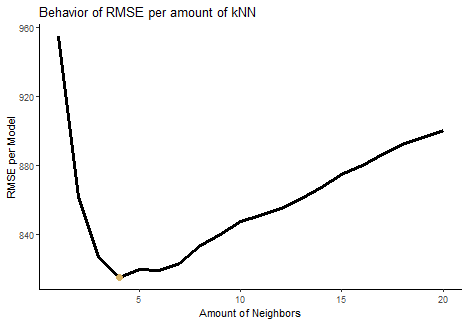
\includegraphics{Diamonds_files/figure-latex/Compute best K-1} \end{center}

\begin{Shaded}
\begin{Highlighting}[]
\CommentTok{\# computing kNN with knnreg from caret package}
\NormalTok{opt\_kNN }\OtherTok{=} \FunctionTok{knnreg}\NormalTok{(}\AttributeTok{x =}\NormalTok{ knn\_train\_norm[, }\SpecialCharTok{{-}}\FunctionTok{c}\NormalTok{(}\DecValTok{1}\NormalTok{)] , }\AttributeTok{y =}\NormalTok{ knn\_train\_norm}\SpecialCharTok{$}\NormalTok{price, }\AttributeTok{k =} \DecValTok{4}\NormalTok{)}

\CommentTok{\# predicting prices of validation set on the validation data}
\NormalTok{opt\_knn\_pred\_y }\OtherTok{=} \FunctionTok{predict}\NormalTok{(}\AttributeTok{object =}\NormalTok{ opt\_kNN, }\AttributeTok{newdata =}\NormalTok{ knn\_valid\_norm[, }\SpecialCharTok{{-}}\FunctionTok{c}\NormalTok{(}\DecValTok{1}\NormalTok{)])}

\CommentTok{\# scaling back (Y*mu + sigma)}
\NormalTok{opt\_knn\_rescaled\_prices }\OtherTok{=}\NormalTok{ std\_price }\SpecialCharTok{*}\NormalTok{ opt\_knn\_pred\_y }\SpecialCharTok{+}\NormalTok{ mean\_price}

\CommentTok{\# computing accuracy measures}
\NormalTok{opt\_accuracy }\OtherTok{\textless{}{-}} \FunctionTok{accuracy}\NormalTok{(}\AttributeTok{object =}\NormalTok{ opt\_knn\_rescaled\_prices, }\AttributeTok{x =}\NormalTok{ real\_prices)}
\FunctionTok{kable\_styling}\NormalTok{(}\FunctionTok{kable}\NormalTok{(opt\_accuracy)}\SpecialCharTok{\%\textgreater{}\%} \FunctionTok{kable\_classic}\NormalTok{(), }\AttributeTok{full\_width =} \ConstantTok{TRUE}\NormalTok{)}
\end{Highlighting}
\end{Shaded}

\begin{table}
\centering
\begin{tabu} to \linewidth {>{\raggedright}X>{\raggedleft}X>{\raggedleft}X>{\raggedleft}X>{\raggedleft}X>{\raggedleft}X}
\hline
  & ME & RMSE & MAE & MPE & MAPE\\
\hline
Test set & 40.86142 & 814.594 & 431.2913 & -2.45264 & 12.13511\\
\hline
\end{tabu}
\end{table}

\hypertarget{regression-tree}{%
\subsection{Regression Tree}\label{regression-tree}}

\hypertarget{partitioning}{%
\subsubsection{Partitioning}\label{partitioning}}

\begin{Shaded}
\begin{Highlighting}[]
\CommentTok{\#Rename data specifically for regression trees}
\NormalTok{diamonds\_tree }\OtherTok{\textless{}{-}}\NormalTok{ diamonds}

\CommentTok{\# Creating data tables Train, Valid and Test using the indexes for the regression tree section}
\NormalTok{Train\_rg }\OtherTok{\textless{}{-}}\NormalTok{ diamonds[train.index, ]}
\NormalTok{Valid\_rg }\OtherTok{\textless{}{-}}\NormalTok{ diamonds[valid.index, ]}
\end{Highlighting}
\end{Shaded}

\hypertarget{regression-tree-1}{%
\subsubsection{Regression Tree}\label{regression-tree-1}}

\begin{Shaded}
\begin{Highlighting}[]
\CommentTok{\# Use rpart() to run tree on continuous response }
\NormalTok{RegressTree }\OtherTok{\textless{}{-}} \FunctionTok{rpart}\NormalTok{(price }\SpecialCharTok{\textasciitilde{}}\NormalTok{ ., }
              \AttributeTok{data =}\NormalTok{ Train\_rg, }
              \AttributeTok{method =} \StringTok{"anova"}\NormalTok{) }

\CommentTok{\# Generates a cost complexity parameter table that provides the complexity parameter value}
\CommentTok{\#summary(RegressTree)}

\CommentTok{\# Plots a regression tree}
\FunctionTok{fancyRpartPlot}\NormalTok{(RegressTree, }\AttributeTok{caption =} \ConstantTok{NULL}\NormalTok{, }\AttributeTok{main =} \StringTok{"Regression Tree"}\NormalTok{, }\AttributeTok{palettes =} \StringTok{"YlGnBu"}\NormalTok{, }\AttributeTok{digits =} \SpecialCharTok{{-}}\DecValTok{3}\NormalTok{)}
\end{Highlighting}
\end{Shaded}

\begin{center}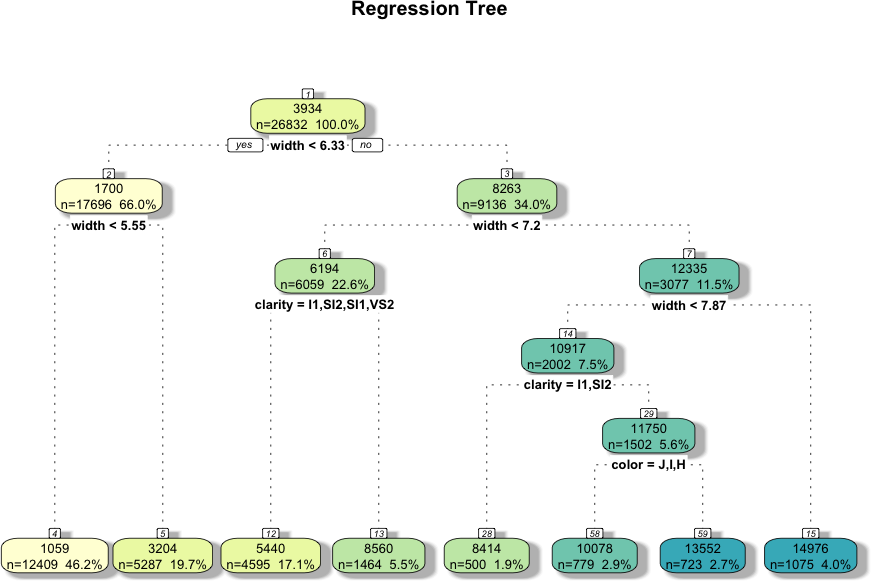
\includegraphics{Diamonds_files/figure-latex/Default Regression Tree-1} \end{center}

\begin{Shaded}
\begin{Highlighting}[]
\CommentTok{\# Count number of leaves }
\FunctionTok{length}\NormalTok{(RegressTree}\SpecialCharTok{$}\NormalTok{frame}\SpecialCharTok{$}\NormalTok{var[RegressTree}\SpecialCharTok{$}\NormalTok{frame}\SpecialCharTok{$}\NormalTok{var }\SpecialCharTok{==} \StringTok{"\textless{}leaf\textgreater{}"}\NormalTok{]) }
\end{Highlighting}
\end{Shaded}

\begin{verbatim}
## [1] 8
\end{verbatim}

\begin{Shaded}
\begin{Highlighting}[]
\CommentTok{\# kable and kable\_styling as before}
\CommentTok{\# We multiply by 100, divide by the sum and round the percentages to 2 decimals}
\FunctionTok{kable\_styling}\NormalTok{(}\FunctionTok{kable}\NormalTok{(}\FunctionTok{round}\NormalTok{(}\DecValTok{100}\SpecialCharTok{*}\NormalTok{RegressTree}\SpecialCharTok{$}\NormalTok{variable.importance }\SpecialCharTok{/} \FunctionTok{sum}\NormalTok{(RegressTree}\SpecialCharTok{$}\NormalTok{variable.importance), }\DecValTok{2}\NormalTok{), }\AttributeTok{col.names =} \StringTok{"Importance \%"}\NormalTok{), }\AttributeTok{full\_width =} \ConstantTok{TRUE}\NormalTok{) }\SpecialCharTok{\%\textgreater{}\%} \FunctionTok{kable\_classic}\NormalTok{() }
\end{Highlighting}
\end{Shaded}

\begin{tabu} to \linewidth {>{\raggedright}X>{\raggedleft}X}
\hline
  & Importance \%\\
\hline
width & 25.50\\
\hline
length & 24.30\\
\hline
carat & 23.90\\
\hline
depth & 22.57\\
\hline
clarity & 2.53\\
\hline
color & 1.08\\
\hline
depth\_ratio & 0.09\\
\hline
table & 0.02\\
\hline
cut & 0.01\\
\hline
\end{tabu}

\begin{Shaded}
\begin{Highlighting}[]
\CommentTok{\# Predict errors using accuracy() }
\NormalTok{tree\_aa1 }\OtherTok{\textless{}{-}}\NormalTok{ forecast}\SpecialCharTok{::}\FunctionTok{accuracy}\NormalTok{(}\FunctionTok{predict}\NormalTok{(RegressTree, Valid\_rg), Valid\_rg}\SpecialCharTok{$}\NormalTok{price)}

\FunctionTok{kable\_styling}\NormalTok{(}\FunctionTok{kable}\NormalTok{(tree\_aa1)}\SpecialCharTok{\%\textgreater{}\%} \FunctionTok{kable\_classic}\NormalTok{(), }\AttributeTok{full\_width =} \ConstantTok{TRUE}\NormalTok{)}
\end{Highlighting}
\end{Shaded}

\begin{table}
\centering
\begin{tabu} to \linewidth {>{\raggedright}X>{\raggedleft}X>{\raggedleft}X>{\raggedleft}X>{\raggedleft}X>{\raggedleft}X}
\hline
  & ME & RMSE & MAE & MPE & MAPE\\
\hline
Test set & 6.097627 & 1267.154 & 846.9286 & -14.54158 & 33.08388\\
\hline
\end{tabu}
\end{table}

\begin{Shaded}
\begin{Highlighting}[]
\CommentTok{\# Predict the diamond price with validation}
\NormalTok{pred\_Diamond\_test }\OtherTok{\textless{}{-}} \FunctionTok{predict}\NormalTok{(RegressTree, }\AttributeTok{newdata =}\NormalTok{ Valid\_rg)}

\CommentTok{\# Display first 14 observations}
\FunctionTok{head}\NormalTok{(pred\_Diamond\_test,}\DecValTok{14}\NormalTok{)}
\end{Highlighting}
\end{Shaded}

\begin{verbatim}
##        1        2        3        4        5        6        7        8        9       10       11       12
## 5440.419 1059.257 1059.257 8560.343 1059.257 1059.257 3203.633 8414.236 3203.633 1059.257 5440.419 1059.257
##       13       14
## 1059.257 5440.419
\end{verbatim}

\hypertarget{exlcusion-regression-tree}{%
\subsubsection{`Exlcusion' Regression
Tree}\label{exlcusion-regression-tree}}

\begin{Shaded}
\begin{Highlighting}[]
\NormalTok{RegressTree2 }\OtherTok{\textless{}{-}} \FunctionTok{rpart}\NormalTok{(price }\SpecialCharTok{\textasciitilde{}}\NormalTok{ length}\SpecialCharTok{+}\NormalTok{width}\SpecialCharTok{+}\NormalTok{depth}\SpecialCharTok{+}\NormalTok{carat}\SpecialCharTok{+}\NormalTok{cut}\SpecialCharTok{+}\NormalTok{color}\SpecialCharTok{+}\NormalTok{clarity, }
              \AttributeTok{data =}\NormalTok{ Train\_rg, }
              \AttributeTok{method =} \StringTok{"anova"}\NormalTok{) }

\CommentTok{\# Generates a cost complexity parameter table that provides the complexity parameter value}
\CommentTok{\#summary(RegressTree2)}

\CommentTok{\# Plots a regression tree}
\FunctionTok{fancyRpartPlot}\NormalTok{(RegressTree2, }\AttributeTok{caption =} \ConstantTok{NULL}\NormalTok{, }\AttributeTok{main =} \StringTok{"Exclusion Regression Tree"}\NormalTok{, }\AttributeTok{palettes =} \StringTok{"YlGnBu"}\NormalTok{, }\AttributeTok{digits =} \SpecialCharTok{{-}}\DecValTok{3}\NormalTok{)}
\end{Highlighting}
\end{Shaded}

\begin{center}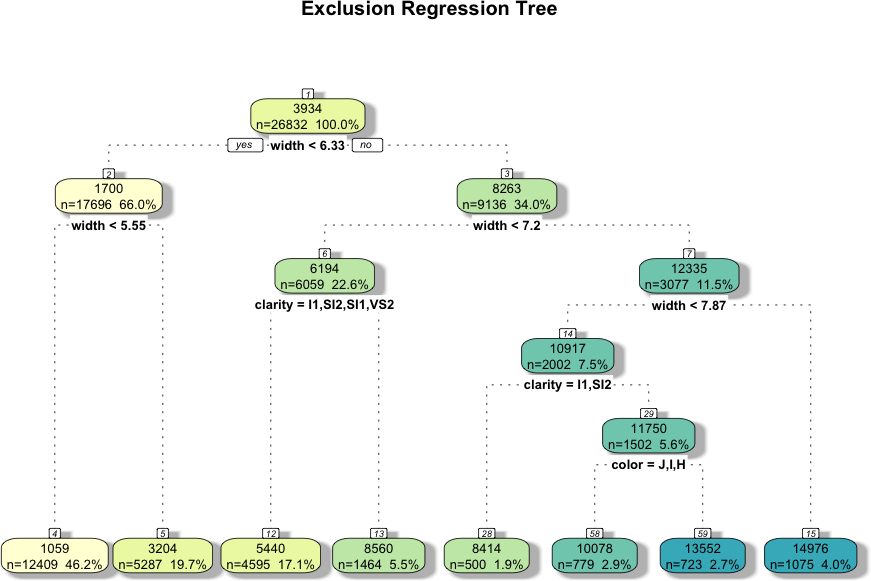
\includegraphics{Diamonds_files/figure-latex/Default Regression Tree Minus Variables-1} \end{center}

\begin{Shaded}
\begin{Highlighting}[]
\CommentTok{\# kable and kable\_styling as before}
\CommentTok{\# We multiply by 100, divide by the sum and round the percentages to 2 decimals}
\FunctionTok{kable\_styling}\NormalTok{(}\FunctionTok{kable}\NormalTok{(}\FunctionTok{round}\NormalTok{(}\DecValTok{100}\SpecialCharTok{*}\NormalTok{RegressTree2}\SpecialCharTok{$}\NormalTok{variable.importance }\SpecialCharTok{/} \FunctionTok{sum}\NormalTok{(RegressTree2}\SpecialCharTok{$}\NormalTok{variable.importance), }\DecValTok{2}\NormalTok{), }\AttributeTok{col.names =} \StringTok{"Importance \%"}\NormalTok{), }\AttributeTok{full\_width =} \ConstantTok{TRUE}\NormalTok{) }\SpecialCharTok{\%\textgreater{}\%} \FunctionTok{kable\_classic}\NormalTok{() }
\end{Highlighting}
\end{Shaded}

\begin{tabu} to \linewidth {>{\raggedright}X>{\raggedleft}X}
\hline
  & Importance \%\\
\hline
width & 25.51\\
\hline
length & 24.31\\
\hline
carat & 23.91\\
\hline
depth & 22.58\\
\hline
clarity & 2.55\\
\hline
color & 1.08\\
\hline
cut & 0.05\\
\hline
\end{tabu}

\begin{Shaded}
\begin{Highlighting}[]
\CommentTok{\# Predict errors using accuracy() }
\NormalTok{tree\_aa2 }\OtherTok{\textless{}{-}}\NormalTok{ forecast}\SpecialCharTok{::}\FunctionTok{accuracy}\NormalTok{(}\FunctionTok{predict}\NormalTok{(RegressTree2, Valid\_rg), Valid\_rg}\SpecialCharTok{$}\NormalTok{price)}

\FunctionTok{kable\_styling}\NormalTok{(}\FunctionTok{kable}\NormalTok{(tree\_aa2)}\SpecialCharTok{\%\textgreater{}\%} \FunctionTok{kable\_classic}\NormalTok{(), }\AttributeTok{full\_width =} \ConstantTok{TRUE}\NormalTok{)}
\end{Highlighting}
\end{Shaded}

\begin{table}
\centering
\begin{tabu} to \linewidth {>{\raggedright}X>{\raggedleft}X>{\raggedleft}X>{\raggedleft}X>{\raggedleft}X>{\raggedleft}X}
\hline
  & ME & RMSE & MAE & MPE & MAPE\\
\hline
Test set & 6.097627 & 1267.154 & 846.9286 & -14.54158 & 33.08388\\
\hline
\end{tabu}
\end{table}

\begin{Shaded}
\begin{Highlighting}[]
\CommentTok{\# Predict the diamond price with validation}
\NormalTok{pred\_Diamond\_test }\OtherTok{\textless{}{-}} \FunctionTok{predict}\NormalTok{(RegressTree, }\AttributeTok{newdata =}\NormalTok{ Valid\_rg)}

\CommentTok{\# Display first 14 observations}
\FunctionTok{head}\NormalTok{(pred\_Diamond\_test,}\DecValTok{14}\NormalTok{)}
\end{Highlighting}
\end{Shaded}

\begin{verbatim}
##        1        2        3        4        5        6        7        8        9       10       11       12
## 5440.419 1059.257 1059.257 8560.343 1059.257 1059.257 3203.633 8414.236 3203.633 1059.257 5440.419 1059.257
##       13       14
## 1059.257 5440.419
\end{verbatim}

\begin{Shaded}
\begin{Highlighting}[]
\CommentTok{\#Get the lowest CP value from CP table}
\NormalTok{min.xerror }\OtherTok{\textless{}{-}}\NormalTok{ RegressTree2}\SpecialCharTok{$}\NormalTok{cptable[}\FunctionTok{which.min}\NormalTok{(RegressTree2}\SpecialCharTok{$}\NormalTok{cptable[,}\StringTok{"xerror"}\NormalTok{]),}\StringTok{"CP"}\NormalTok{]}

\NormalTok{min.xerror}
\end{Highlighting}
\end{Shaded}

\begin{verbatim}
## [1] 0.01
\end{verbatim}

\begin{Shaded}
\begin{Highlighting}[]
\CommentTok{\#Plot the optimal Cp value}
\FunctionTok{plotcp}\NormalTok{(RegressTree2)}
\end{Highlighting}
\end{Shaded}

\begin{center}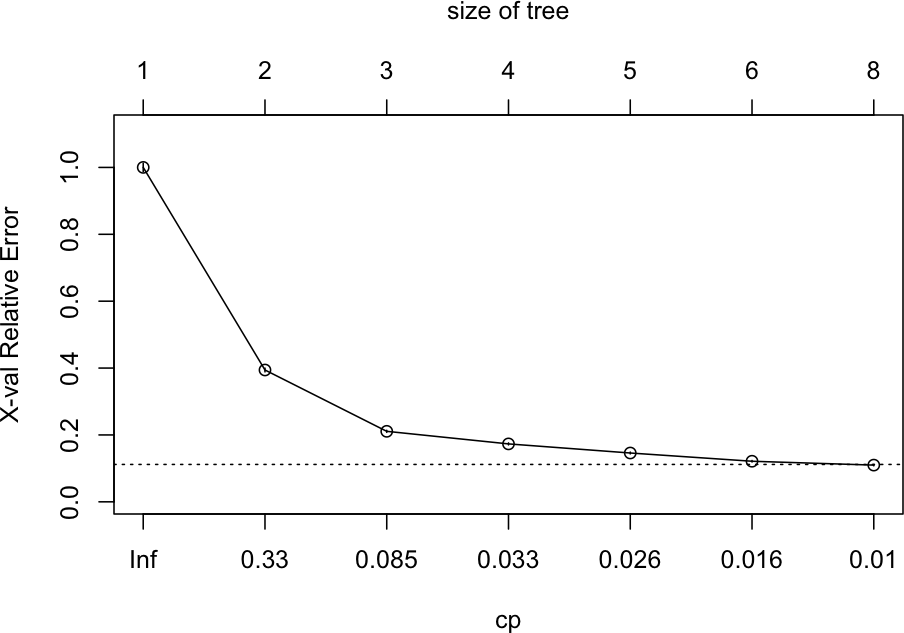
\includegraphics{Diamonds_files/figure-latex/Plot Cp-1} \end{center}

\hypertarget{pruned-regression-tree}{%
\subsubsection{Pruned Regression Tree}\label{pruned-regression-tree}}

\begin{Shaded}
\begin{Highlighting}[]
\NormalTok{RegressTree\_pruned }\OtherTok{\textless{}{-}} \FunctionTok{prune}\NormalTok{(RegressTree2, }\AttributeTok{cp =}\NormalTok{ min.xerror) }

\CommentTok{\# Draw the prune tree}
\FunctionTok{fancyRpartPlot}\NormalTok{(RegressTree\_pruned, }\AttributeTok{caption =} \ConstantTok{NULL}\NormalTok{, }\AttributeTok{main =} \StringTok{"\textquotesingle{}Pruned\textquotesingle{} Regression Tree"}\NormalTok{, }\AttributeTok{palettes =} \StringTok{"YlGnBu"}\NormalTok{, }\AttributeTok{digits =} \SpecialCharTok{{-}}\DecValTok{3}\NormalTok{)}
\end{Highlighting}
\end{Shaded}

\begin{center}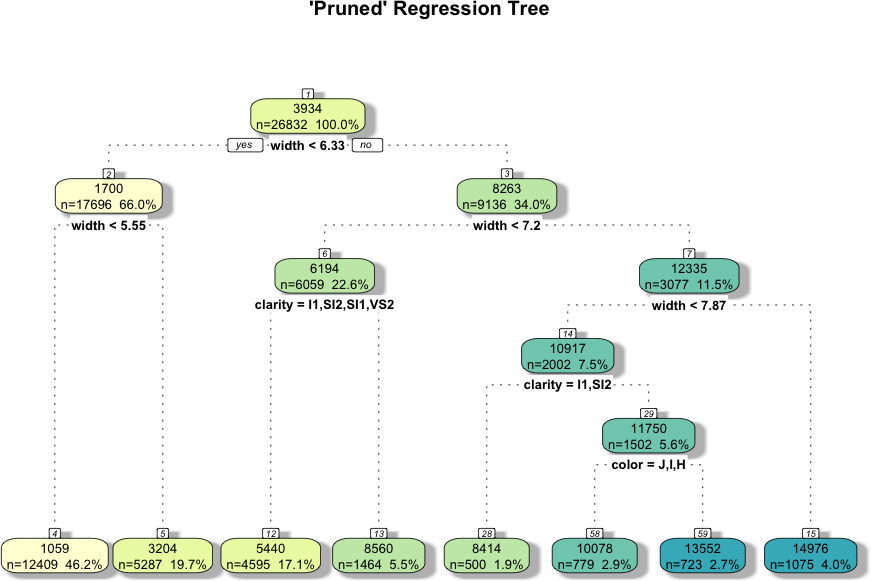
\includegraphics{Diamonds_files/figure-latex/Pruned Regression Tree Minus Variables-1} \end{center}

\begin{Shaded}
\begin{Highlighting}[]
\CommentTok{\# Predict errors using accuracy() }
\NormalTok{tree\_aa3 }\OtherTok{\textless{}{-}}\NormalTok{ forecast}\SpecialCharTok{::}\FunctionTok{accuracy}\NormalTok{(}\FunctionTok{predict}\NormalTok{(RegressTree\_pruned, Valid\_rg), Valid\_rg}\SpecialCharTok{$}\NormalTok{price)}

\FunctionTok{kable\_styling}\NormalTok{(}\FunctionTok{kable}\NormalTok{(tree\_aa3)}\SpecialCharTok{\%\textgreater{}\%} \FunctionTok{kable\_classic}\NormalTok{(), }\AttributeTok{full\_width =} \ConstantTok{TRUE}\NormalTok{) }
\end{Highlighting}
\end{Shaded}

\begin{table}
\centering
\begin{tabu} to \linewidth {>{\raggedright}X>{\raggedleft}X>{\raggedleft}X>{\raggedleft}X>{\raggedleft}X>{\raggedleft}X}
\hline
  & ME & RMSE & MAE & MPE & MAPE\\
\hline
Test set & 6.097627 & 1267.154 & 846.9286 & -14.54158 & 33.08388\\
\hline
\end{tabu}
\end{table}

\hypertarget{boosted-tree}{%
\subsubsection{Boosted Tree}\label{boosted-tree}}

\begin{Shaded}
\begin{Highlighting}[]
\CommentTok{\# Boosted tree}
\FunctionTok{set.seed}\NormalTok{(}\DecValTok{111}\NormalTok{)}
\NormalTok{tree\_boost10 }\OtherTok{\textless{}{-}} \FunctionTok{gbm}\NormalTok{(price }\SpecialCharTok{\textasciitilde{}}\NormalTok{., }\AttributeTok{data =}\NormalTok{ Train\_rg, }\AttributeTok{distribution =} \StringTok{"gaussian"}\NormalTok{, }\AttributeTok{n.trees =} \DecValTok{10}\NormalTok{, }\AttributeTok{interaction.depth =} \DecValTok{6}\NormalTok{, }\AttributeTok{shrinkage =} \FloatTok{0.01}\NormalTok{)}

\CommentTok{\# Interaction Depth specifies the maximum depth of each tree( i.e. highest level of variable interactions allowed while training the model). Default is 1.}
\CommentTok{\# Shrinkage is considered as the learning rate. It is used for reducing, or shrinking, the impact of each additional fitted base{-}learner (tree).  It reduces the size of incremental steps and thus penalizes the importance of each consecutive iteration. Default is 0.1}
\CommentTok{\#n.trees: Integer specifying the total number of trees to fit. This is equivalent to the number of iterations and the number of basis functions in the additive expansion. Default is 100.}


\NormalTok{tree\_boost10}
\end{Highlighting}
\end{Shaded}

\begin{verbatim}
## gbm(formula = price ~ ., distribution = "gaussian", data = Train_rg,
##     n.trees = 10, interaction.depth = 6, shrinkage = 0.01)
## A gradient boosted model with gaussian loss function.
## 10 iterations were performed.
## There were 9 predictors of which 5 had non-zero influence.
\end{verbatim}

\begin{Shaded}
\begin{Highlighting}[]
\NormalTok{vip}\SpecialCharTok{::}\FunctionTok{vip}\NormalTok{(tree\_boost10, }\AttributeTok{aesthetics =} \FunctionTok{list}\NormalTok{(}\AttributeTok{fill =} \StringTok{"\#D8B365"}\NormalTok{)) }\SpecialCharTok{+}
  \FunctionTok{ggtitle}\NormalTok{(}\StringTok{"Boosted Tree Variable Importance"}\NormalTok{) }\SpecialCharTok{+} \CommentTok{\# Title name}
  \FunctionTok{xlab}\NormalTok{(}\StringTok{"Variable"}\NormalTok{) }\SpecialCharTok{+} \CommentTok{\# Label names}
  \FunctionTok{theme\_classic}\NormalTok{() }\CommentTok{\# A classic theme, with x and y axis lines and no grid lines}
\end{Highlighting}
\end{Shaded}

\begin{center}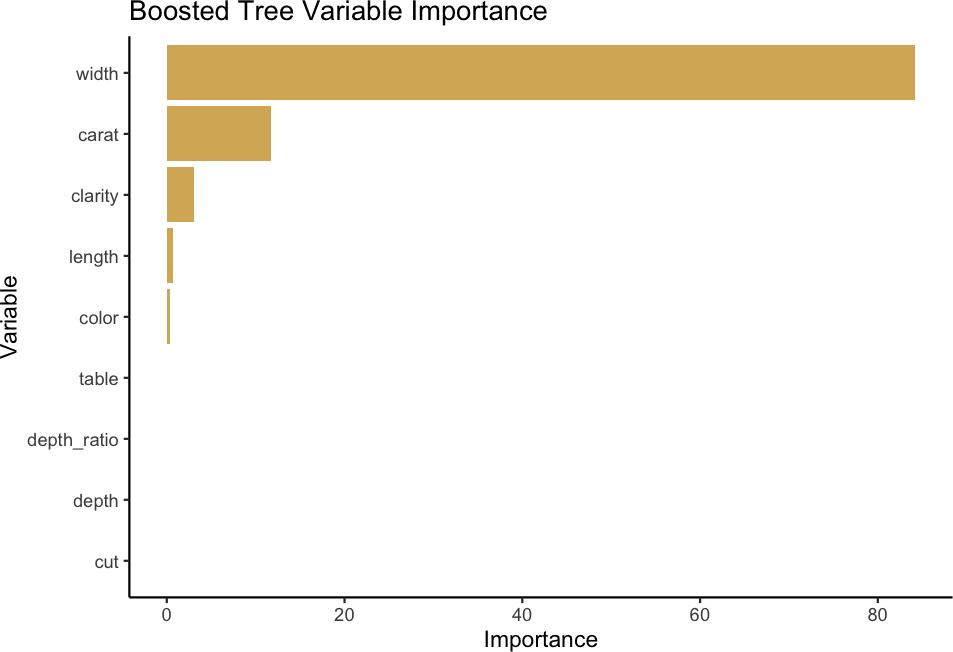
\includegraphics{Diamonds_files/figure-latex/Boosted Tree 10-1} \end{center}

\begin{Shaded}
\begin{Highlighting}[]
\CommentTok{\# Predict errors using accuracy()}
\NormalTok{tree\_aa4 }\OtherTok{\textless{}{-}}\NormalTok{ forecast}\SpecialCharTok{::}\FunctionTok{accuracy}\NormalTok{(}\FunctionTok{predict}\NormalTok{(tree\_boost10, Valid\_rg), Valid\_rg}\SpecialCharTok{$}\NormalTok{price)}

\FunctionTok{kable\_styling}\NormalTok{(}\FunctionTok{kable}\NormalTok{(tree\_aa4)}\SpecialCharTok{\%\textgreater{}\%} \FunctionTok{kable\_classic}\NormalTok{(), }\AttributeTok{full\_width =} \ConstantTok{TRUE}\NormalTok{) }
\end{Highlighting}
\end{Shaded}

\begin{table}
\centering
\begin{tabu} to \linewidth {>{\raggedright}X>{\raggedleft}X>{\raggedleft}X>{\raggedleft}X>{\raggedleft}X>{\raggedleft}X}
\hline
  & ME & RMSE & MAE & MPE & MAPE\\
\hline
Test set & -3.898022 & 3660.422 & 2765.963 & -144.4894 & 171.6511\\
\hline
\end{tabu}
\end{table}

\begin{Shaded}
\begin{Highlighting}[]
\CommentTok{\# Boosted tree}
\FunctionTok{set.seed}\NormalTok{(}\DecValTok{111}\NormalTok{)}
\NormalTok{tree\_boost30 }\OtherTok{\textless{}{-}} \FunctionTok{gbm}\NormalTok{(price }\SpecialCharTok{\textasciitilde{}}\NormalTok{., }\AttributeTok{data =}\NormalTok{ Train\_rg, }\AttributeTok{distribution =} \StringTok{"gaussian"}\NormalTok{, }\AttributeTok{n.trees =} \DecValTok{30}\NormalTok{)}

\NormalTok{vip}\SpecialCharTok{::}\FunctionTok{vip}\NormalTok{(tree\_boost30, }\AttributeTok{aesthetics =} \FunctionTok{list}\NormalTok{(}\AttributeTok{fill =} \StringTok{"\#D8B365"}\NormalTok{)) }\SpecialCharTok{+}
  \FunctionTok{ggtitle}\NormalTok{(}\StringTok{"Boosted Tree Variable Importance"}\NormalTok{) }\SpecialCharTok{+} \CommentTok{\# Title name}
  \FunctionTok{xlab}\NormalTok{(}\StringTok{"Variable"}\NormalTok{) }\SpecialCharTok{+} \CommentTok{\# Label names}
  \FunctionTok{theme\_classic}\NormalTok{() }\CommentTok{\# A classic theme, with x and y axis lines and no grid lines}
\end{Highlighting}
\end{Shaded}

\begin{center}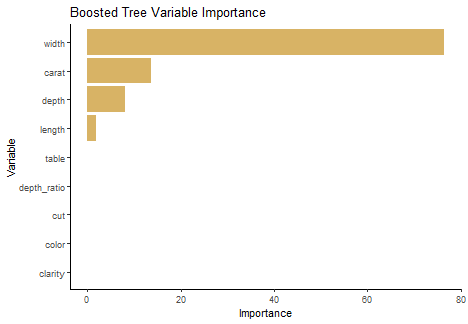
\includegraphics{Diamonds_files/figure-latex/Boosted Tree 30-1} \end{center}

\begin{Shaded}
\begin{Highlighting}[]
\NormalTok{tree\_boost30}
\end{Highlighting}
\end{Shaded}

\begin{verbatim}
## gbm(formula = price ~ ., distribution = "gaussian", data = Train_rg,
##     n.trees = 30)
## A gradient boosted model with gaussian loss function.
## 30 iterations were performed.
## There were 9 predictors of which 4 had non-zero influence.
\end{verbatim}

\begin{Shaded}
\begin{Highlighting}[]
\CommentTok{\# Predict errors using accuracy() }
\NormalTok{tree\_aa5 }\OtherTok{\textless{}{-}}\NormalTok{ forecast}\SpecialCharTok{::}\FunctionTok{accuracy}\NormalTok{(}\FunctionTok{predict}\NormalTok{(tree\_boost30, Train\_rg), Train\_rg}\SpecialCharTok{$}\NormalTok{price)}

\FunctionTok{kable\_styling}\NormalTok{(}\FunctionTok{kable}\NormalTok{(tree\_aa5)}\SpecialCharTok{\%\textgreater{}\%} \FunctionTok{kable\_classic}\NormalTok{(), }\AttributeTok{full\_width =} \ConstantTok{TRUE}\NormalTok{)  }
\end{Highlighting}
\end{Shaded}

\begin{table}
\centering
\begin{tabu} to \linewidth {>{\raggedright}X>{\raggedleft}X>{\raggedleft}X>{\raggedleft}X>{\raggedleft}X>{\raggedleft}X}
\hline
  & ME & RMSE & MAE & MPE & MAPE\\
\hline
Test set & 2.5438 & 1531.521 & 985.6974 & -35.25731 & 46.85606\\
\hline
\end{tabu}
\end{table}

\begin{Shaded}
\begin{Highlighting}[]
\CommentTok{\# Boosted tree}
\FunctionTok{set.seed}\NormalTok{(}\DecValTok{111}\NormalTok{)}
\NormalTok{tree\_boost100 }\OtherTok{\textless{}{-}} \FunctionTok{gbm}\NormalTok{(price }\SpecialCharTok{\textasciitilde{}}\NormalTok{., }\AttributeTok{data =}\NormalTok{ Train\_rg, }\AttributeTok{distribution =} \StringTok{"gaussian"}\NormalTok{, }\AttributeTok{cv.folds =} \DecValTok{3}\NormalTok{)}

\CommentTok{\# cv.folds: Number of cross{-}validation folds to perform. If cv.folds\textgreater{}1 then gbm, in addition to the usual fit, will perform a cross{-}validation, calculate an estimate of generalization error returned in cv.error.}

\NormalTok{vip}\SpecialCharTok{::}\FunctionTok{vip}\NormalTok{(tree\_boost100, }\AttributeTok{aesthetics =} \FunctionTok{list}\NormalTok{(}\AttributeTok{fill =} \StringTok{"\#D8B365"}\NormalTok{)) }\SpecialCharTok{+}
  \FunctionTok{ggtitle}\NormalTok{(}\StringTok{"Boosted Tree Variable Importance"}\NormalTok{) }\SpecialCharTok{+} \CommentTok{\# Title name}
  \FunctionTok{xlab}\NormalTok{(}\StringTok{"Variable"}\NormalTok{) }\SpecialCharTok{+} \CommentTok{\# Label names}
  \FunctionTok{theme\_classic}\NormalTok{() }\CommentTok{\# A classic theme, with x and y axis lines and no grid lines}
\end{Highlighting}
\end{Shaded}

\begin{center}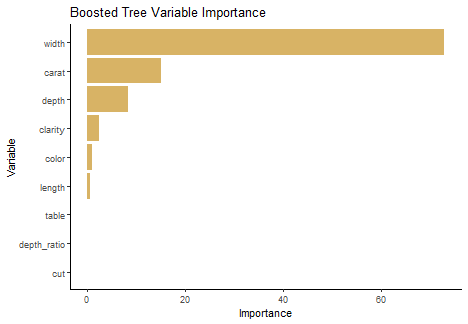
\includegraphics{Diamonds_files/figure-latex/Boosted Tree 100-1} \end{center}

\begin{Shaded}
\begin{Highlighting}[]
\NormalTok{tree\_boost100}
\end{Highlighting}
\end{Shaded}

\begin{verbatim}
## gbm(formula = price ~ ., distribution = "gaussian", data = Train_rg,
##     cv.folds = 3)
## A gradient boosted model with gaussian loss function.
## 100 iterations were performed.
## The best cross-validation iteration was 100.
## There were 9 predictors of which 6 had non-zero influence.
\end{verbatim}

\begin{Shaded}
\begin{Highlighting}[]
\CommentTok{\# Predict errors using accuracy() }
\NormalTok{tree\_aa6 }\OtherTok{\textless{}{-}}\NormalTok{ forecast}\SpecialCharTok{::}\FunctionTok{accuracy}\NormalTok{(}\FunctionTok{predict}\NormalTok{(tree\_boost100, Valid\_rg), Valid\_rg}\SpecialCharTok{$}\NormalTok{price)}

\FunctionTok{kable\_styling}\NormalTok{(}\FunctionTok{kable}\NormalTok{(tree\_aa6)}\SpecialCharTok{\%\textgreater{}\%} \FunctionTok{kable\_classic}\NormalTok{(), }\AttributeTok{full\_width =} \ConstantTok{TRUE}\NormalTok{) }
\end{Highlighting}
\end{Shaded}

\begin{table}
\centering
\begin{tabu} to \linewidth {>{\raggedright}X>{\raggedleft}X>{\raggedleft}X>{\raggedleft}X>{\raggedleft}X>{\raggedleft}X}
\hline
  & ME & RMSE & MAE & MPE & MAPE\\
\hline
Test set & 9.002539 & 1170.295 & 680.2182 & -12.85125 & 26.22023\\
\hline
\end{tabu}
\end{table}

\begin{Shaded}
\begin{Highlighting}[]
\NormalTok{pred\_boost }\OtherTok{\textless{}{-}} \FunctionTok{predict.gbm}\NormalTok{(tree\_boost100, }\AttributeTok{newdata =}\NormalTok{ Valid\_rg)}

\FunctionTok{head}\NormalTok{(pred\_boost, }\DecValTok{14}\NormalTok{)}
\end{Highlighting}
\end{Shaded}

\begin{verbatim}
##  [1] 6112.0846 1582.6043  743.7071 6352.0316 1140.2701 1491.0859 2806.4714 9855.1238 2681.4129 1330.4517
## [11] 7595.4454 1741.6017 1380.0364 6132.5267
\end{verbatim}

\hypertarget{bagging-tree}{%
\subsubsection{Bagging Tree}\label{bagging-tree}}

\begin{Shaded}
\begin{Highlighting}[]
\CommentTok{\# Bagged tree}
\FunctionTok{set.seed}\NormalTok{(}\DecValTok{111}\NormalTok{)}
\NormalTok{tree\_bagging }\OtherTok{\textless{}{-}} \FunctionTok{bagging}\NormalTok{(price }\SpecialCharTok{\textasciitilde{}}\NormalTok{., }\AttributeTok{data =}\NormalTok{ Train\_rg, }\AttributeTok{coob =} \ConstantTok{TRUE}\NormalTok{)}
\NormalTok{tree\_bagging}
\end{Highlighting}
\end{Shaded}

\begin{verbatim}
##
## Bagging regression trees with 25 bootstrap replications
##
## Call: bagging.data.frame(formula = price ~ ., data = Train_rg, coob = TRUE)
##
## Out-of-bag estimate of root mean squared error:  1268.231
\end{verbatim}

\begin{Shaded}
\begin{Highlighting}[]
\NormalTok{ss}\OtherTok{\textless{}{-}}\FunctionTok{varImp}\NormalTok{(tree\_bagging)}

\NormalTok{data}\OtherTok{\textless{}{-}}\FunctionTok{data.table}\NormalTok{(}\AttributeTok{name=}\FunctionTok{row.names}\NormalTok{(ss),}\AttributeTok{value=}\NormalTok{ss}\SpecialCharTok{$}\NormalTok{Overall)}

\NormalTok{data[,}\FunctionTok{ggplot}\NormalTok{(.SD, }\FunctionTok{aes}\NormalTok{(}\AttributeTok{x=}\FunctionTok{reorder}\NormalTok{(name, ss}\SpecialCharTok{$}\NormalTok{Overall), }\AttributeTok{y=}\NormalTok{ss}\SpecialCharTok{$}\NormalTok{Overall)) }\SpecialCharTok{+}
  \FunctionTok{geom\_bar}\NormalTok{(}\AttributeTok{stat =} \StringTok{"identity"}\NormalTok{, }\AttributeTok{fill =} \StringTok{"\#D8B365"}\NormalTok{) }\SpecialCharTok{+}
  \FunctionTok{xlab}\NormalTok{(}\StringTok{"Variable"}\NormalTok{) }\SpecialCharTok{+} \CommentTok{\# Label names + }
  \FunctionTok{ylab}\NormalTok{(}\StringTok{"Importance"}\NormalTok{) }\SpecialCharTok{+} \CommentTok{\# Label names + }
  \FunctionTok{ggtitle}\NormalTok{(}\StringTok{"Bagged Tree Variable Importance"}\NormalTok{) }\SpecialCharTok{+} \CommentTok{\# Title name}
  \FunctionTok{theme\_classic}\NormalTok{() }\SpecialCharTok{+} \CommentTok{\# A classic theme, with x and y axis lines and no grid lines}
  \FunctionTok{coord\_flip}\NormalTok{(),]}
\end{Highlighting}
\end{Shaded}

\begin{center}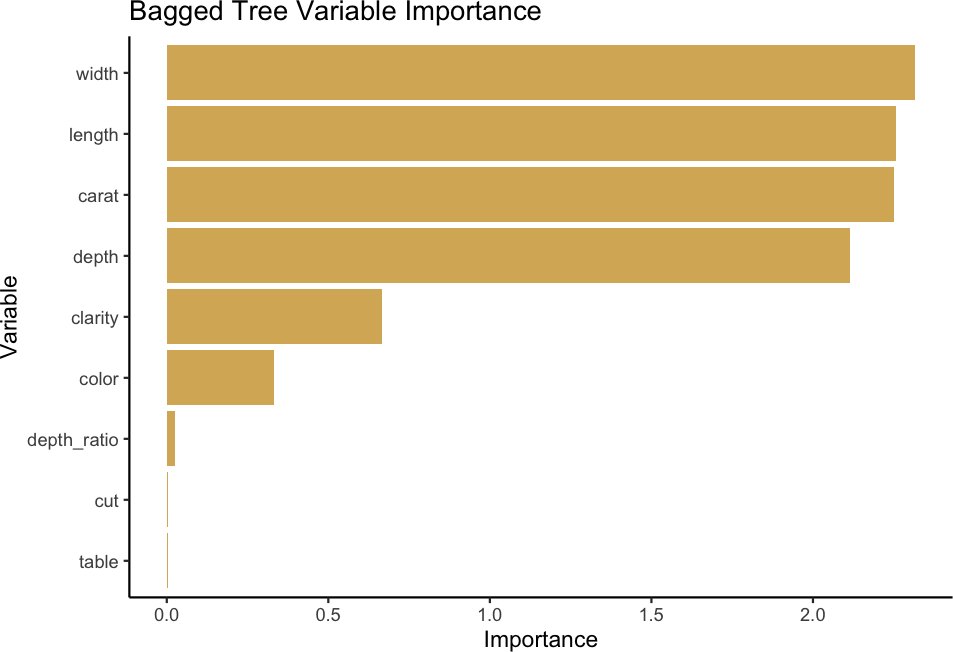
\includegraphics{Diamonds_files/figure-latex/Plot IV Bagging-1} \end{center}

\begin{Shaded}
\begin{Highlighting}[]
\NormalTok{tree\_aa7 }\OtherTok{\textless{}{-}}\NormalTok{ forecast}\SpecialCharTok{::}\FunctionTok{accuracy}\NormalTok{(}\FunctionTok{predict}\NormalTok{(tree\_bagging, Valid\_rg), Valid\_rg}\SpecialCharTok{$}\NormalTok{price)}

\FunctionTok{kable\_styling}\NormalTok{(}\FunctionTok{kable}\NormalTok{(tree\_aa7)}\SpecialCharTok{\%\textgreater{}\%} \FunctionTok{kable\_classic}\NormalTok{(), }\AttributeTok{full\_width =} \ConstantTok{TRUE}\NormalTok{) }
\end{Highlighting}
\end{Shaded}

\begin{table}
\centering
\begin{tabu} to \linewidth {>{\raggedright}X>{\raggedleft}X>{\raggedleft}X>{\raggedleft}X>{\raggedleft}X>{\raggedleft}X}
\hline
  & ME & RMSE & MAE & MPE & MAPE\\
\hline
Test set & 0.9333074 & 1248.769 & 808.9297 & -14.35086 & 31.45019\\
\hline
\end{tabu}
\end{table}

\begin{Shaded}
\begin{Highlighting}[]
\NormalTok{pred\_bagged }\OtherTok{\textless{}{-}} \FunctionTok{predict}\NormalTok{(tree\_bagging, }\AttributeTok{newdata =}\NormalTok{ Valid\_rg)}

\FunctionTok{head}\NormalTok{(pred\_bagged,}\DecValTok{14}\NormalTok{)}
\end{Highlighting}
\end{Shaded}

\begin{verbatim}
##  [1]  5396.881  1104.498  1046.993  8084.493  1104.498  1104.498  3123.791 10274.884  3123.791  1046.993
## [11]  6052.800  1104.498  1046.993  5953.609
\end{verbatim}

\hypertarget{randomforest}{%
\subsubsection{RandomForest}\label{randomforest}}

\begin{Shaded}
\begin{Highlighting}[]
\FunctionTok{options}\NormalTok{(}\AttributeTok{scipen =} \DecValTok{9999}\NormalTok{)}

\CommentTok{\# Create randomForest}
\FunctionTok{set.seed}\NormalTok{(}\DecValTok{111}\NormalTok{)}
\NormalTok{rdf\_model }\OtherTok{\textless{}{-}} \FunctionTok{randomForest}\NormalTok{(price}\SpecialCharTok{\textasciitilde{}}\NormalTok{ ., }\AttributeTok{ntree=} \DecValTok{60}\NormalTok{, }\AttributeTok{data =}\NormalTok{ Train\_rg)}
\NormalTok{rdf\_model}
\end{Highlighting}
\end{Shaded}

\begin{verbatim}
##
## Call:
##  randomForest(formula = price ~ ., data = Train_rg, ntree = 60)
##                Type of random forest: regression
##                      Number of trees: 60
## No. of variables tried at each split: 3
##
##           Mean of squared residuals: 335950
##                     % Var explained: 97.89
\end{verbatim}

\begin{Shaded}
\begin{Highlighting}[]
\FunctionTok{plot}\NormalTok{(rdf\_model,}
         \AttributeTok{main =} \StringTok{"Number of Optimal Trees"}\NormalTok{)}
\end{Highlighting}
\end{Shaded}

\begin{center}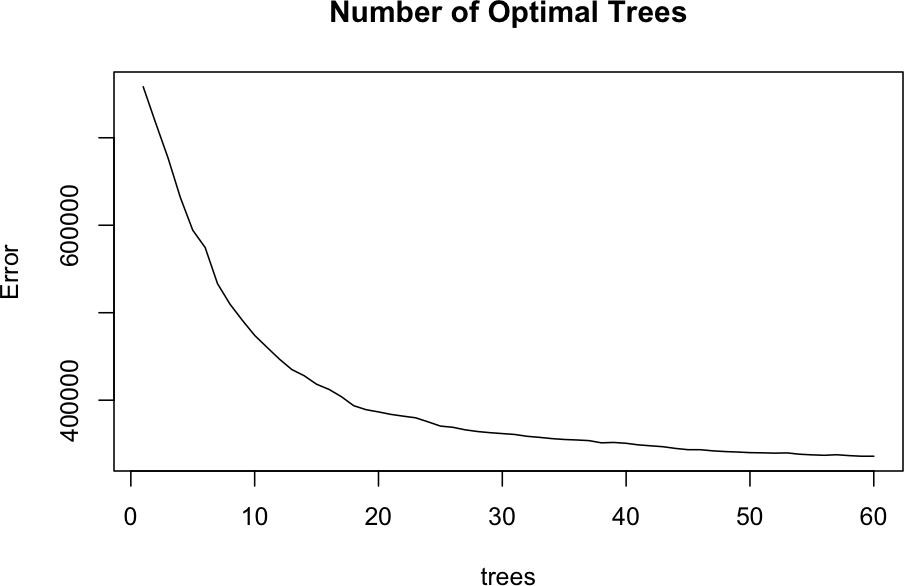
\includegraphics{Diamonds_files/figure-latex/randomForest-1} \end{center}

\begin{Shaded}
\begin{Highlighting}[]
\CommentTok{\# Number of trees with lowest MSE}
\CommentTok{\# Compared with 80 and 100 trees, the trade{-}off with both of those were small so we stuck with 60 trees}
\FunctionTok{which.min}\NormalTok{(rdf\_model}\SpecialCharTok{$}\NormalTok{mse)}
\end{Highlighting}
\end{Shaded}

\begin{verbatim}
## [1] 59
\end{verbatim}

\begin{Shaded}
\begin{Highlighting}[]
\FunctionTok{options}\NormalTok{(}\AttributeTok{scipen =} \DecValTok{9999}\NormalTok{)}

\CommentTok{\# Create variable importance chart}
\NormalTok{vip}\SpecialCharTok{::}\FunctionTok{vip}\NormalTok{(rdf\_model, }\AttributeTok{aesthetics =} \FunctionTok{list}\NormalTok{(}\AttributeTok{fill =} \StringTok{"\#D8B365"}\NormalTok{)) }\SpecialCharTok{+}
  \FunctionTok{ggtitle}\NormalTok{(}\StringTok{"RandomTree Variable Importance"}\NormalTok{) }\SpecialCharTok{+} \CommentTok{\# Title name}
  \FunctionTok{xlab}\NormalTok{(}\StringTok{"Variable"}\NormalTok{) }\SpecialCharTok{+} \CommentTok{\# Label names}
  \FunctionTok{theme\_classic}\NormalTok{() }\CommentTok{\# A classic theme, with x and y axis lines and no grid lines}
\end{Highlighting}
\end{Shaded}

\begin{center}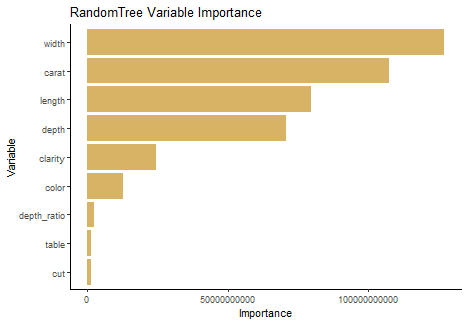
\includegraphics{Diamonds_files/figure-latex/RF Variable Importance-1} \end{center}

\begin{Shaded}
\begin{Highlighting}[]
\NormalTok{tree\_aa8 }\OtherTok{\textless{}{-}}\NormalTok{ forecast}\SpecialCharTok{::}\FunctionTok{accuracy}\NormalTok{(}\FunctionTok{predict}\NormalTok{(rdf\_model, Valid\_rg), Valid\_rg}\SpecialCharTok{$}\NormalTok{price)}

\FunctionTok{kable\_styling}\NormalTok{(}\FunctionTok{kable}\NormalTok{(tree\_aa8)}\SpecialCharTok{\%\textgreater{}\%} \FunctionTok{kable\_classic}\NormalTok{(), }\AttributeTok{full\_width =} \ConstantTok{TRUE}\NormalTok{) }
\end{Highlighting}
\end{Shaded}

\begin{table}
\centering
\begin{tabu} to \linewidth {>{\raggedright}X>{\raggedleft}X>{\raggedleft}X>{\raggedleft}X>{\raggedleft}X>{\raggedleft}X}
\hline
  & ME & RMSE & MAE & MPE & MAPE\\
\hline
Test set & 2.969775 & 577.63 & 289.5139 & -1.402886 & 7.235286\\
\hline
\end{tabu}
\end{table}

\begin{Shaded}
\begin{Highlighting}[]
\NormalTok{pred\_random }\OtherTok{\textless{}{-}} \FunctionTok{predict}\NormalTok{(rdf\_model, }\AttributeTok{newdata =}\NormalTok{ Valid\_rg)}

\FunctionTok{head}\NormalTok{(pred\_random,}\DecValTok{14}\NormalTok{)}
\end{Highlighting}
\end{Shaded}

\begin{verbatim}
##         1         2         3         4         5         6         7         8         9        10        11
## 5012.2100 1782.6600  591.9428 9185.5925 1319.5133 1344.4381 2423.8250 8620.2650 2562.5817  936.9519 9243.9557
##        12        13        14
## 1788.5992 1172.3436 7014.9981
\end{verbatim}

\hypertarget{create-regression-tree-summary-table}{%
\subsubsection{Create Regression Tree Summary
Table}\label{create-regression-tree-summary-table}}

\begin{Shaded}
\begin{Highlighting}[]
\NormalTok{Tree\_res }\OtherTok{\textless{}{-}} \FunctionTok{data.frame}\NormalTok{(}\StringTok{"Model\_Tree"} \OtherTok{=} \FunctionTok{c}\NormalTok{(}\StringTok{"Reg. Tree"}\NormalTok{,}
                                 \StringTok{"Exclus. RT"}\NormalTok{,}
                                 \StringTok{"Pruned RT"}\NormalTok{,}
                                 \StringTok{"Boost10"}\NormalTok{,}
                                 \StringTok{"Boost30"}\NormalTok{,}
                                 \StringTok{"Boost100"}\NormalTok{,}
                                 \StringTok{"Bagging"}\NormalTok{,}
                                 \StringTok{"RndmFrst"}\NormalTok{),}
                     \StringTok{"ME"} \OtherTok{=} \StringTok{""}\NormalTok{,}
                     \StringTok{"RMSE"} \OtherTok{=} \StringTok{""}\NormalTok{,}
                     \StringTok{"MAE"}\OtherTok{=} \StringTok{""}\NormalTok{,}
                     \StringTok{"MPE"} \OtherTok{=} \StringTok{""}\NormalTok{,}
                     \StringTok{"MAPE"} \OtherTok{=} \StringTok{""}\NormalTok{)}

\FunctionTok{rownames}\NormalTok{(Tree\_res) }\OtherTok{\textless{}{-}}\NormalTok{ Tree\_res}\SpecialCharTok{$}\NormalTok{Model\_Tree}
\NormalTok{Tree\_res}\SpecialCharTok{$}\NormalTok{Model\_Tree }\OtherTok{=} \ConstantTok{NULL}

\ControlFlowTok{for}\NormalTok{ (i }\ControlFlowTok{in} \DecValTok{1}\SpecialCharTok{:}\DecValTok{8}\NormalTok{) \{}
\NormalTok{  Tree\_res[i,]}\OtherTok{=} \FunctionTok{round}\NormalTok{(}\FunctionTok{get}\NormalTok{(}\FunctionTok{paste}\NormalTok{(}\StringTok{"tree\_aa"}\NormalTok{, i, }\AttributeTok{sep =}\StringTok{""}\NormalTok{)),}\DecValTok{2}\NormalTok{)}
\NormalTok{\}}

\FunctionTok{kable\_styling}\NormalTok{(}\FunctionTok{kable}\NormalTok{(Tree\_res)}\SpecialCharTok{\%\textgreater{}\%} \FunctionTok{kable\_classic}\NormalTok{(), }\AttributeTok{full\_width =} \ConstantTok{TRUE}\NormalTok{)}
\end{Highlighting}
\end{Shaded}

\begin{table}
\centering
\begin{tabu} to \linewidth {>{\raggedright}X>{\raggedright}X>{\raggedright}X>{\raggedright}X>{\raggedright}X>{\raggedright}X}
\hline
  & ME & RMSE & MAE & MPE & MAPE\\
\hline
Reg. Tree & 6.1 & 1267.15 & 846.93 & -14.54 & 33.08\\
\hline
Exclus. RT & 6.1 & 1267.15 & 846.93 & -14.54 & 33.08\\
\hline
Pruned RT & 6.1 & 1267.15 & 846.93 & -14.54 & 33.08\\
\hline
Boost10 & -3.9 & 3660.42 & 2765.96 & -144.49 & 171.65\\
\hline
Boost30 & 2.54 & 1531.52 & 985.7 & -35.26 & 46.86\\
\hline
Boost100 & 9 & 1170.3 & 680.22 & -12.85 & 26.22\\
\hline
Bagging & 0.93 & 1248.77 & 808.93 & -14.35 & 31.45\\
\hline
RndmFrst & 2.97 & 577.63 & 289.51 & -1.4 & 7.24\\
\hline
\end{tabu}
\end{table}

\begin{Shaded}
\begin{Highlighting}[]
\NormalTok{RGRMSEplotdata }\OtherTok{\textless{}{-}} \FunctionTok{t}\NormalTok{(Tree\_res}\SpecialCharTok{$}\NormalTok{RMSE)}
\FunctionTok{colnames}\NormalTok{(RGRMSEplotdata) }\OtherTok{\textless{}{-}} \FunctionTok{t}\NormalTok{(}\FunctionTok{sort}\NormalTok{(}\FunctionTok{rownames}\NormalTok{(Tree\_res),}\AttributeTok{decreasing =} \ConstantTok{TRUE}\NormalTok{))}
\NormalTok{RGRMSEplotdata}
\end{Highlighting}
\end{Shaded}

\begin{verbatim}
##      RndmFrst  Reg. Tree Pruned RT Exclus. RT Boost30   Boost100 Boost10   Bagging
## [1,] "1267.15" "1267.15" "1267.15" "3660.42"  "1531.52" "1170.3" "1248.77" "577.63"
\end{verbatim}

\begin{Shaded}
\begin{Highlighting}[]
\FunctionTok{barplot}\NormalTok{(RGRMSEplotdata, }\AttributeTok{col =} \StringTok{"\#D8B365"}\NormalTok{,}\AttributeTok{border =} \StringTok{"\#D8B365"}\NormalTok{ ,}
         \AttributeTok{main =} \StringTok{"Regression Tree Comparison"}\NormalTok{, }\AttributeTok{ylab =} \StringTok{"RMSE"}\NormalTok{, }\AttributeTok{las =} \DecValTok{3}\NormalTok{, }\AttributeTok{ylim=}\FunctionTok{c}\NormalTok{(}\DecValTok{0}\NormalTok{,}\DecValTok{4000}\NormalTok{))}
\end{Highlighting}
\end{Shaded}

\begin{center}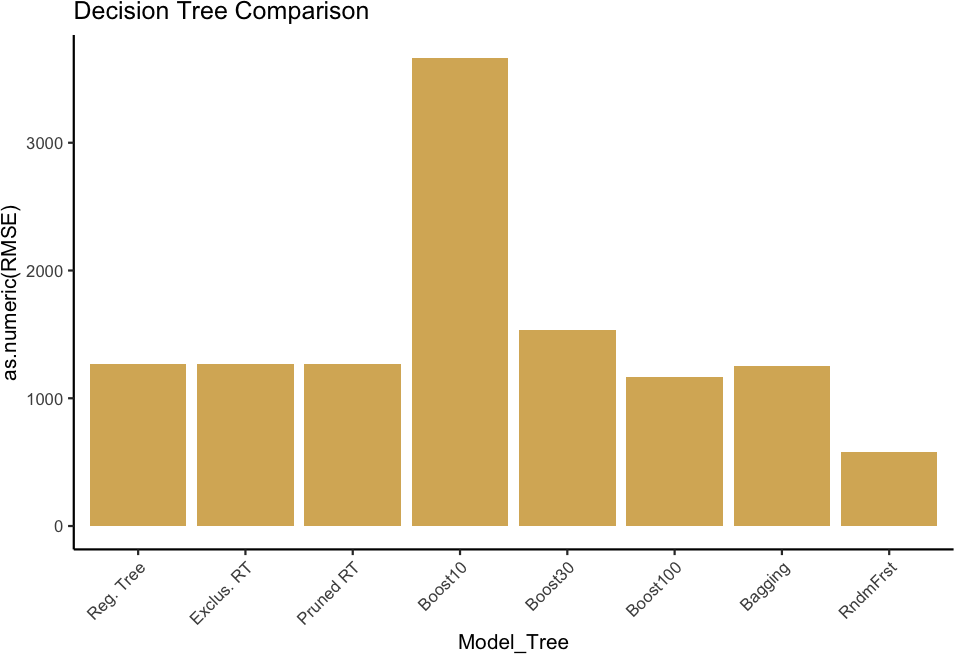
\includegraphics{Diamonds_files/figure-latex/RegTree Summary-1} \end{center}

\hypertarget{neuralnetworks}{%
\subsection{NeuralNetworks}\label{neuralnetworks}}

\hypertarget{data-preprocessing}{%
\subsubsection{Data preprocessing}\label{data-preprocessing}}

\begin{Shaded}
\begin{Highlighting}[]
\CommentTok{\#create dummy columns }
\NormalTok{diamonds\_dummies }\OtherTok{\textless{}{-}} \FunctionTok{dummy\_cols}\NormalTok{(diamonds, }\AttributeTok{select\_columns =} \FunctionTok{c}\NormalTok{(}\StringTok{"cut"}\NormalTok{, }\StringTok{"color"}\NormalTok{, }\StringTok{"clarity"}\NormalTok{))}
\NormalTok{diamonds\_dummies }\OtherTok{\textless{}{-}}\NormalTok{ diamonds\_dummies[,}\SpecialCharTok{{-}}\FunctionTok{c}\NormalTok{(}\DecValTok{2}\SpecialCharTok{:}\DecValTok{4}\NormalTok{)]}

\CommentTok{\#rename column to avoid issues with Neural net function}
\FunctionTok{colnames}\NormalTok{(diamonds\_dummies)[}\DecValTok{10}\NormalTok{] }\OtherTok{=} \StringTok{"cut\_Very\_Good"}
\end{Highlighting}
\end{Shaded}

\hypertarget{partitioning-1}{%
\subsubsection{Partitioning}\label{partitioning-1}}

\begin{Shaded}
\begin{Highlighting}[]
\NormalTok{Train\_nn }\OtherTok{\textless{}{-}}\NormalTok{ diamonds\_dummies[train.index,]}
\NormalTok{Valid\_nn }\OtherTok{\textless{}{-}}\NormalTok{ diamonds\_dummies[valid.index,]}
\end{Highlighting}
\end{Shaded}

\hypertarget{normalizing-data}{%
\subsubsection{Normalizing Data}\label{normalizing-data}}

\begin{Shaded}
\begin{Highlighting}[]
\CommentTok{\# use preProcess() to normalize non{-}categorical variables}
\NormalTok{norm\_values }\OtherTok{\textless{}{-}} \FunctionTok{preProcess}\NormalTok{(Train\_nn[}\DecValTok{1}\SpecialCharTok{:}\DecValTok{7}\NormalTok{], }\AttributeTok{method=} \FunctionTok{c}\NormalTok{(}\StringTok{"range"}\NormalTok{))}

\NormalTok{Train\_nn\_norm }\OtherTok{\textless{}{-}} \FunctionTok{predict}\NormalTok{(norm\_values, Train\_nn)}
\NormalTok{Valid\_nn\_norm }\OtherTok{\textless{}{-}} \FunctionTok{predict}\NormalTok{(norm\_values, Valid\_nn)}
\end{Highlighting}
\end{Shaded}

\hypertarget{model-1-layers-1-nodes-1}{%
\subsubsection{Model 1 (Layers = 1, Nodes =
1)}\label{model-1-layers-1-nodes-1}}

\begin{itemize}
\tightlist
\item
  Creating Model 1
\end{itemize}

\begin{Shaded}
\begin{Highlighting}[]
\CommentTok{\#create data sets to train and validate the model}
\CommentTok{\#train}
\NormalTok{x\_train }\OtherTok{\textless{}{-}} \FunctionTok{c}\NormalTok{(}\FunctionTok{t}\NormalTok{(Train\_nn\_norm[, }\SpecialCharTok{{-}}\FunctionTok{c}\NormalTok{(}\DecValTok{1}\NormalTok{)]))}
\NormalTok{x\_train }\OtherTok{\textless{}{-}} \FunctionTok{as.array}\NormalTok{(x\_train,}
                    \FunctionTok{dim}\NormalTok{(}\FunctionTok{t}\NormalTok{(Train\_nn\_norm[, }\SpecialCharTok{{-}}\FunctionTok{c}\NormalTok{(}\DecValTok{1}\NormalTok{)])),}
                    \AttributeTok{dimnames =} \FunctionTok{list}\NormalTok{(}\FunctionTok{rownames}\NormalTok{(x\_train), }\FunctionTok{colnames}\NormalTok{(x\_train)))}
\NormalTok{x\_train }\OtherTok{\textless{}{-}} \FunctionTok{as\_tensor}\NormalTok{(x\_train, }\AttributeTok{shape =} \FunctionTok{dim}\NormalTok{(Train\_nn\_norm[, }\SpecialCharTok{{-}}\FunctionTok{c}\NormalTok{(}\DecValTok{1}\NormalTok{)]))}
\NormalTok{y\_train }\OtherTok{\textless{}{-}} \FunctionTok{as\_tensor}\NormalTok{(Train\_nn\_norm}\SpecialCharTok{$}\NormalTok{price)}

\CommentTok{\#validation}
\NormalTok{x\_valid }\OtherTok{\textless{}{-}} \FunctionTok{c}\NormalTok{(}\FunctionTok{t}\NormalTok{(Valid\_nn\_norm[, }\SpecialCharTok{{-}}\FunctionTok{c}\NormalTok{(}\DecValTok{1}\NormalTok{)]))}
\NormalTok{x\_valid }\OtherTok{\textless{}{-}} \FunctionTok{as.array}\NormalTok{(x\_valid,}
                    \FunctionTok{dim}\NormalTok{(}\FunctionTok{t}\NormalTok{(Valid\_nn\_norm[, }\SpecialCharTok{{-}}\FunctionTok{c}\NormalTok{(}\DecValTok{1}\NormalTok{)])),}
                    \AttributeTok{dimnames =} \FunctionTok{list}\NormalTok{(}\FunctionTok{rownames}\NormalTok{(x\_valid), }\FunctionTok{colnames}\NormalTok{(x\_valid)))}
\NormalTok{x\_valid }\OtherTok{\textless{}{-}} \FunctionTok{as\_tensor}\NormalTok{(x\_valid, }\AttributeTok{shape =} \FunctionTok{dim}\NormalTok{(Valid\_nn\_norm[, }\SpecialCharTok{{-}}\FunctionTok{c}\NormalTok{(}\DecValTok{1}\NormalTok{)]))}
\NormalTok{y\_valid }\OtherTok{\textless{}{-}} \FunctionTok{as\_tensor}\NormalTok{(Valid\_nn\_norm}\SpecialCharTok{$}\NormalTok{price)}

\CommentTok{\#create model}
\FunctionTok{rm}\NormalTok{(model\_1\_1) }\CommentTok{\#to prevent retraining of existing model}
\NormalTok{tf}\SpecialCharTok{$}\NormalTok{random}\SpecialCharTok{$}\FunctionTok{set\_seed}\NormalTok{(}\DecValTok{111}\NormalTok{)}
\NormalTok{model\_1\_1 }\OtherTok{\textless{}{-}} \FunctionTok{keras\_model\_sequential}\NormalTok{(}\AttributeTok{input\_shape =} \FunctionTok{ncol}\NormalTok{(x\_train)) }\SpecialCharTok{\%\textgreater{}\%}
  \FunctionTok{layer\_dense}\NormalTok{(}\DecValTok{1}\NormalTok{, }\AttributeTok{activation =} \StringTok{"sigmoid"}\NormalTok{, }\AttributeTok{name =} \StringTok{"HiddenLayer"}\NormalTok{) }\SpecialCharTok{\%\textgreater{}\%}  \CommentTok{\# 1st hidden layer (26 nodes)}
  \FunctionTok{layer\_dense}\NormalTok{(}\DecValTok{1}\NormalTok{, }\AttributeTok{activation =} \StringTok{"sigmoid"}\NormalTok{, }\AttributeTok{name =} \StringTok{"outputLayer"}\NormalTok{)     }\CommentTok{\# output layer (1 node)}


\CommentTok{\#compile the model to be trained            }
\NormalTok{model\_1\_1 }\SpecialCharTok{\%\textgreater{}\%} \FunctionTok{compile}\NormalTok{(}
  \AttributeTok{optimizer =} \FunctionTok{optimizer\_adam}\NormalTok{(),}
  \AttributeTok{loss =} \FunctionTok{loss\_mean\_squared\_error}\NormalTok{(),}
  \AttributeTok{metric =} \FunctionTok{metric\_root\_mean\_squared\_error}\NormalTok{()}
\NormalTok{  )}

\CommentTok{\#train the model and find the lowest rmse}
\NormalTok{history }\OtherTok{\textless{}{-}}\NormalTok{ model\_1\_1 }\SpecialCharTok{\%\textgreater{}\%} \FunctionTok{fit}\NormalTok{(}
    \AttributeTok{x =}\NormalTok{ x\_train,}
    \AttributeTok{y =}\NormalTok{ y\_train,}
    \AttributeTok{validation\_data =} \FunctionTok{c}\NormalTok{(x\_valid, y\_valid),}
    \AttributeTok{verbose =} \ConstantTok{FALSE}
\NormalTok{    )}
\end{Highlighting}
\end{Shaded}

\begin{itemize}
\tightlist
\item
  Measuring Error Model 1
\end{itemize}

\begin{Shaded}
\begin{Highlighting}[]
\CommentTok{\# prediction values of validation set}
\NormalTok{y\_valid\_pred }\OtherTok{\textless{}{-}} \FunctionTok{predict}\NormalTok{(model\_1\_1, x\_valid)}

\CommentTok{\# fetching a and b from standardization for scaling back price}
\NormalTok{a }\OtherTok{\textless{}{-}}\NormalTok{ norm\_values}\SpecialCharTok{$}\NormalTok{ranges[}\DecValTok{1}\NormalTok{,}\DecValTok{1}\NormalTok{]}
\NormalTok{b }\OtherTok{\textless{}{-}}\NormalTok{ norm\_values}\SpecialCharTok{$}\NormalTok{ranges[}\DecValTok{2}\NormalTok{,}\DecValTok{1}\NormalTok{]}

\NormalTok{valRescale }\OtherTok{\textless{}{-}} \ControlFlowTok{function}\NormalTok{ (x) \{ }
\NormalTok{  value }\OtherTok{\textless{}{-}}\NormalTok{ (x }\SpecialCharTok{*}\NormalTok{ (b}\SpecialCharTok{{-}}\NormalTok{a) }\SpecialCharTok{+}\NormalTok{ a)}
  \FunctionTok{return}\NormalTok{(value)}
\NormalTok{\}}

\CommentTok{\# scaling back price predictions}
\NormalTok{y\_valid\_pred }\OtherTok{\textless{}{-}} \FunctionTok{valRescale}\NormalTok{(y\_valid\_pred)}

\CommentTok{\# we have to change the class of y\_valid\_pred}
\FunctionTok{class}\NormalTok{(y\_valid\_pred)}
\end{Highlighting}
\end{Shaded}

\begin{verbatim}
## [1] "matrix" "array"
\end{verbatim}

\begin{Shaded}
\begin{Highlighting}[]
\NormalTok{y\_valid\_pred }\OtherTok{\textless{}{-}} \FunctionTok{as.numeric}\NormalTok{(y\_valid\_pred)}
\FunctionTok{class}\NormalTok{(y\_valid\_pred)}
\end{Highlighting}
\end{Shaded}

\begin{verbatim}
## [1] "numeric"
\end{verbatim}

\begin{Shaded}
\begin{Highlighting}[]
\CommentTok{\# taking real values of validation set from original data (which wasn\textquotesingle{}t standardized!)}
\NormalTok{y\_valid\_real }\OtherTok{\textless{}{-}}\NormalTok{ diamonds[valid.index, price]}

\CommentTok{\# copmuting accuracy measures of validation set}
\NormalTok{acc\_1 }\OtherTok{\textless{}{-}} \FunctionTok{accuracy}\NormalTok{(}\AttributeTok{object =}\NormalTok{ y\_valid\_pred, }\AttributeTok{x =}\NormalTok{ y\_valid\_real)}

\FunctionTok{kable\_styling}\NormalTok{(}\FunctionTok{kable}\NormalTok{(acc\_1)}\SpecialCharTok{\%\textgreater{}\%} \FunctionTok{kable\_classic}\NormalTok{(), }\AttributeTok{full\_width =} \ConstantTok{TRUE}\NormalTok{)}
\end{Highlighting}
\end{Shaded}

\begin{table}
\centering
\begin{tabu} to \linewidth {>{\raggedright}X>{\raggedleft}X>{\raggedleft}X>{\raggedleft}X>{\raggedleft}X>{\raggedleft}X}
\hline
  & ME & RMSE & MAE & MPE & MAPE\\
\hline
Test set & -6.616364 & 3982.992 & 3025.611 & -157.4749 & 187.2922\\
\hline
\end{tabu}
\end{table}

\hypertarget{model-2-layers-1-nodes-26}{%
\subsubsection{Model 2 (Layers = 1, Nodes =
26)}\label{model-2-layers-1-nodes-26}}

\begin{itemize}
\tightlist
\item
  Creating Model 2
\end{itemize}

\begin{Shaded}
\begin{Highlighting}[]
\CommentTok{\#create model}
\FunctionTok{rm}\NormalTok{(model\_1\_26) }\CommentTok{\#to prevent retraining of existing model}
\NormalTok{tf}\SpecialCharTok{$}\NormalTok{random}\SpecialCharTok{$}\FunctionTok{set\_seed}\NormalTok{(}\DecValTok{111}\NormalTok{)}
\NormalTok{model\_1\_26 }\OtherTok{\textless{}{-}} \FunctionTok{keras\_model\_sequential}\NormalTok{(}\AttributeTok{input\_shape =} \FunctionTok{ncol}\NormalTok{(x\_train)) }\SpecialCharTok{\%\textgreater{}\%}
  \FunctionTok{layer\_dense}\NormalTok{(}\DecValTok{26}\NormalTok{, }\AttributeTok{activation =} \StringTok{"sigmoid"}\NormalTok{, }\AttributeTok{name =} \StringTok{"HiddenLayer"}\NormalTok{) }\SpecialCharTok{\%\textgreater{}\%}  \CommentTok{\# 1st hidden layer (26 nodes)}
  \FunctionTok{layer\_dense}\NormalTok{(}\DecValTok{1}\NormalTok{, }\AttributeTok{activation =} \StringTok{"sigmoid"}\NormalTok{, }\AttributeTok{name =} \StringTok{"outputLayer"}\NormalTok{)     }\CommentTok{\# output layer (1 node)}


\CommentTok{\#compile the model to be trained            }
\NormalTok{model\_1\_26 }\SpecialCharTok{\%\textgreater{}\%} \FunctionTok{compile}\NormalTok{(}
  \AttributeTok{optimizer =} \FunctionTok{optimizer\_adam}\NormalTok{(),}
  \AttributeTok{loss =} \FunctionTok{loss\_mean\_squared\_error}\NormalTok{(),}
  \AttributeTok{metric =} \FunctionTok{metric\_root\_mean\_squared\_error}\NormalTok{()}
\NormalTok{  )}

\CommentTok{\#train the model and find the lowest rmse}
\NormalTok{history }\OtherTok{\textless{}{-}}\NormalTok{ model\_1\_26 }\SpecialCharTok{\%\textgreater{}\%} \FunctionTok{fit}\NormalTok{(}
    \AttributeTok{x =}\NormalTok{ x\_train,}
    \AttributeTok{y =}\NormalTok{ y\_train,}
    \AttributeTok{validation\_data =} \FunctionTok{c}\NormalTok{(x\_valid, y\_valid),}
    \AttributeTok{verbose =} \ConstantTok{FALSE}
\NormalTok{    )}
\end{Highlighting}
\end{Shaded}

\begin{itemize}
\tightlist
\item
  Measuring Error Model 2
\end{itemize}

\begin{Shaded}
\begin{Highlighting}[]
\CommentTok{\# prediction values of validation set}
\NormalTok{y\_valid\_pred\_1\_26 }\OtherTok{\textless{}{-}} \FunctionTok{predict}\NormalTok{(model\_1\_26, x\_valid)}

\CommentTok{\# scaling back price predictions}
\NormalTok{y\_valid\_pred\_1\_26 }\OtherTok{\textless{}{-}} \FunctionTok{valRescale}\NormalTok{(y\_valid\_pred\_1\_26)}

\CommentTok{\# we have to change the class of y\_valid\_pred}
\NormalTok{y\_valid\_pred\_1\_26 }\OtherTok{\textless{}{-}} \FunctionTok{as.numeric}\NormalTok{(y\_valid\_pred\_1\_26)}

\CommentTok{\# computing accuracy measures of validation set}
\NormalTok{acc\_2 }\OtherTok{\textless{}{-}} \FunctionTok{accuracy}\NormalTok{(}\AttributeTok{object =}\NormalTok{ y\_valid\_pred\_1\_26, }\AttributeTok{x =}\NormalTok{ y\_valid\_real)}

\FunctionTok{kable\_styling}\NormalTok{(}\FunctionTok{kable}\NormalTok{(acc\_2)}\SpecialCharTok{\%\textgreater{}\%} \FunctionTok{kable\_classic}\NormalTok{(), }\AttributeTok{full\_width =} \ConstantTok{TRUE}\NormalTok{)}
\end{Highlighting}
\end{Shaded}

\begin{table}
\centering
\begin{tabu} to \linewidth {>{\raggedright}X>{\raggedleft}X>{\raggedleft}X>{\raggedleft}X>{\raggedleft}X>{\raggedleft}X}
\hline
  & ME & RMSE & MAE & MPE & MAPE\\
\hline
Test set & -83.27564 & 745.1569 & 450.941 & -11.36538 & 17.91012\\
\hline
\end{tabu}
\end{table}

\hypertarget{model-3-layers-1-nodes-13}{%
\subsubsection{Model 3 (Layers = 1, Nodes =
13)}\label{model-3-layers-1-nodes-13}}

\begin{itemize}
\tightlist
\item
  Creating Model 3
\end{itemize}

\begin{Shaded}
\begin{Highlighting}[]
\CommentTok{\#create model}
\FunctionTok{rm}\NormalTok{(model\_1\_13) }\CommentTok{\#to prevent retraining of existing model}
\NormalTok{tf}\SpecialCharTok{$}\NormalTok{random}\SpecialCharTok{$}\FunctionTok{set\_seed}\NormalTok{(}\DecValTok{111}\NormalTok{)}
\NormalTok{model\_1\_13 }\OtherTok{\textless{}{-}} \FunctionTok{keras\_model\_sequential}\NormalTok{(}\AttributeTok{input\_shape =} \FunctionTok{ncol}\NormalTok{(x\_train)) }\SpecialCharTok{\%\textgreater{}\%}
  \FunctionTok{layer\_dense}\NormalTok{(}\DecValTok{13}\NormalTok{, }\AttributeTok{activation =} \StringTok{"sigmoid"}\NormalTok{, }\AttributeTok{name =} \StringTok{"HiddenLayer"}\NormalTok{) }\SpecialCharTok{\%\textgreater{}\%}  \CommentTok{\# 1st hidden layer (26 nodes)}
  \FunctionTok{layer\_dense}\NormalTok{(}\DecValTok{1}\NormalTok{, }\AttributeTok{activation =} \StringTok{"sigmoid"}\NormalTok{, }\AttributeTok{name =} \StringTok{"outputLayer"}\NormalTok{)     }\CommentTok{\# output layer (1 node)}


\CommentTok{\#compile the model to be trained            }
\NormalTok{model\_1\_13 }\SpecialCharTok{\%\textgreater{}\%} \FunctionTok{compile}\NormalTok{(}
  \AttributeTok{optimizer =} \FunctionTok{optimizer\_adam}\NormalTok{(),}
  \AttributeTok{loss =} \FunctionTok{loss\_mean\_squared\_error}\NormalTok{(),}
  \AttributeTok{metric =} \FunctionTok{metric\_root\_mean\_squared\_error}\NormalTok{()}
\NormalTok{  )}

\CommentTok{\#train the model and find the lowest rmse}
\NormalTok{history }\OtherTok{\textless{}{-}}\NormalTok{ model\_1\_13 }\SpecialCharTok{\%\textgreater{}\%} \FunctionTok{fit}\NormalTok{(}
    \AttributeTok{x =}\NormalTok{ x\_train,}
    \AttributeTok{y =}\NormalTok{ y\_train,}
    \AttributeTok{validation\_data =} \FunctionTok{c}\NormalTok{(x\_valid, y\_valid),}
    \AttributeTok{verbose =} \ConstantTok{FALSE}
\NormalTok{    )}
\end{Highlighting}
\end{Shaded}

\begin{itemize}
\tightlist
\item
  Measuring Error Model 3
\end{itemize}

\begin{Shaded}
\begin{Highlighting}[]
\CommentTok{\# prediction values of validation set}
\NormalTok{y\_valid\_pred\_1\_13 }\OtherTok{\textless{}{-}} \FunctionTok{predict}\NormalTok{(model\_1\_13, x\_valid)}

\CommentTok{\# scaling back price predictions}
\NormalTok{y\_valid\_pred\_1\_13 }\OtherTok{\textless{}{-}} \FunctionTok{valRescale}\NormalTok{(y\_valid\_pred\_1\_13)}

\CommentTok{\# we have to change the class of y\_valid\_pred}
\NormalTok{y\_valid\_pred\_1\_13 }\OtherTok{\textless{}{-}} \FunctionTok{as.numeric}\NormalTok{(y\_valid\_pred\_1\_13)}

\CommentTok{\# copmuting accuracy measures of validation set}
\NormalTok{acc\_3 }\OtherTok{\textless{}{-}} \FunctionTok{accuracy}\NormalTok{(}\AttributeTok{object =}\NormalTok{ y\_valid\_pred\_1\_13, }\AttributeTok{x =}\NormalTok{ y\_valid\_real)}

\FunctionTok{kable\_styling}\NormalTok{(}\FunctionTok{kable}\NormalTok{(acc\_3)}\SpecialCharTok{\%\textgreater{}\%} \FunctionTok{kable\_classic}\NormalTok{(), }\AttributeTok{full\_width =} \ConstantTok{TRUE}\NormalTok{)}
\end{Highlighting}
\end{Shaded}

\begin{table}
\centering
\begin{tabu} to \linewidth {>{\raggedright}X>{\raggedleft}X>{\raggedleft}X>{\raggedleft}X>{\raggedleft}X>{\raggedleft}X}
\hline
  & ME & RMSE & MAE & MPE & MAPE\\
\hline
Test set & -86.71198 & 744.0357 & 454.3788 & -12.8878 & 19.21285\\
\hline
\end{tabu}
\end{table}

\hypertarget{model-4-layers-2-nodes-26}{%
\subsubsection{Model 4 (Layers = 2, Nodes =
26)}\label{model-4-layers-2-nodes-26}}

\begin{itemize}
\tightlist
\item
  Creating Model 4
\end{itemize}

\begin{Shaded}
\begin{Highlighting}[]
\CommentTok{\#create model}
\FunctionTok{rm}\NormalTok{(model\_2\_26) }\CommentTok{\#to prevent retraining of existing model}
\NormalTok{tf}\SpecialCharTok{$}\NormalTok{random}\SpecialCharTok{$}\FunctionTok{set\_seed}\NormalTok{(}\DecValTok{111}\NormalTok{)}
\NormalTok{model\_2\_26 }\OtherTok{\textless{}{-}} \FunctionTok{keras\_model\_sequential}\NormalTok{(}\AttributeTok{input\_shape =} \FunctionTok{ncol}\NormalTok{(x\_train)) }\SpecialCharTok{\%\textgreater{}\%}
  \FunctionTok{layer\_dense}\NormalTok{(}\DecValTok{26}\NormalTok{, }\AttributeTok{activation =} \StringTok{"sigmoid"}\NormalTok{, }\AttributeTok{name =} \StringTok{"HiddenLayer"}\NormalTok{) }\SpecialCharTok{\%\textgreater{}\%}  \CommentTok{\# 1st hidden layer (26 nodes)}
  \FunctionTok{layer\_dense}\NormalTok{(}\DecValTok{26}\NormalTok{, }\AttributeTok{activation =} \StringTok{"sigmoid"}\NormalTok{, }\AttributeTok{name =} \StringTok{"HiddenLayer2"}\NormalTok{) }\SpecialCharTok{\%\textgreater{}\%}  \CommentTok{\# 2nd hidden layer (26 nodes)}
  \FunctionTok{layer\_dense}\NormalTok{(}\DecValTok{13}\NormalTok{, }\AttributeTok{activation =} \StringTok{"sigmoid"}\NormalTok{, }\AttributeTok{name =} \StringTok{"HiddenLayer3"}\NormalTok{) }\SpecialCharTok{\%\textgreater{}\%}  \CommentTok{\# 3rd hidden layer (26 nodes)}
  \FunctionTok{layer\_dense}\NormalTok{(}\DecValTok{1}\NormalTok{, }\AttributeTok{activation =} \StringTok{"sigmoid"}\NormalTok{, }\AttributeTok{name =} \StringTok{"outputLayer"}\NormalTok{)     }\CommentTok{\# output layer (1 node)}


\CommentTok{\#compile the model to be trained            }
\NormalTok{model\_2\_26 }\SpecialCharTok{\%\textgreater{}\%} \FunctionTok{compile}\NormalTok{(}
  \AttributeTok{optimizer =} \FunctionTok{optimizer\_adam}\NormalTok{(),}
  \AttributeTok{loss =} \FunctionTok{loss\_mean\_squared\_error}\NormalTok{(),}
  \AttributeTok{metric =} \FunctionTok{metric\_root\_mean\_squared\_error}\NormalTok{()}
\NormalTok{  )}

\CommentTok{\#train the model and find the lowest rmse}
\NormalTok{history }\OtherTok{\textless{}{-}}\NormalTok{ model\_2\_26 }\SpecialCharTok{\%\textgreater{}\%} \FunctionTok{fit}\NormalTok{(}
    \AttributeTok{x =}\NormalTok{ x\_train,}
    \AttributeTok{y =}\NormalTok{ y\_train,}
    \AttributeTok{validation\_data =} \FunctionTok{c}\NormalTok{(x\_valid, y\_valid),}
    \AttributeTok{verbose =} \ConstantTok{FALSE}
\NormalTok{    )}
\end{Highlighting}
\end{Shaded}

\begin{itemize}
\tightlist
\item
  Measuring Error Model 4
\end{itemize}

\begin{Shaded}
\begin{Highlighting}[]
\CommentTok{\# prediction values of validation set}
\NormalTok{y\_valid\_pred\_2\_26 }\OtherTok{\textless{}{-}} \FunctionTok{predict}\NormalTok{(model\_2\_26, x\_valid)}

\CommentTok{\# scaling back price predictions}
\NormalTok{y\_valid\_pred\_2\_26 }\OtherTok{\textless{}{-}} \FunctionTok{valRescale}\NormalTok{(y\_valid\_pred\_2\_26)}

\CommentTok{\# we have to change the class of y\_valid\_pred}
\NormalTok{y\_valid\_pred\_2\_26 }\OtherTok{\textless{}{-}} \FunctionTok{as.numeric}\NormalTok{(y\_valid\_pred\_2\_26)}

\CommentTok{\# copmuting accuracy measures of validation set}
\NormalTok{acc\_4 }\OtherTok{\textless{}{-}} \FunctionTok{accuracy}\NormalTok{(}\AttributeTok{object =}\NormalTok{ y\_valid\_pred\_2\_26, }\AttributeTok{x =}\NormalTok{ y\_valid\_real)}

\FunctionTok{kable\_styling}\NormalTok{(}\FunctionTok{kable}\NormalTok{(acc\_4)}\SpecialCharTok{\%\textgreater{}\%} \FunctionTok{kable\_classic}\NormalTok{(), }\AttributeTok{full\_width =} \ConstantTok{TRUE}\NormalTok{)}
\end{Highlighting}
\end{Shaded}

\begin{table}
\centering
\begin{tabu} to \linewidth {>{\raggedright}X>{\raggedleft}X>{\raggedleft}X>{\raggedleft}X>{\raggedleft}X>{\raggedleft}X}
\hline
  & ME & RMSE & MAE & MPE & MAPE\\
\hline
Test set & 30.21931 & 627.652 & 364.5433 & -5.429278 & 13.48542\\
\hline
\end{tabu}
\end{table}

\hypertarget{model-5-with-initializer-layers-2-nodes-26-glorotnormal}{%
\subsubsection{Model 5 with Initializer (Layers = 2, Nodes = 26,
GlorotNormal)}\label{model-5-with-initializer-layers-2-nodes-26-glorotnormal}}

\begin{itemize}
\tightlist
\item
  Creating Model 5
\end{itemize}

\begin{Shaded}
\begin{Highlighting}[]
\CommentTok{\#create model}
\FunctionTok{rm}\NormalTok{(model\_2\_26G) }\CommentTok{\#to prevent retraining of existing model}
\NormalTok{tf}\SpecialCharTok{$}\NormalTok{random}\SpecialCharTok{$}\FunctionTok{set\_seed}\NormalTok{(}\DecValTok{111}\NormalTok{)}
\NormalTok{model\_2\_26G }\OtherTok{\textless{}{-}} \FunctionTok{keras\_model\_sequential}\NormalTok{(}\AttributeTok{input\_shape =} \FunctionTok{ncol}\NormalTok{(x\_train)) }\SpecialCharTok{\%\textgreater{}\%}
  \FunctionTok{layer\_dense}\NormalTok{(}\DecValTok{26}\NormalTok{, }\AttributeTok{activation =} \StringTok{"sigmoid"}\NormalTok{, }\AttributeTok{name =} \StringTok{"HiddenLayer"}\NormalTok{, }\AttributeTok{kernel\_initializer =} \StringTok{"GlorotNormal"}\NormalTok{) }\SpecialCharTok{\%\textgreater{}\%}  \CommentTok{\# 1st hidden layer (26 nodes)}
  \FunctionTok{layer\_dense}\NormalTok{(}\DecValTok{26}\NormalTok{, }\AttributeTok{activation =} \StringTok{"sigmoid"}\NormalTok{, }\AttributeTok{name =} \StringTok{"HiddenLayer2"}\NormalTok{, }\AttributeTok{kernel\_initializer =} \StringTok{"GlorotNormal"}\NormalTok{) }\SpecialCharTok{\%\textgreater{}\%}  \CommentTok{\# 2nd hidden layer (26 nodes)}
    \FunctionTok{layer\_dense}\NormalTok{(}\DecValTok{26}\NormalTok{, }\AttributeTok{activation =} \StringTok{"sigmoid"}\NormalTok{, }\AttributeTok{name =} \StringTok{"HiddenLayer3"}\NormalTok{, }\AttributeTok{kernel\_initializer =} \StringTok{"GlorotNormal"}\NormalTok{) }\SpecialCharTok{\%\textgreater{}\%}  \CommentTok{\# 3rd hidden layer (26 nodes)}
  \FunctionTok{layer\_dense}\NormalTok{(}\DecValTok{1}\NormalTok{, }\AttributeTok{activation =} \StringTok{"sigmoid"}\NormalTok{, }\AttributeTok{name =} \StringTok{"outputLayer"}\NormalTok{)     }\CommentTok{\# output layer (1 node)}


\CommentTok{\#compile the model to be trained            }
\NormalTok{model\_2\_26G }\SpecialCharTok{\%\textgreater{}\%} \FunctionTok{compile}\NormalTok{(}
  \AttributeTok{optimizer =} \FunctionTok{optimizer\_adam}\NormalTok{(),}
  \AttributeTok{loss =} \FunctionTok{loss\_mean\_squared\_error}\NormalTok{(),}
  \AttributeTok{metric =} \FunctionTok{metric\_root\_mean\_squared\_error}\NormalTok{()}
\NormalTok{  )}

\CommentTok{\#train the model and find the lowest rmse}
\NormalTok{history }\OtherTok{\textless{}{-}}\NormalTok{ model\_2\_26G }\SpecialCharTok{\%\textgreater{}\%} \FunctionTok{fit}\NormalTok{(}
    \AttributeTok{x =}\NormalTok{ x\_train,}
    \AttributeTok{y =}\NormalTok{ y\_train,}
    \AttributeTok{validation\_data =} \FunctionTok{c}\NormalTok{(x\_valid, y\_valid),}
    \AttributeTok{verbose =} \ConstantTok{FALSE}
\NormalTok{    )}
\end{Highlighting}
\end{Shaded}

\begin{itemize}
\tightlist
\item
  Measuring Error Model 5
\end{itemize}

\begin{Shaded}
\begin{Highlighting}[]
\CommentTok{\# prediction values of validation set}
\NormalTok{y\_valid\_pred\_2\_26G }\OtherTok{\textless{}{-}} \FunctionTok{predict}\NormalTok{(model\_2\_26G, x\_valid)}

\CommentTok{\# scaling back price predictions}
\NormalTok{y\_valid\_pred\_2\_26G }\OtherTok{\textless{}{-}} \FunctionTok{valRescale}\NormalTok{(y\_valid\_pred\_2\_26G)}

\CommentTok{\# we have to change the class of y\_valid\_pred}
\NormalTok{y\_valid\_pred\_2\_26G }\OtherTok{\textless{}{-}} \FunctionTok{as.numeric}\NormalTok{(y\_valid\_pred\_2\_26G)}

\CommentTok{\# copmuting accuracy measures of validation set}
\NormalTok{acc\_5 }\OtherTok{\textless{}{-}} \FunctionTok{accuracy}\NormalTok{(}\AttributeTok{object =}\NormalTok{ y\_valid\_pred\_2\_26G, }\AttributeTok{x =}\NormalTok{ y\_valid\_real)}

\FunctionTok{kable\_styling}\NormalTok{(}\FunctionTok{kable}\NormalTok{(acc\_5)}\SpecialCharTok{\%\textgreater{}\%} \FunctionTok{kable\_classic}\NormalTok{(), }\AttributeTok{full\_width =} \ConstantTok{TRUE}\NormalTok{)}
\end{Highlighting}
\end{Shaded}

\begin{table}
\centering
\begin{tabu} to \linewidth {>{\raggedright}X>{\raggedleft}X>{\raggedleft}X>{\raggedleft}X>{\raggedleft}X>{\raggedleft}X}
\hline
  & ME & RMSE & MAE & MPE & MAPE\\
\hline
Test set & -32.61097 & 630.0157 & 358.2125 & -6.623257 & 12.71689\\
\hline
\end{tabu}
\end{table}

\hypertarget{model-6-with-initializer-and-learning-rate-layers-2-nodes-26-glorotnormal-lr-0.005}{%
\subsubsection{Model 6 with Initializer and Learning Rate (Layers = 2,
Nodes = 26, GlorotNormal, LR =
0.005)}\label{model-6-with-initializer-and-learning-rate-layers-2-nodes-26-glorotnormal-lr-0.005}}

\begin{itemize}
\tightlist
\item
  Creating model 6
\end{itemize}

\begin{Shaded}
\begin{Highlighting}[]
\CommentTok{\#create model}
\FunctionTok{rm}\NormalTok{(model\_2\_26GLR) }\CommentTok{\#to prevent retraining of existing model}
\NormalTok{tf}\SpecialCharTok{$}\NormalTok{random}\SpecialCharTok{$}\FunctionTok{set\_seed}\NormalTok{(}\DecValTok{111}\NormalTok{)}
\NormalTok{model\_2\_26GLR }\OtherTok{\textless{}{-}} \FunctionTok{keras\_model\_sequential}\NormalTok{(}\AttributeTok{input\_shape =} \FunctionTok{ncol}\NormalTok{(x\_train)) }\SpecialCharTok{\%\textgreater{}\%}
  \FunctionTok{layer\_dense}\NormalTok{(}\DecValTok{26}\NormalTok{, }\AttributeTok{activation =} \StringTok{"sigmoid"}\NormalTok{, }\AttributeTok{name =} \StringTok{"HiddenLayer"}\NormalTok{, }\AttributeTok{kernel\_initializer =} \StringTok{"GlorotNormal"}\NormalTok{) }\SpecialCharTok{\%\textgreater{}\%}  \CommentTok{\# 1st hidden layer (26 nodes)}
  \FunctionTok{layer\_dense}\NormalTok{(}\DecValTok{26}\NormalTok{, }\AttributeTok{activation =} \StringTok{"sigmoid"}\NormalTok{, }\AttributeTok{name =} \StringTok{"HiddenLayer2"}\NormalTok{, }\AttributeTok{kernel\_initializer =} \StringTok{"GlorotNormal"}\NormalTok{) }\SpecialCharTok{\%\textgreater{}\%}  \CommentTok{\# 2nd hidden layer (26 nodes)}
    \FunctionTok{layer\_dense}\NormalTok{(}\DecValTok{13}\NormalTok{, }\AttributeTok{activation =} \StringTok{"sigmoid"}\NormalTok{, }\AttributeTok{name =} \StringTok{"HiddenLayer3"}\NormalTok{, }\AttributeTok{kernel\_initializer =} \StringTok{"GlorotNormal"}\NormalTok{) }\SpecialCharTok{\%\textgreater{}\%}  \CommentTok{\# 3rd hidden layer (26 nodes)}
  \FunctionTok{layer\_dense}\NormalTok{(}\DecValTok{1}\NormalTok{, }\AttributeTok{activation =} \StringTok{"sigmoid"}\NormalTok{, }\AttributeTok{name =} \StringTok{"outputLayer"}\NormalTok{)     }\CommentTok{\# output layer (1 node)}


\CommentTok{\#compile the model to be trained            }
\NormalTok{model\_2\_26GLR }\SpecialCharTok{\%\textgreater{}\%} \FunctionTok{compile}\NormalTok{(}
  \AttributeTok{optimizer =} \FunctionTok{optimizer\_adam}\NormalTok{(}\AttributeTok{learning\_rate =} \FloatTok{0.009}\NormalTok{),}
  \AttributeTok{loss =} \FunctionTok{loss\_mean\_squared\_error}\NormalTok{(),}
  \AttributeTok{metric =} \FunctionTok{metric\_root\_mean\_squared\_error}\NormalTok{()}
\NormalTok{  )}

\CommentTok{\#train the model and find the lowest rmse}
\NormalTok{history }\OtherTok{\textless{}{-}}\NormalTok{ model\_2\_26GLR }\SpecialCharTok{\%\textgreater{}\%} \FunctionTok{fit}\NormalTok{(}
    \AttributeTok{x =}\NormalTok{ x\_train,}
    \AttributeTok{y =}\NormalTok{ y\_train,}
    \AttributeTok{validation\_data =} \FunctionTok{c}\NormalTok{(x\_valid, y\_valid),}
    \AttributeTok{verbose =} \ConstantTok{FALSE}
\NormalTok{    )}
\end{Highlighting}
\end{Shaded}

\begin{itemize}
\tightlist
\item
  Measuring Error Model 6
\end{itemize}

\begin{Shaded}
\begin{Highlighting}[]
\CommentTok{\# prediction values of validation set}
\NormalTok{y\_valid\_pred\_2\_26GLR }\OtherTok{\textless{}{-}} \FunctionTok{predict}\NormalTok{(model\_2\_26GLR, x\_valid)}

\CommentTok{\# scaling back price predictions}
\NormalTok{y\_valid\_pred\_2\_26GLR }\OtherTok{\textless{}{-}} \FunctionTok{valRescale}\NormalTok{(y\_valid\_pred\_2\_26GLR)}

\CommentTok{\# we have to change the class of y\_valid\_pred}
\NormalTok{y\_valid\_pred\_2\_26GLR }\OtherTok{\textless{}{-}} \FunctionTok{as.numeric}\NormalTok{(y\_valid\_pred\_2\_26GLR)}

\CommentTok{\# copmuting accuracy measures of validation set}
\NormalTok{acc\_6 }\OtherTok{\textless{}{-}} \FunctionTok{accuracy}\NormalTok{(}\AttributeTok{object =}\NormalTok{ y\_valid\_pred\_2\_26GLR, }\AttributeTok{x =}\NormalTok{ y\_valid\_real)}

\FunctionTok{kable\_styling}\NormalTok{(}\FunctionTok{kable}\NormalTok{(acc\_6)}\SpecialCharTok{\%\textgreater{}\%} \FunctionTok{kable\_classic}\NormalTok{(), }\AttributeTok{full\_width =} \ConstantTok{TRUE}\NormalTok{)}
\end{Highlighting}
\end{Shaded}

\begin{table}
\centering
\begin{tabu} to \linewidth {>{\raggedright}X>{\raggedleft}X>{\raggedleft}X>{\raggedleft}X>{\raggedleft}X>{\raggedleft}X}
\hline
  & ME & RMSE & MAE & MPE & MAPE\\
\hline
Test set & 8.980655 & 577.0847 & 322.9464 & -2.03136 & 10.22919\\
\hline
\end{tabu}
\end{table}

\hypertarget{create-neural-net-summary-table}{%
\subsubsection{Create Neural Net Summary
Table}\label{create-neural-net-summary-table}}

\begin{Shaded}
\begin{Highlighting}[]
\NormalTok{NN\_res }\OtherTok{\textless{}{-}} \FunctionTok{data.frame}\NormalTok{(}\StringTok{"Model"} \OtherTok{=} \FunctionTok{c}\NormalTok{(}\StringTok{"L1 N1"}\NormalTok{,}
                                 \StringTok{"L1 N26"}\NormalTok{,}
                                 \StringTok{"L1 N13"}\NormalTok{,}
                                 \StringTok{"L2 N26"}\NormalTok{,}
                                 \StringTok{"L2 N26 G"}\NormalTok{,}
                                 \StringTok{"L2 N26 G LR"}\NormalTok{),}
                     \StringTok{"ME"} \OtherTok{=} \StringTok{""}\NormalTok{,}
                     \StringTok{"RMSE"} \OtherTok{=} \StringTok{""}\NormalTok{,}
                     \StringTok{"MAE"}\OtherTok{=} \StringTok{""}\NormalTok{,}
                     \StringTok{"MPE"} \OtherTok{=} \StringTok{""}\NormalTok{,}
                     \StringTok{"MAPE"} \OtherTok{=} \StringTok{""}\NormalTok{)}

\FunctionTok{rownames}\NormalTok{(NN\_res) }\OtherTok{\textless{}{-}}\NormalTok{ NN\_res}\SpecialCharTok{$}\NormalTok{Model}
\NormalTok{NN\_res}\SpecialCharTok{$}\NormalTok{Model }\OtherTok{=} \ConstantTok{NULL}

\ControlFlowTok{for}\NormalTok{ (i }\ControlFlowTok{in} \DecValTok{1}\SpecialCharTok{:}\DecValTok{6}\NormalTok{) \{}
\NormalTok{  NN\_res[i,]}\OtherTok{=} \FunctionTok{round}\NormalTok{(}\FunctionTok{get}\NormalTok{(}\FunctionTok{paste}\NormalTok{(}\StringTok{"acc\_"}\NormalTok{, i, }\AttributeTok{sep =}\StringTok{""}\NormalTok{)),}\DecValTok{2}\NormalTok{)}
\NormalTok{\}}

\FunctionTok{kable\_styling}\NormalTok{(}\FunctionTok{kable}\NormalTok{(NN\_res)}\SpecialCharTok{\%\textgreater{}\%} \FunctionTok{kable\_classic}\NormalTok{(), }\AttributeTok{full\_width =} \ConstantTok{FALSE}\NormalTok{)}
\end{Highlighting}
\end{Shaded}

\begin{table}
\centering
\begin{tabular}{l|l|l|l|l|l}
\hline
  & ME & RMSE & MAE & MPE & MAPE\\
\hline
L1 N1 & -6.62 & 3982.99 & 3025.61 & -157.47 & 187.29\\
\hline
L1 N26 & -83.28 & 745.16 & 450.94 & -11.37 & 17.91\\
\hline
L1 N13 & -86.71 & 744.04 & 454.38 & -12.89 & 19.21\\
\hline
L2 N26 & 30.22 & 627.65 & 364.54 & -5.43 & 13.49\\
\hline
L2 N26 G & -32.61 & 630.02 & 358.21 & -6.62 & 12.72\\
\hline
L2 N26 G LR & 8.98 & 577.08 & 322.95 & -2.03 & 10.23\\
\hline
\end{tabular}
\end{table}

\begin{Shaded}
\begin{Highlighting}[]
\NormalTok{NNRMSEplotdata }\OtherTok{\textless{}{-}} \FunctionTok{t}\NormalTok{(NN\_res}\SpecialCharTok{$}\NormalTok{RMSE)}
\FunctionTok{colnames}\NormalTok{(NNRMSEplotdata) }\OtherTok{\textless{}{-}} \FunctionTok{t}\NormalTok{(}\FunctionTok{rownames}\NormalTok{(NN\_res))}

\FunctionTok{barplot}\NormalTok{(NNRMSEplotdata, }\AttributeTok{col =} \StringTok{"\#D8B365"}\NormalTok{,}\AttributeTok{border =} \StringTok{"\#D8B365"}\NormalTok{ ,}
         \AttributeTok{main =} \StringTok{"Neural Network Comparison"}\NormalTok{, }\AttributeTok{ylab =} \StringTok{"RMSE"}\NormalTok{, }\AttributeTok{las =} \DecValTok{3}\NormalTok{, }\AttributeTok{ylim=}\FunctionTok{c}\NormalTok{(}\DecValTok{0}\NormalTok{,}\DecValTok{4000}\NormalTok{))}
\end{Highlighting}
\end{Shaded}

\begin{center}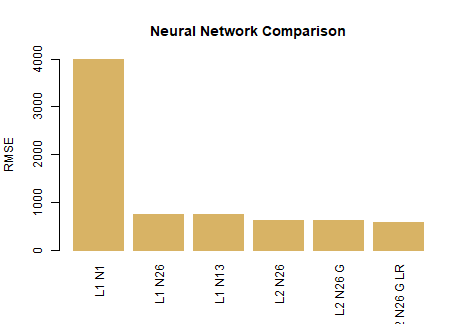
\includegraphics{Diamonds_files/figure-latex/NN Summary-1} \end{center}

\hypertarget{neural-network-graphic-description}{%
\subsubsection{Neural network graphic
description}\label{neural-network-graphic-description}}

\begin{figure}
\centering
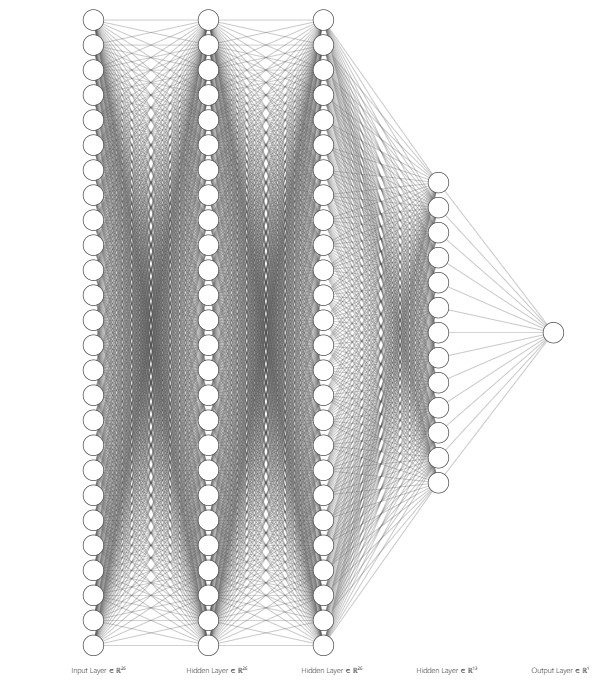
\includegraphics{NN_rep.jpeg}
\caption{Visual description of Neural Network}
\end{figure}

\hypertarget{ensembles}{%
\subsection{Ensembles}\label{ensembles}}

\begin{Shaded}
\begin{Highlighting}[]
\CommentTok{\#create Table with 0 values}
\NormalTok{ensemble\_summ }\OtherTok{\textless{}{-}} \FunctionTok{data.frame}\NormalTok{(}\StringTok{"MLR"} \OtherTok{=} \DecValTok{0}\NormalTok{,}
                             \StringTok{"RegTrees"} \OtherTok{=} \DecValTok{0}\NormalTok{,}
                             \StringTok{"kNN"} \OtherTok{=} \DecValTok{0}\NormalTok{,}
                             \StringTok{"NeuralNets"} \OtherTok{=} \DecValTok{0}\NormalTok{)}
\CommentTok{\#create empty rows}
\NormalTok{ensemble\_summ[}\FunctionTok{length}\NormalTok{(valid.index),] }\OtherTok{\textless{}{-}} \DecValTok{0}

\CommentTok{\#Add values per columns}
\NormalTok{ensemble\_summ[,}\StringTok{"MLR"}\NormalTok{] }\OtherTok{=}\NormalTok{ LM\_Predictions}\SpecialCharTok{$}\NormalTok{LM\_CpAIC\_minus\_corr\_pred}
\NormalTok{ensemble\_summ[,}\StringTok{"RegTrees"}\NormalTok{] }\OtherTok{=}\NormalTok{ pred\_random}
\NormalTok{ensemble\_summ[,}\StringTok{"kNN"}\NormalTok{] }\OtherTok{=}\NormalTok{ opt\_knn\_rescaled\_prices}
\NormalTok{ensemble\_summ[,}\StringTok{"NeuralNets"}\NormalTok{] }\OtherTok{=}\NormalTok{ y\_valid\_pred\_2\_26GLR}

\CommentTok{\#Calculate Average}
\NormalTok{ensemble\_summ}\SpecialCharTok{$}\NormalTok{AveragePred }\OtherTok{\textless{}{-}} \FunctionTok{rowMeans}\NormalTok{(ensemble\_summ[,}\DecValTok{1}\SpecialCharTok{:}\DecValTok{4}\NormalTok{])}
\NormalTok{ensemble\_summ}\SpecialCharTok{$}\NormalTok{RealPrices }\OtherTok{\textless{}{-}}\NormalTok{ real\_prices}

\NormalTok{ens\_error }\OtherTok{=} \FunctionTok{accuracy}\NormalTok{(ensemble\_summ}\SpecialCharTok{$}\NormalTok{AveragePred, ensemble\_summ}\SpecialCharTok{$}\NormalTok{RealPrices)}

\FunctionTok{kable\_styling}\NormalTok{(}\FunctionTok{kable}\NormalTok{(ens\_error)}\SpecialCharTok{\%\textgreater{}\%} \FunctionTok{kable\_classic}\NormalTok{(), }\AttributeTok{full\_width =} \ConstantTok{TRUE}\NormalTok{)}
\end{Highlighting}
\end{Shaded}

\begin{table}
\centering
\begin{tabu} to \linewidth {>{\raggedright}X>{\raggedleft}X>{\raggedleft}X>{\raggedleft}X>{\raggedleft}X>{\raggedleft}X}
\hline
  & ME & RMSE & MAE & MPE & MAPE\\
\hline
Test set & 25.80266 & 582.3353 & 306.1574 & -1.682175 & 8.448477\\
\hline
\end{tabu}
\end{table}

\begin{Shaded}
\begin{Highlighting}[]
\NormalTok{ens\_rmse\_summ \textless{}{-} NN\_res[0,] \#NeuralNet Error}
\NormalTok{ens\_rmse\_summ[1, ] \textless{}{-} round(Acc4, 2)}
\NormalTok{ens\_rmse\_summ[2, ] \textless{}{-} Tree\_res[8,]}
\NormalTok{ens\_rmse\_summ[3, ] \textless{}{-} round(opt\_accuracy, 2)}
\NormalTok{ens\_rmse\_summ[4, ] \textless{}{-} NN\_res[6,]}
\NormalTok{ens\_rmse\_summ[5, ] \textless{}{-} round(ens\_error, 2)}

\NormalTok{row.names(ens\_rmse\_summ) \textless{}{-} c("Multiple Linear Regression",}
\NormalTok{                              "Regression Tree",}
\NormalTok{                              "k{-}Nearest Neighbor",}
\NormalTok{                              "Neural Network",}
\NormalTok{                              "Ensemble")}
\NormalTok{\#display results}
\NormalTok{kable\_styling(kable(ens\_rmse\_summ)\%\textgreater{}\% kable\_classic(), full\_width = FALSE)}
\end{Highlighting}
\end{Shaded}

\hypertarget{model-performance-summary}{%
\section{Model Performance Summary}\label{model-performance-summary}}

\begin{Shaded}
\begin{Highlighting}[]
\NormalTok{predtable\_lr }\OtherTok{\textless{}{-}} \FunctionTok{data.frame}\NormalTok{(}\StringTok{"Real"} \OtherTok{=}\NormalTok{ real\_prices, }
                    \StringTok{"Predicted"} \OtherTok{=}\NormalTok{ ensemble\_summ[, }\DecValTok{1}\NormalTok{],}
                    \StringTok{"Color"} \OtherTok{=}\NormalTok{ diamonds[valid.index, }\DecValTok{3}\NormalTok{],}
                    \StringTok{"Cut"} \OtherTok{=}\NormalTok{ diamonds[valid.index, }\DecValTok{2}\NormalTok{],}
                    \StringTok{"Clarity"} \OtherTok{=}\NormalTok{ diamonds[valid.index, }\DecValTok{4}\NormalTok{])}
\NormalTok{predtable\_rg }\OtherTok{\textless{}{-}} \FunctionTok{data.frame}\NormalTok{(}\StringTok{"Real"} \OtherTok{=}\NormalTok{ real\_prices, }
                    \StringTok{"Predicted"} \OtherTok{=}\NormalTok{ ensemble\_summ[, }\DecValTok{2}\NormalTok{], }
                    \StringTok{"Color"} \OtherTok{=}\NormalTok{ diamonds[valid.index, }\DecValTok{3}\NormalTok{],}
                    \StringTok{"Cut"} \OtherTok{=}\NormalTok{ diamonds[valid.index, }\DecValTok{2}\NormalTok{],}
                    \StringTok{"Clarity"} \OtherTok{=}\NormalTok{ diamonds[valid.index, }\DecValTok{4}\NormalTok{])}
\NormalTok{predtable\_knn }\OtherTok{\textless{}{-}} \FunctionTok{data.frame}\NormalTok{(}\StringTok{"Real"} \OtherTok{=}\NormalTok{ real\_prices, }
                    \StringTok{"Predicted"} \OtherTok{=}\NormalTok{ ensemble\_summ[, }\DecValTok{3}\NormalTok{], }
                    \StringTok{"Color"} \OtherTok{=}\NormalTok{ diamonds[valid.index, }\DecValTok{3}\NormalTok{],}
                    \StringTok{"Cut"} \OtherTok{=}\NormalTok{ diamonds[valid.index, }\DecValTok{2}\NormalTok{],}
                    \StringTok{"Clarity"} \OtherTok{=}\NormalTok{ diamonds[valid.index, }\DecValTok{4}\NormalTok{])}
\NormalTok{predtable\_nn }\OtherTok{\textless{}{-}} \FunctionTok{data.frame}\NormalTok{(}\StringTok{"Real"} \OtherTok{=}\NormalTok{ real\_prices, }
                    \StringTok{"Predicted"} \OtherTok{=}\NormalTok{ ensemble\_summ[, }\DecValTok{4}\NormalTok{], }
                    \StringTok{"Color"} \OtherTok{=}\NormalTok{ diamonds[valid.index, }\DecValTok{3}\NormalTok{],}
                    \StringTok{"Cut"} \OtherTok{=}\NormalTok{ diamonds[valid.index, }\DecValTok{2}\NormalTok{],}
                    \StringTok{"Clarity"} \OtherTok{=}\NormalTok{ diamonds[valid.index, }\DecValTok{4}\NormalTok{])}
\NormalTok{predtable\_ens }\OtherTok{\textless{}{-}} \FunctionTok{data.frame}\NormalTok{(}\StringTok{"Real"} \OtherTok{=}\NormalTok{ real\_prices, }
                    \StringTok{"Predicted"} \OtherTok{=}\NormalTok{ ensemble\_summ[, }\DecValTok{5}\NormalTok{], }
                    \StringTok{"Color"} \OtherTok{=}\NormalTok{ diamonds[valid.index, }\DecValTok{3}\NormalTok{],}
                    \StringTok{"Cut"} \OtherTok{=}\NormalTok{ diamonds[valid.index, }\DecValTok{2}\NormalTok{],}
                    \StringTok{"Clarity"} \OtherTok{=}\NormalTok{ diamonds[valid.index, }\DecValTok{4}\NormalTok{])}


\NormalTok{pred\_plot\_lr }\OtherTok{\textless{}{-}} \FunctionTok{ggplot}\NormalTok{(}\AttributeTok{data =}\NormalTok{ predtable\_lr, }\FunctionTok{aes}\NormalTok{(}\AttributeTok{x=}\NormalTok{ Real, }\AttributeTok{y =}\NormalTok{ Predicted, }\AttributeTok{color =}\NormalTok{ clarity))}\SpecialCharTok{+}
  \FunctionTok{geom\_point}\NormalTok{(}\AttributeTok{show.title =} \ConstantTok{FALSE}\NormalTok{, }\AttributeTok{size =} \FloatTok{0.5}\NormalTok{)}\SpecialCharTok{+}
  \FunctionTok{scale\_color\_brewer}\NormalTok{(}\AttributeTok{type =} \StringTok{\textquotesingle{}div\textquotesingle{}}\NormalTok{, }\AttributeTok{guide =} \FunctionTok{guide\_legend}\NormalTok{(}\AttributeTok{reverse =}\NormalTok{ T, }\AttributeTok{override.aes =} \FunctionTok{list}\NormalTok{(}\AttributeTok{alpha =} \DecValTok{1}\NormalTok{, }\AttributeTok{size =} \FloatTok{0.1}\NormalTok{)))}\SpecialCharTok{+}
  \FunctionTok{labs}\NormalTok{(}\AttributeTok{x=} \StringTok{"Multiple Linear Regression"}\NormalTok{, }\AttributeTok{y =} \StringTok{"Predicted Values"}\NormalTok{)}\SpecialCharTok{+}
  \FunctionTok{theme}\NormalTok{(}\AttributeTok{legend.key.size =} \FunctionTok{unit}\NormalTok{(}\FloatTok{0.5}\NormalTok{, }\StringTok{\textquotesingle{}cm\textquotesingle{}}\NormalTok{))}\SpecialCharTok{+}
  \FunctionTok{theme\_classic}\NormalTok{()}

\NormalTok{pred\_plot\_rg }\OtherTok{\textless{}{-}} \FunctionTok{ggplot}\NormalTok{(}\AttributeTok{data =}\NormalTok{ predtable\_rg, }\FunctionTok{aes}\NormalTok{(}\AttributeTok{x=}\NormalTok{ Real, }\AttributeTok{y =}\NormalTok{ Predicted, }\AttributeTok{color =}\NormalTok{ clarity))}\SpecialCharTok{+}
  \FunctionTok{geom\_point}\NormalTok{(}\AttributeTok{size =} \FloatTok{0.5}\NormalTok{)}\SpecialCharTok{+}
  \FunctionTok{scale\_color\_brewer}\NormalTok{(}\AttributeTok{type =} \StringTok{\textquotesingle{}div\textquotesingle{}}\NormalTok{, }\AttributeTok{guide =} \FunctionTok{guide\_legend}\NormalTok{(}\AttributeTok{reverse =}\NormalTok{ T, }\AttributeTok{override.aes =} \FunctionTok{list}\NormalTok{(}\AttributeTok{alpha =} \DecValTok{1}\NormalTok{, }\AttributeTok{size =} \FloatTok{0.1}\NormalTok{)))}\SpecialCharTok{+}
  \FunctionTok{labs}\NormalTok{(}\AttributeTok{x=} \StringTok{"NN (Regression Trees"}\NormalTok{, }\AttributeTok{y =} \StringTok{""}\NormalTok{)}\SpecialCharTok{+}
  \FunctionTok{theme\_classic}\NormalTok{()}

\NormalTok{pred\_plot\_knn }\OtherTok{\textless{}{-}} \FunctionTok{ggplot}\NormalTok{(}\AttributeTok{data =}\NormalTok{ predtable\_knn, }\FunctionTok{aes}\NormalTok{(}\AttributeTok{x=}\NormalTok{ Real, }\AttributeTok{y =}\NormalTok{ Predicted, }\AttributeTok{color =}\NormalTok{ clarity))}\SpecialCharTok{+}
  \FunctionTok{geom\_point}\NormalTok{(}\AttributeTok{size =} \FloatTok{0.5}\NormalTok{)}\SpecialCharTok{+}
  \FunctionTok{scale\_color\_brewer}\NormalTok{(}\AttributeTok{type =} \StringTok{\textquotesingle{}div\textquotesingle{}}\NormalTok{, }\AttributeTok{guide =} \FunctionTok{guide\_legend}\NormalTok{(}\AttributeTok{reverse =}\NormalTok{ T, }\AttributeTok{override.aes =} \FunctionTok{list}\NormalTok{(}\AttributeTok{alpha =} \DecValTok{1}\NormalTok{, }\AttributeTok{size =} \FloatTok{0.1}\NormalTok{)))}\SpecialCharTok{+}
  \FunctionTok{labs}\NormalTok{(}\AttributeTok{x=} \StringTok{"k Neares Neighbor"}\NormalTok{, }\AttributeTok{y =} \StringTok{""}\NormalTok{)}\SpecialCharTok{+}
  \FunctionTok{theme\_classic}\NormalTok{()}

\NormalTok{pred\_plot\_nn }\OtherTok{\textless{}{-}} \FunctionTok{ggplot}\NormalTok{(}\AttributeTok{data =}\NormalTok{ predtable\_nn, }\FunctionTok{aes}\NormalTok{(}\AttributeTok{x=}\NormalTok{ Real, }\AttributeTok{y =}\NormalTok{ Predicted, }\AttributeTok{color =}\NormalTok{ clarity))}\SpecialCharTok{+}
  \FunctionTok{geom\_point}\NormalTok{(}\AttributeTok{size =} \FloatTok{0.5}\NormalTok{)}\SpecialCharTok{+}
  \FunctionTok{scale\_color\_brewer}\NormalTok{(}\AttributeTok{type =} \StringTok{\textquotesingle{}div\textquotesingle{}}\NormalTok{, }\AttributeTok{guide =} \FunctionTok{guide\_legend}\NormalTok{(}\AttributeTok{reverse =}\NormalTok{ T, }\AttributeTok{override.aes =} \FunctionTok{list}\NormalTok{(}\AttributeTok{alpha =} \DecValTok{1}\NormalTok{, }\AttributeTok{size =} \FloatTok{0.1}\NormalTok{)))}\SpecialCharTok{+}
  \FunctionTok{labs}\NormalTok{(}\AttributeTok{x=} \StringTok{"Neural Networks"}\NormalTok{, }\AttributeTok{y =} \StringTok{""}\NormalTok{)}\SpecialCharTok{+}
  \FunctionTok{theme\_classic}\NormalTok{()}


\NormalTok{pred\_plot\_ens }\OtherTok{\textless{}{-}} \FunctionTok{ggplot}\NormalTok{(}\AttributeTok{data =}\NormalTok{ predtable\_ens, }\FunctionTok{aes}\NormalTok{(}\AttributeTok{x=}\NormalTok{ Real, }\AttributeTok{y =}\NormalTok{ Predicted, }\AttributeTok{color =}\NormalTok{ clarity))}\SpecialCharTok{+}
  \FunctionTok{geom\_point}\NormalTok{(}\AttributeTok{size =} \FloatTok{0.5}\NormalTok{)}\SpecialCharTok{+}
  \FunctionTok{scale\_color\_brewer}\NormalTok{(}\AttributeTok{type =} \StringTok{\textquotesingle{}div\textquotesingle{}}\NormalTok{, }\AttributeTok{guide =} \FunctionTok{guide\_legend}\NormalTok{(}\AttributeTok{reverse =}\NormalTok{ T, }\AttributeTok{override.aes =} \FunctionTok{list}\NormalTok{(}\AttributeTok{alpha =} \DecValTok{1}\NormalTok{, }\AttributeTok{size =} \FloatTok{0.1}\NormalTok{)))}\SpecialCharTok{+}
  \FunctionTok{labs}\NormalTok{(}\AttributeTok{x=} \StringTok{"Ensemble"}\NormalTok{, }\AttributeTok{y =} \StringTok{""}\NormalTok{)}\SpecialCharTok{+}
  \FunctionTok{theme\_classic}\NormalTok{()}

\CommentTok{\#pred\_plot\_full \textless{}{-} grid.arrange(ggplotGrob("Hello"),ggarrange(pred\_plot\_lr, pred\_plot\_rg, pred\_plot\_knn, \#pred\_plot\_nn,pred\_plot\_ens, ncol=2, nrow=3, common.legend = TRUE, legend="right"), nrow = 2)}
\CommentTok{\#pred\_plot\_full}
\end{Highlighting}
\end{Shaded}

\hypertarget{conclusions}{%
\section{Conclusions}\label{conclusions}}

\end{document}
